%----------------------------------------------------------------------------------------
%    PACKAGES AND THEMES
%----------------------------------------------------------------------------------------
\documentclass[aspectratio=169,xcolor=dvipsnames]{beamer}
\makeatletter
\def\input@path{{theme/}}
\makeatother
\usetheme{CleanEasy}
\usepackage[utf8]{inputenc}
\usepackage{lmodern}
\usepackage[T1]{fontenc}
% \usepackage[brazil]{babel}
\usepackage{fix-cm}
\usepackage{amsmath}
\usepackage{mathtools}
\usepackage{listings}
\usepackage{xcolor}
\usepackage{hyperref}
\usepackage{graphicx} % Allows including images
\usepackage{booktabs} % Allows the use of \toprule, \midrule and \bottomrule in tables
\usepackage{tikz}
\usepackage{tcolorbox}
\usetikzlibrary{positioning, shapes, arrows, calc, decorations.pathreplacing, arrows.meta, backgrounds, patterns, overlay-beamer-styles}
\usepackage{etoolbox}
\usepackage{animate}
\definecolor{uvablue}{RGB}{35,45,75}
\definecolor{uvaorange}{RGB}{229,114,0}
\definecolor{UniBlue}{RGB}{83,121,170}
\definecolor{forestgreen}{RGB}{0,128,0}
\definecolor{bronze}{rgb}{0.8, 0.5, 0.2}
\definecolor{purple}{RGB}{128,0,128}
\definecolor{maroon}{RGB}{184,15,10}
\definecolor{grey}{RGB}{128,128,128}
\definecolor{bondiblue}{rgb}{0.0, 0.58, 0.71}
\definecolor{gold}{RGB}{160,116,10}
\definecolor{peacockblue}{RGB}{0,164,180}
\definecolor{pastelblue}{RGB}{174, 198,207}
\definecolor{pastelgreen}{RGB}{170, 208, 179}
\definecolor{darkblue}{RGB}{0,90, 142}
\definecolor{olivegreen}{RGB}{0, 73, 63}
\usepackage{ragged2e}
%----------------------------------------------------------------------------------------
%    LAYOUT CONFIGURATION
%----------------------------------------------------------------------------------------
\input{configs/configs}
%----------------------------------------------------------------------------------------
%    TITLE PAGE
%----------------------------------------------------------------------------------------


%---------------------------------------------


\title[Background Estimation Procedure]{Background Estimation Procedure}

\author[S. Campbell]{Samuel Campbell\inst{1}}

\institute[UA]{\inst{1}%
  Graduate Student\\
  University of Alabama
}


\vspace{-2cm}\date{\today}
% Define positions for logos on title page
\titlegraphic{
  \begin{tikzpicture}[remember picture, overlay]
    % 
    \node[anchor=south west, xshift=0.5cm, yshift=0cm] at (current page.south west) {
      
\includegraphics[height=1.3cm]{logos/cms.png}
    };
  
    % 
    \node[anchor=north east, xshift=-0.8cm, yshift=-0.3cm] at (current page.north east) {
      
\includegraphics[height=1.1cm]{logos/University-of-Alabama-Logo.png}
    };
  \end{tikzpicture}
}


%----------------------------------------------------------------------------------------


\begin{document}

\begin{frame}[plain]
  \titlepage
\end{frame}

\begin{frame}[plain]{Contents}
  \tableofcontents
\end{frame}

\section{Introduction}
\begin{frame}{Introduction}
    \begin{itemize}
        \item I made 2D Distributions of $\mu$-LJ isolation vs Pixel Hits
        \item The only event cut required is that $\Delta \phi \geq 2$
        \item I made these plots for the following categories:
        \begin{itemize}
            \item Total Background
            \item QCD Only
            \item TTJets Only
            \item Signal Only (Average $L_{xy} = 30.0$ cm)
        \end{itemize}
    \end{itemize}
\end{frame}

\begin{frame}{Total Background}
    \centering
    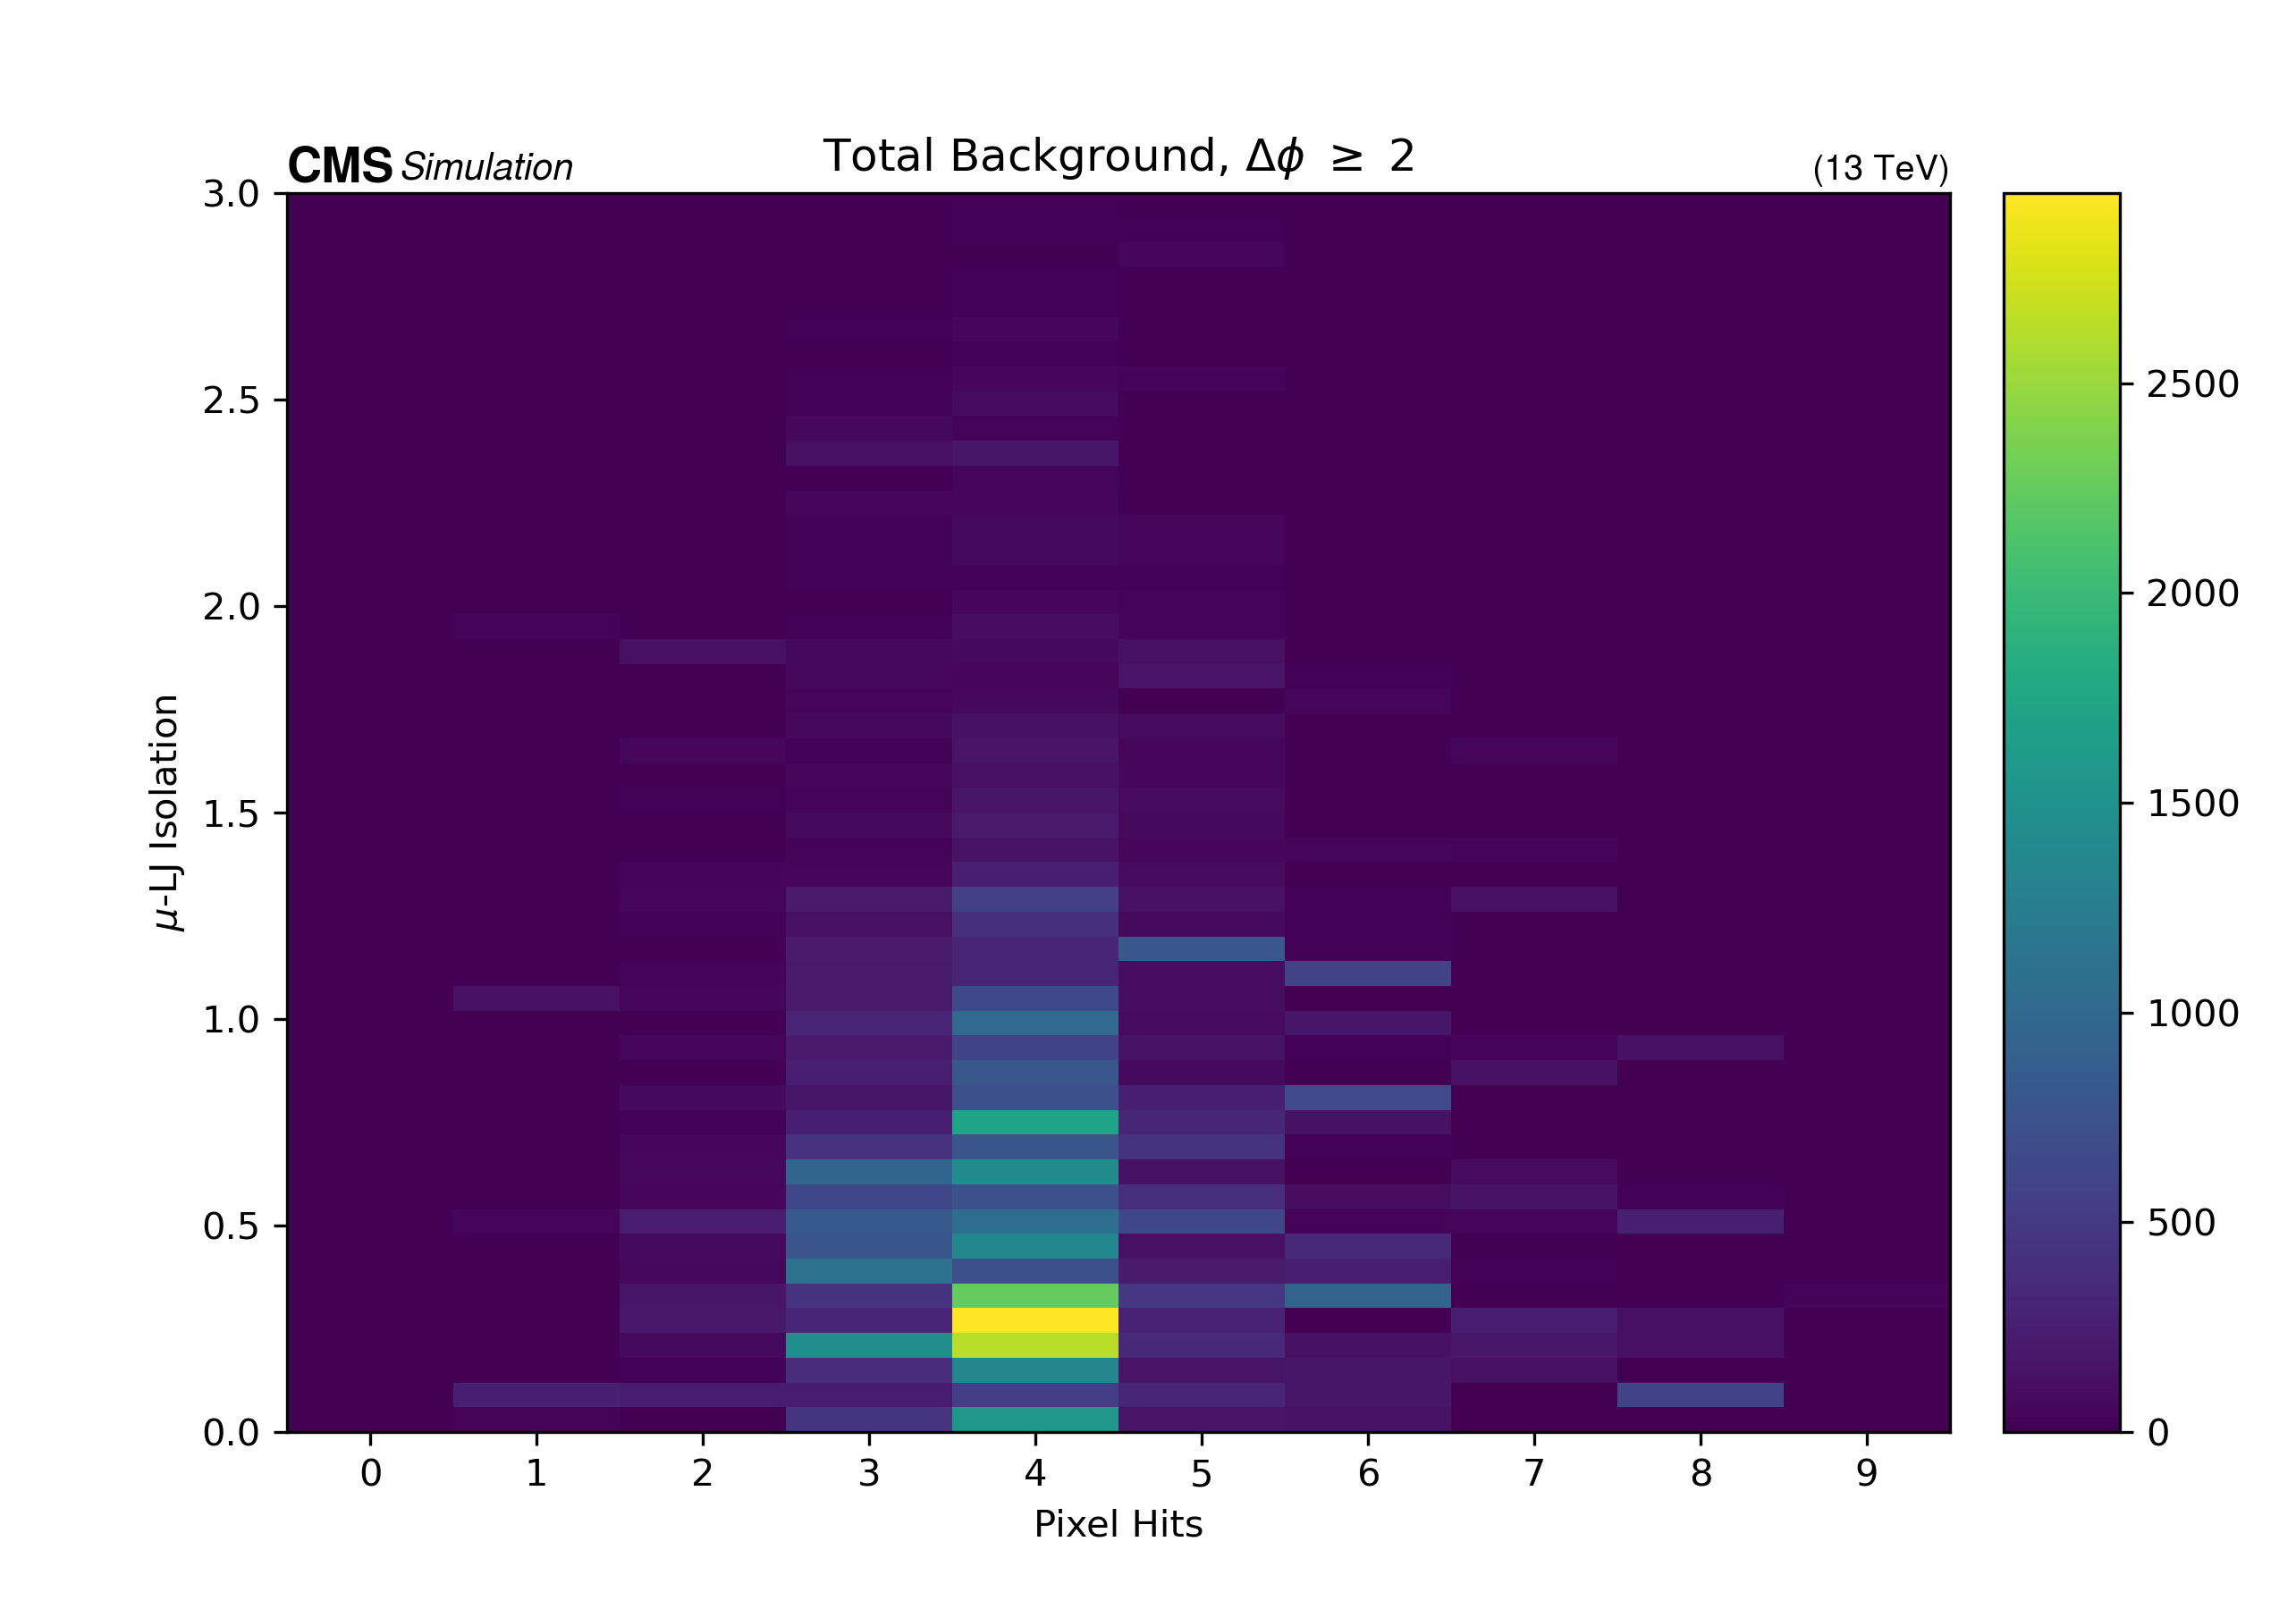
\includegraphics[width=0.7\linewidth]{figures/2D_mJIso_vs_pixelHits_total_background.png}
\end{frame}

\begin{frame}{QCD Only}
    \centering
    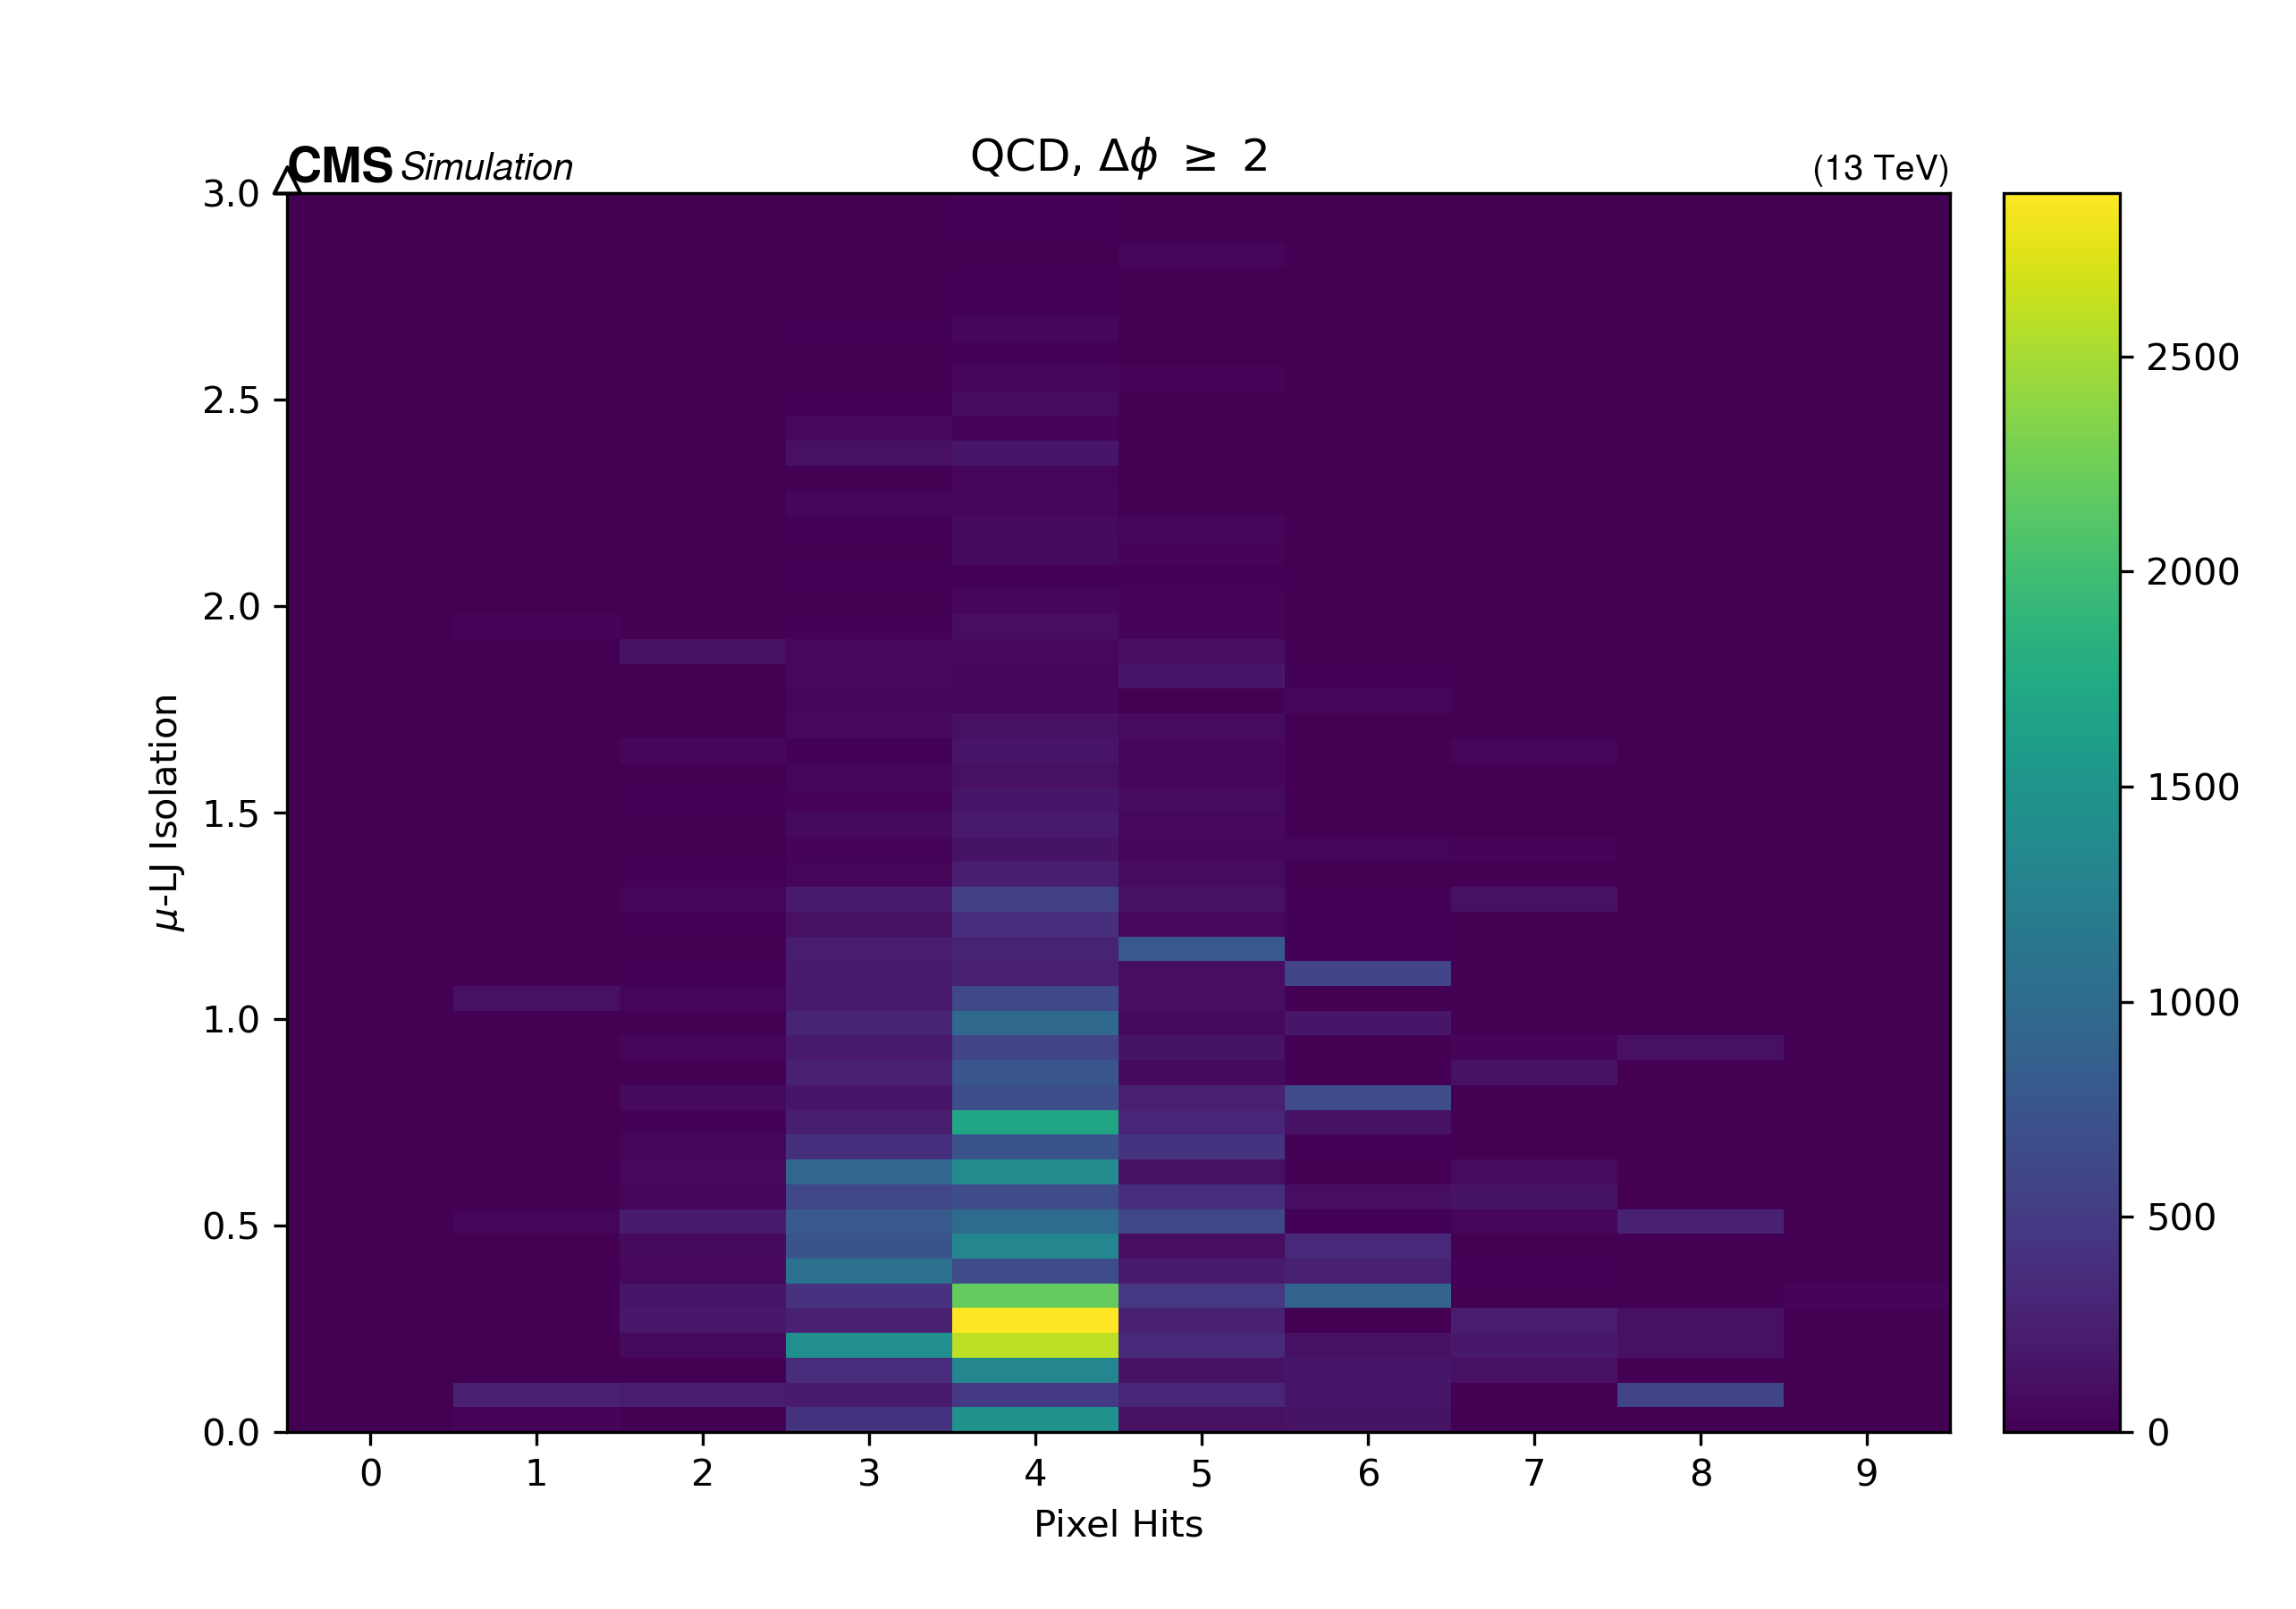
\includegraphics[width=0.7\linewidth]{figures/2D_mJIso_vs_pixelHits_qcd.png}
\end{frame}

\begin{frame}{TTJets Only}
    \centering
    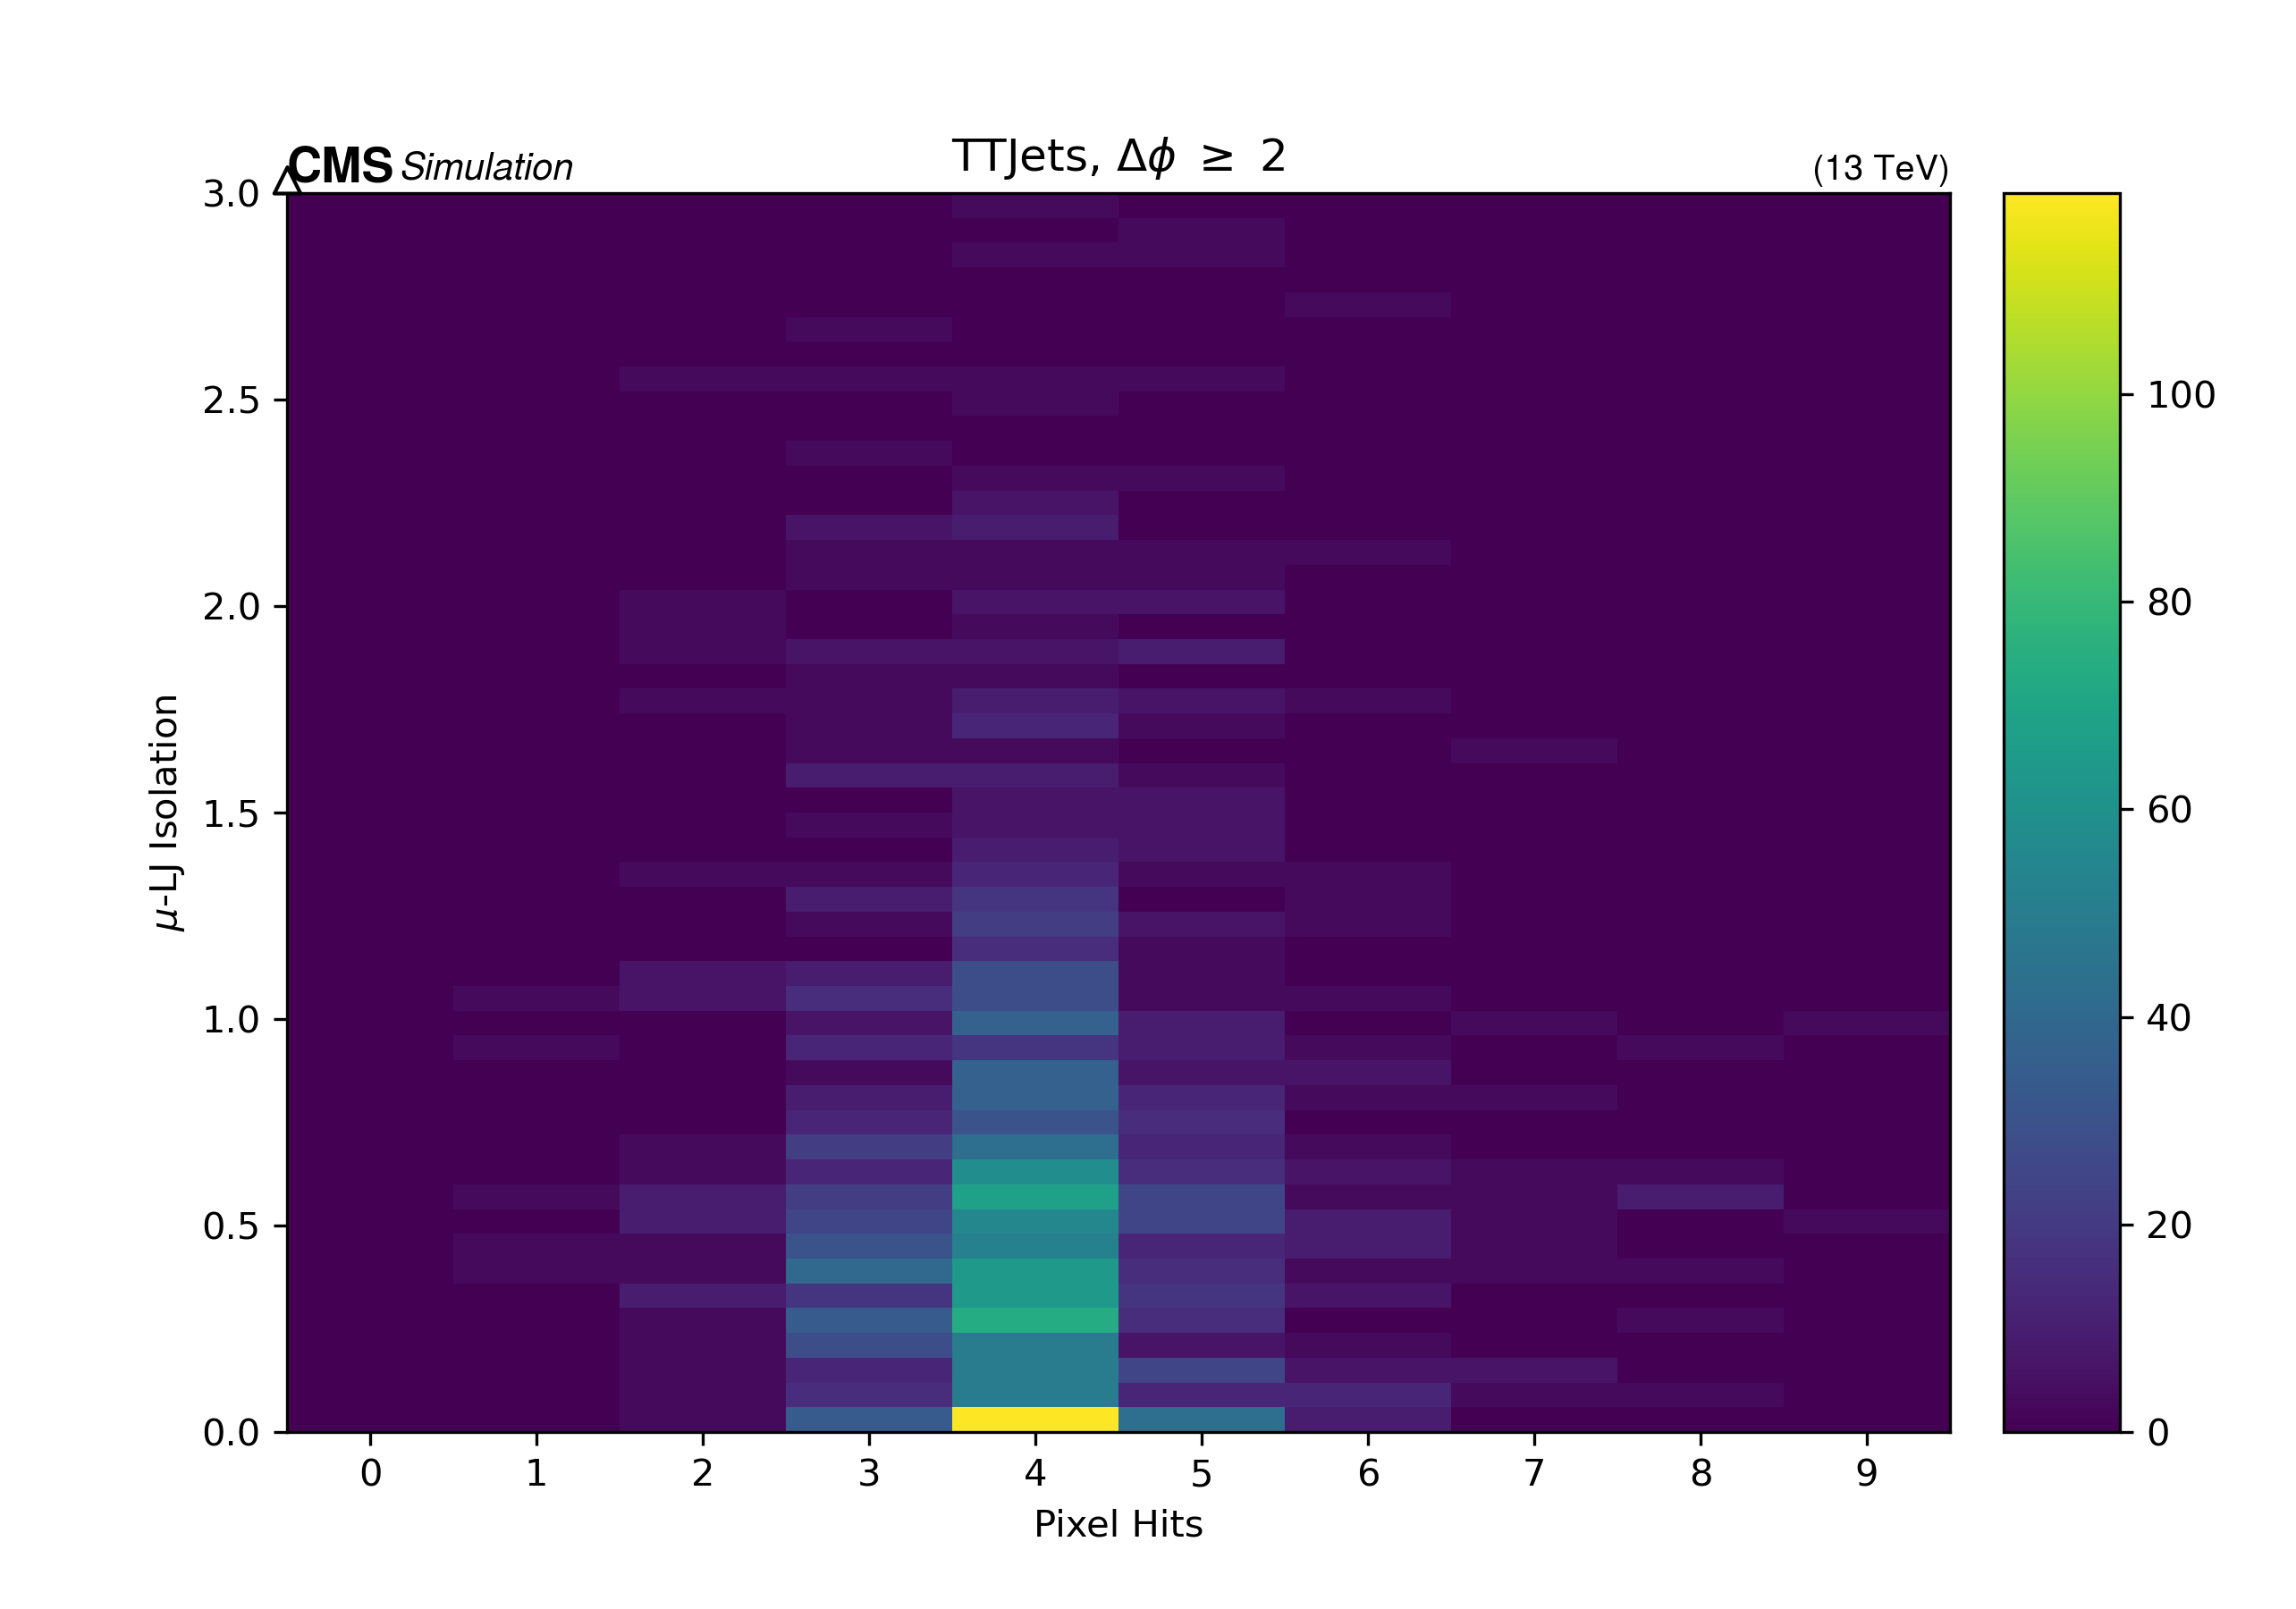
\includegraphics[width=0.7\linewidth]{figures/2D_mJIso_vs_pixelHits_ttjets.png}
\end{frame}

\begin{frame}{Backgrounds Comparison}
    \begin{columns}
        \begin{column}{0.333\textwidth}
            \centering
            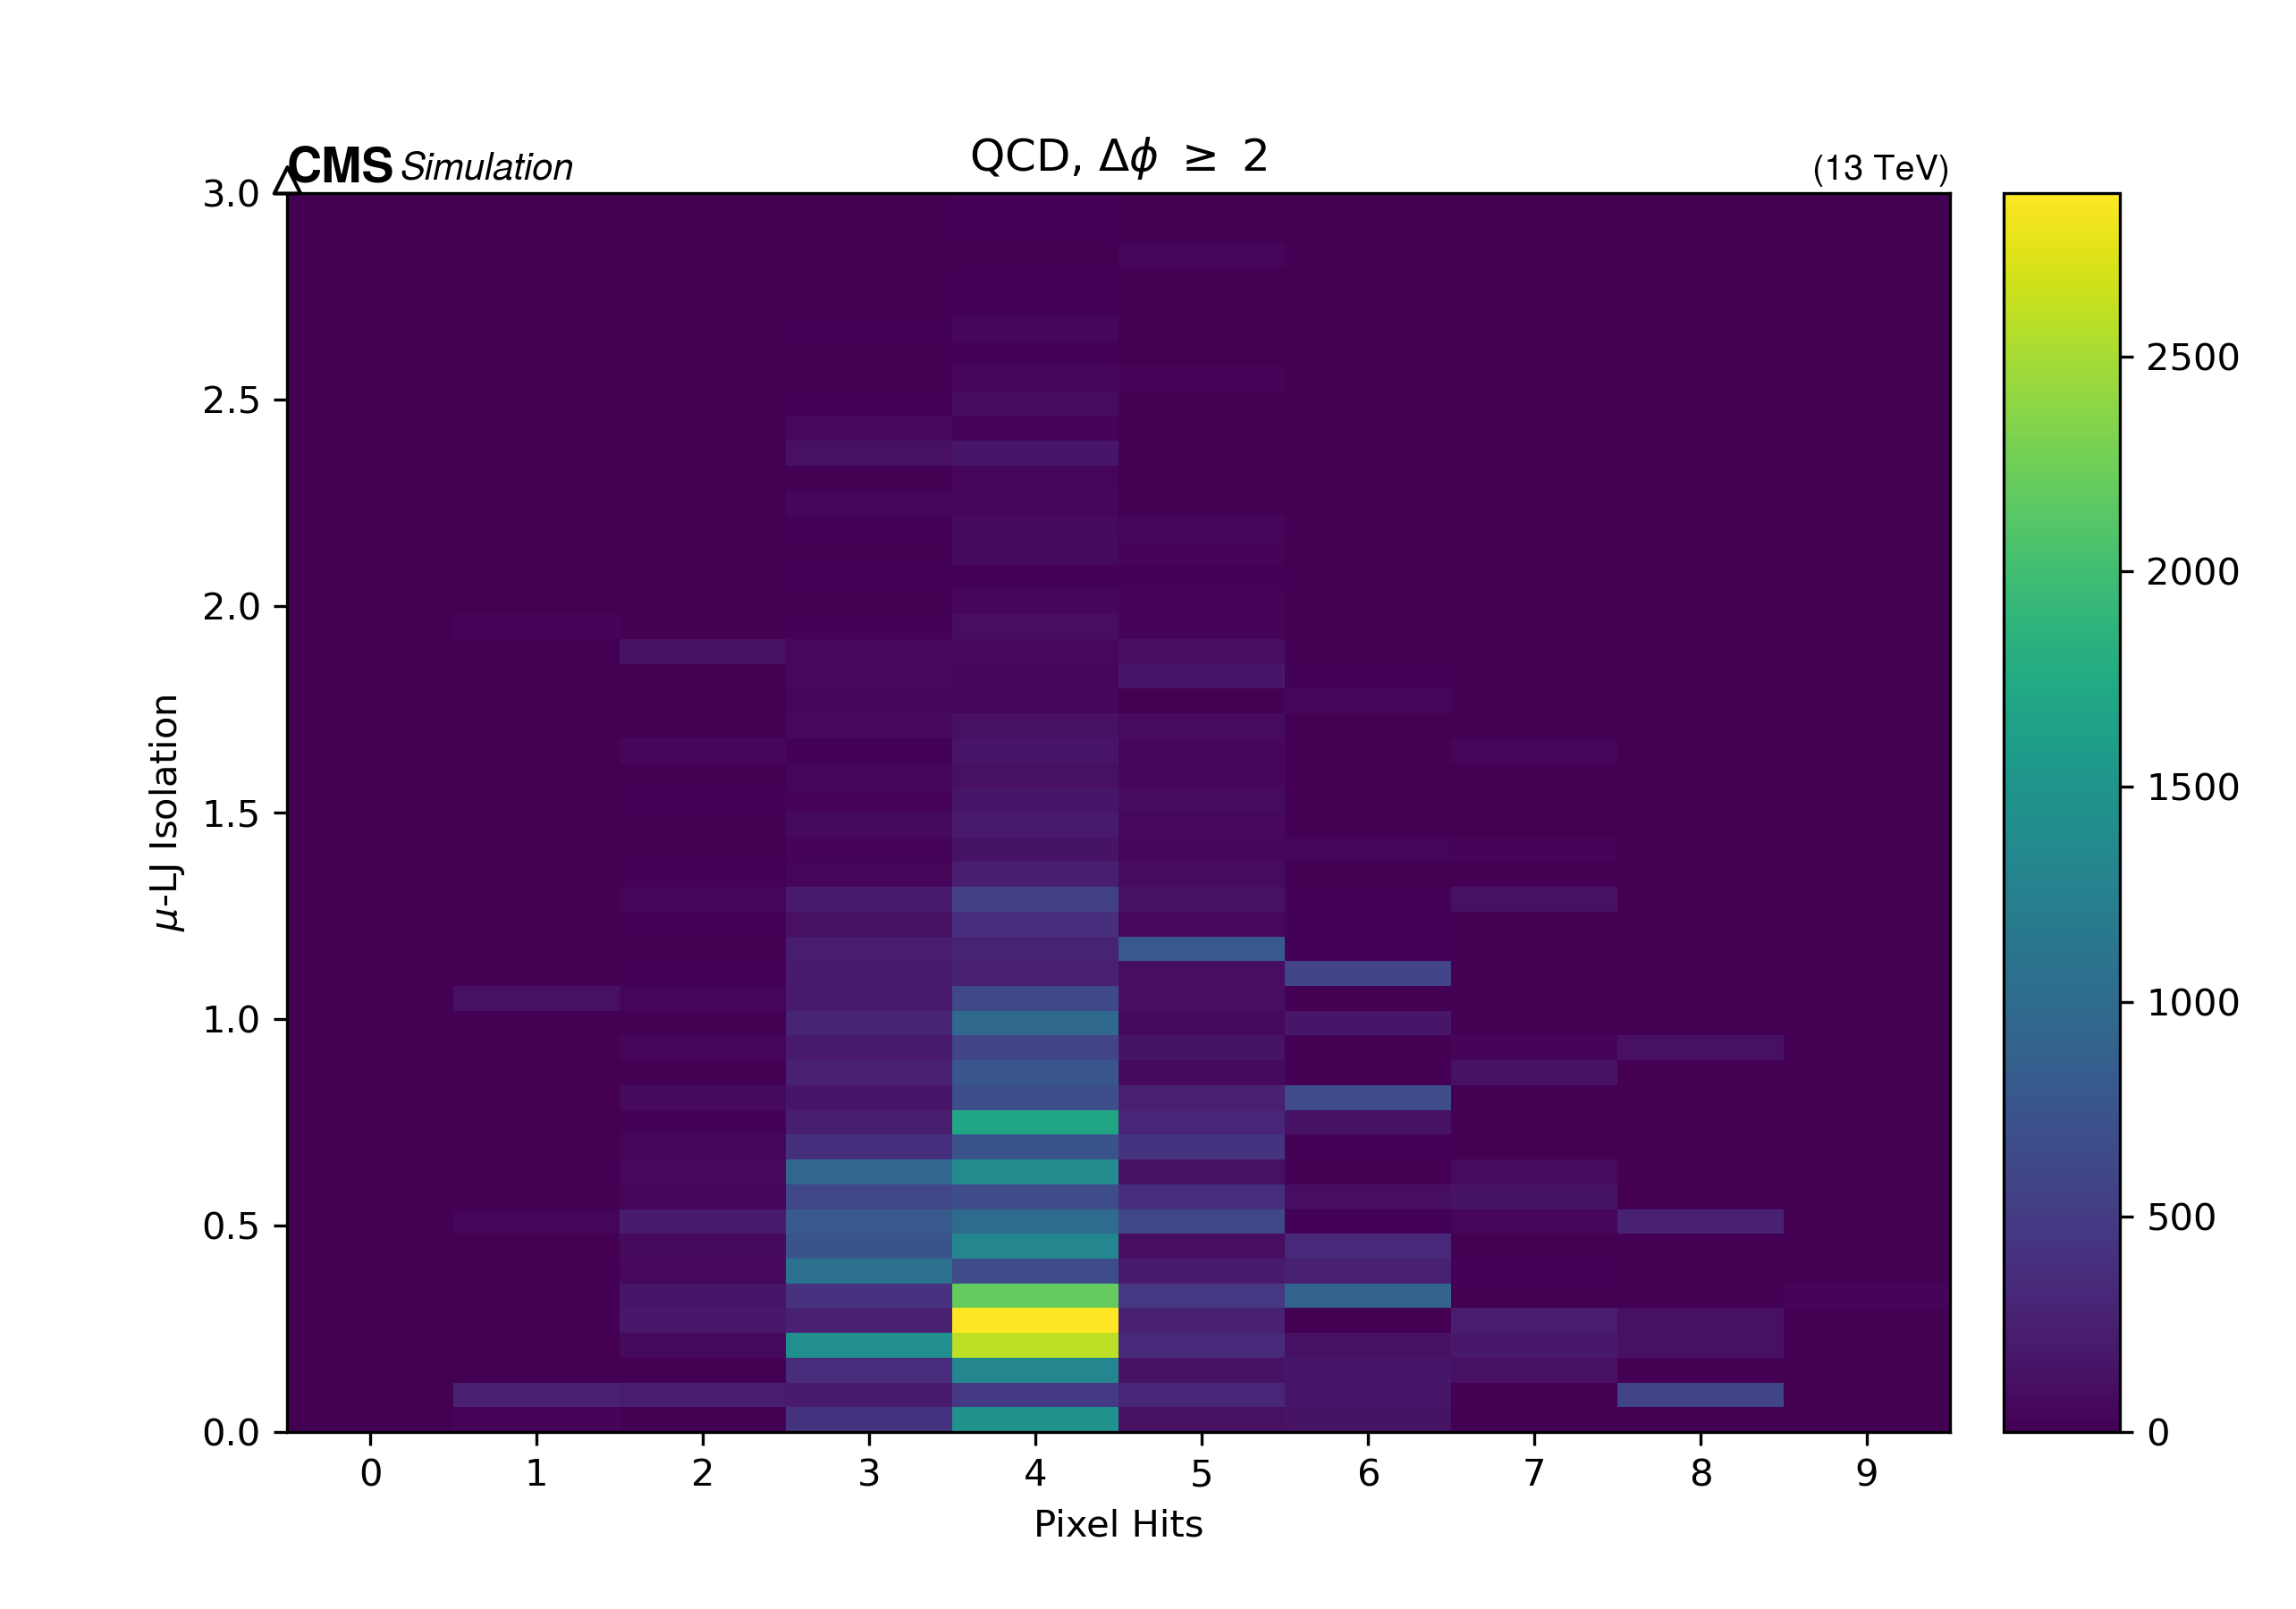
\includegraphics[width=\linewidth]{figures/2D_mJIso_vs_pixelHits_qcd.png}
        \end{column}
        \begin{column}{0.333\textwidth}
            \centering 
            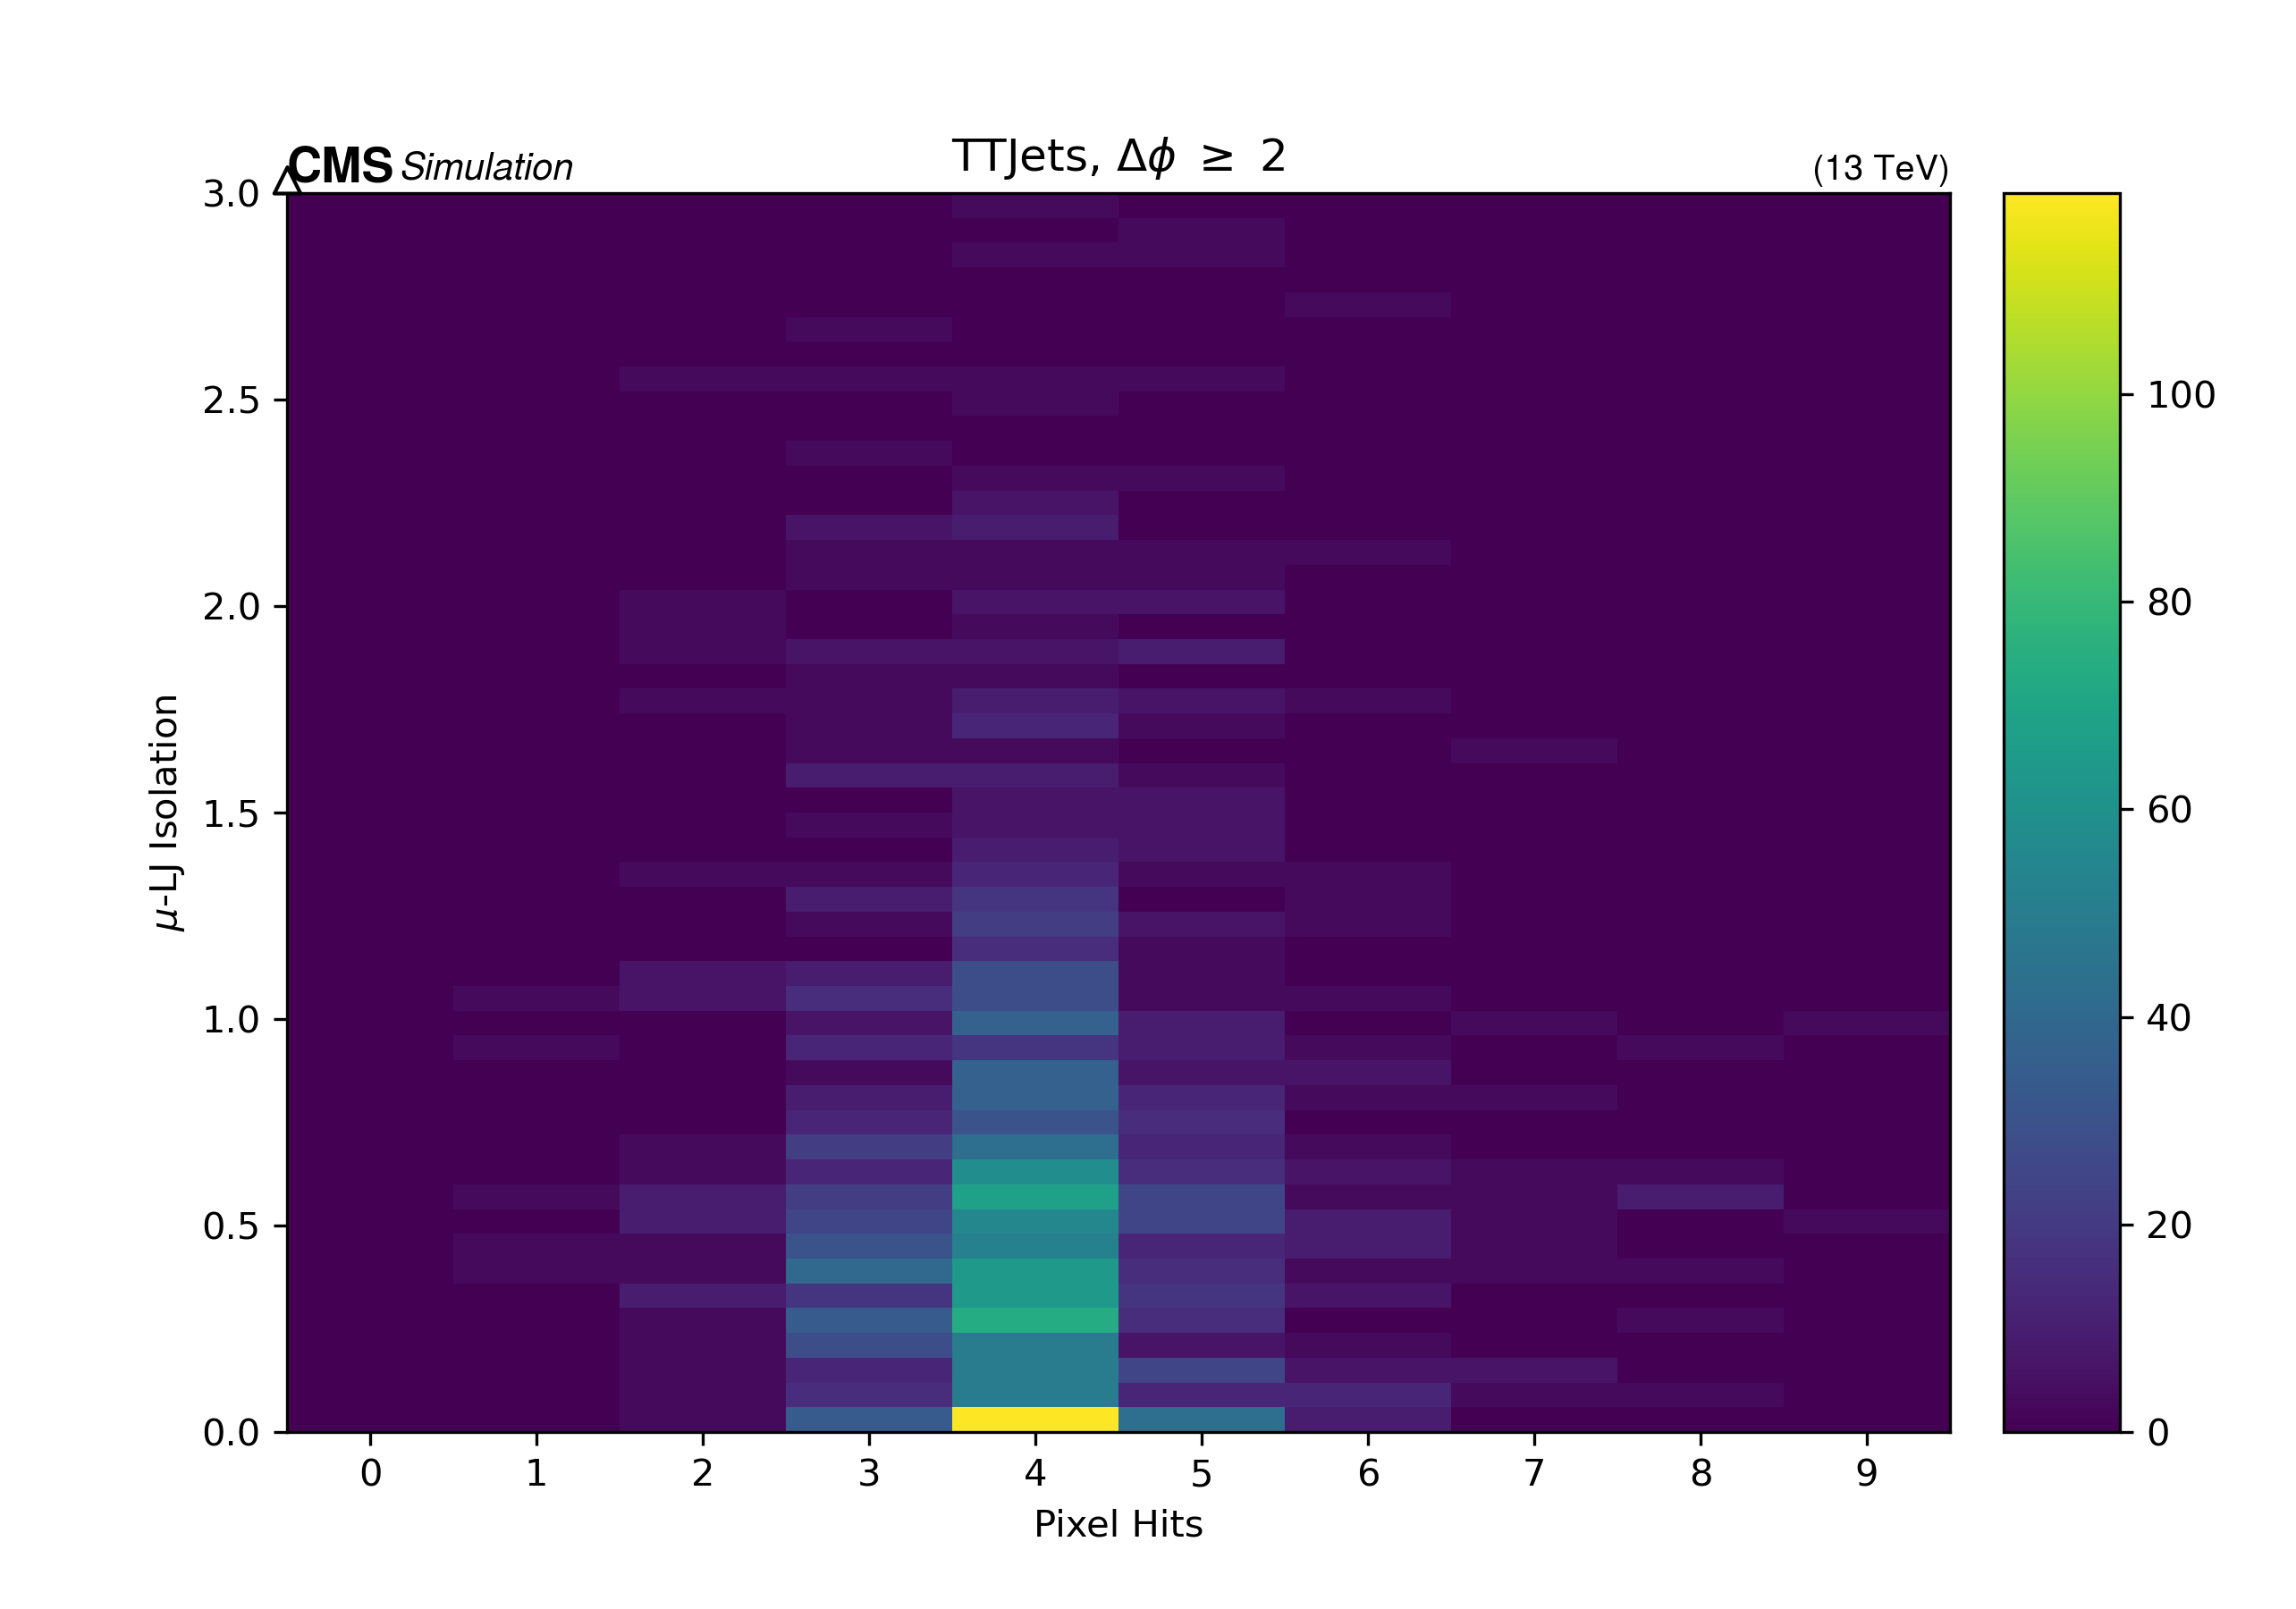
\includegraphics[width=\linewidth]{figures/2D_mJIso_vs_pixelHits_ttjets.png}
        \end{column}
        \begin{column}{0.333\textwidth}
            \centering 
            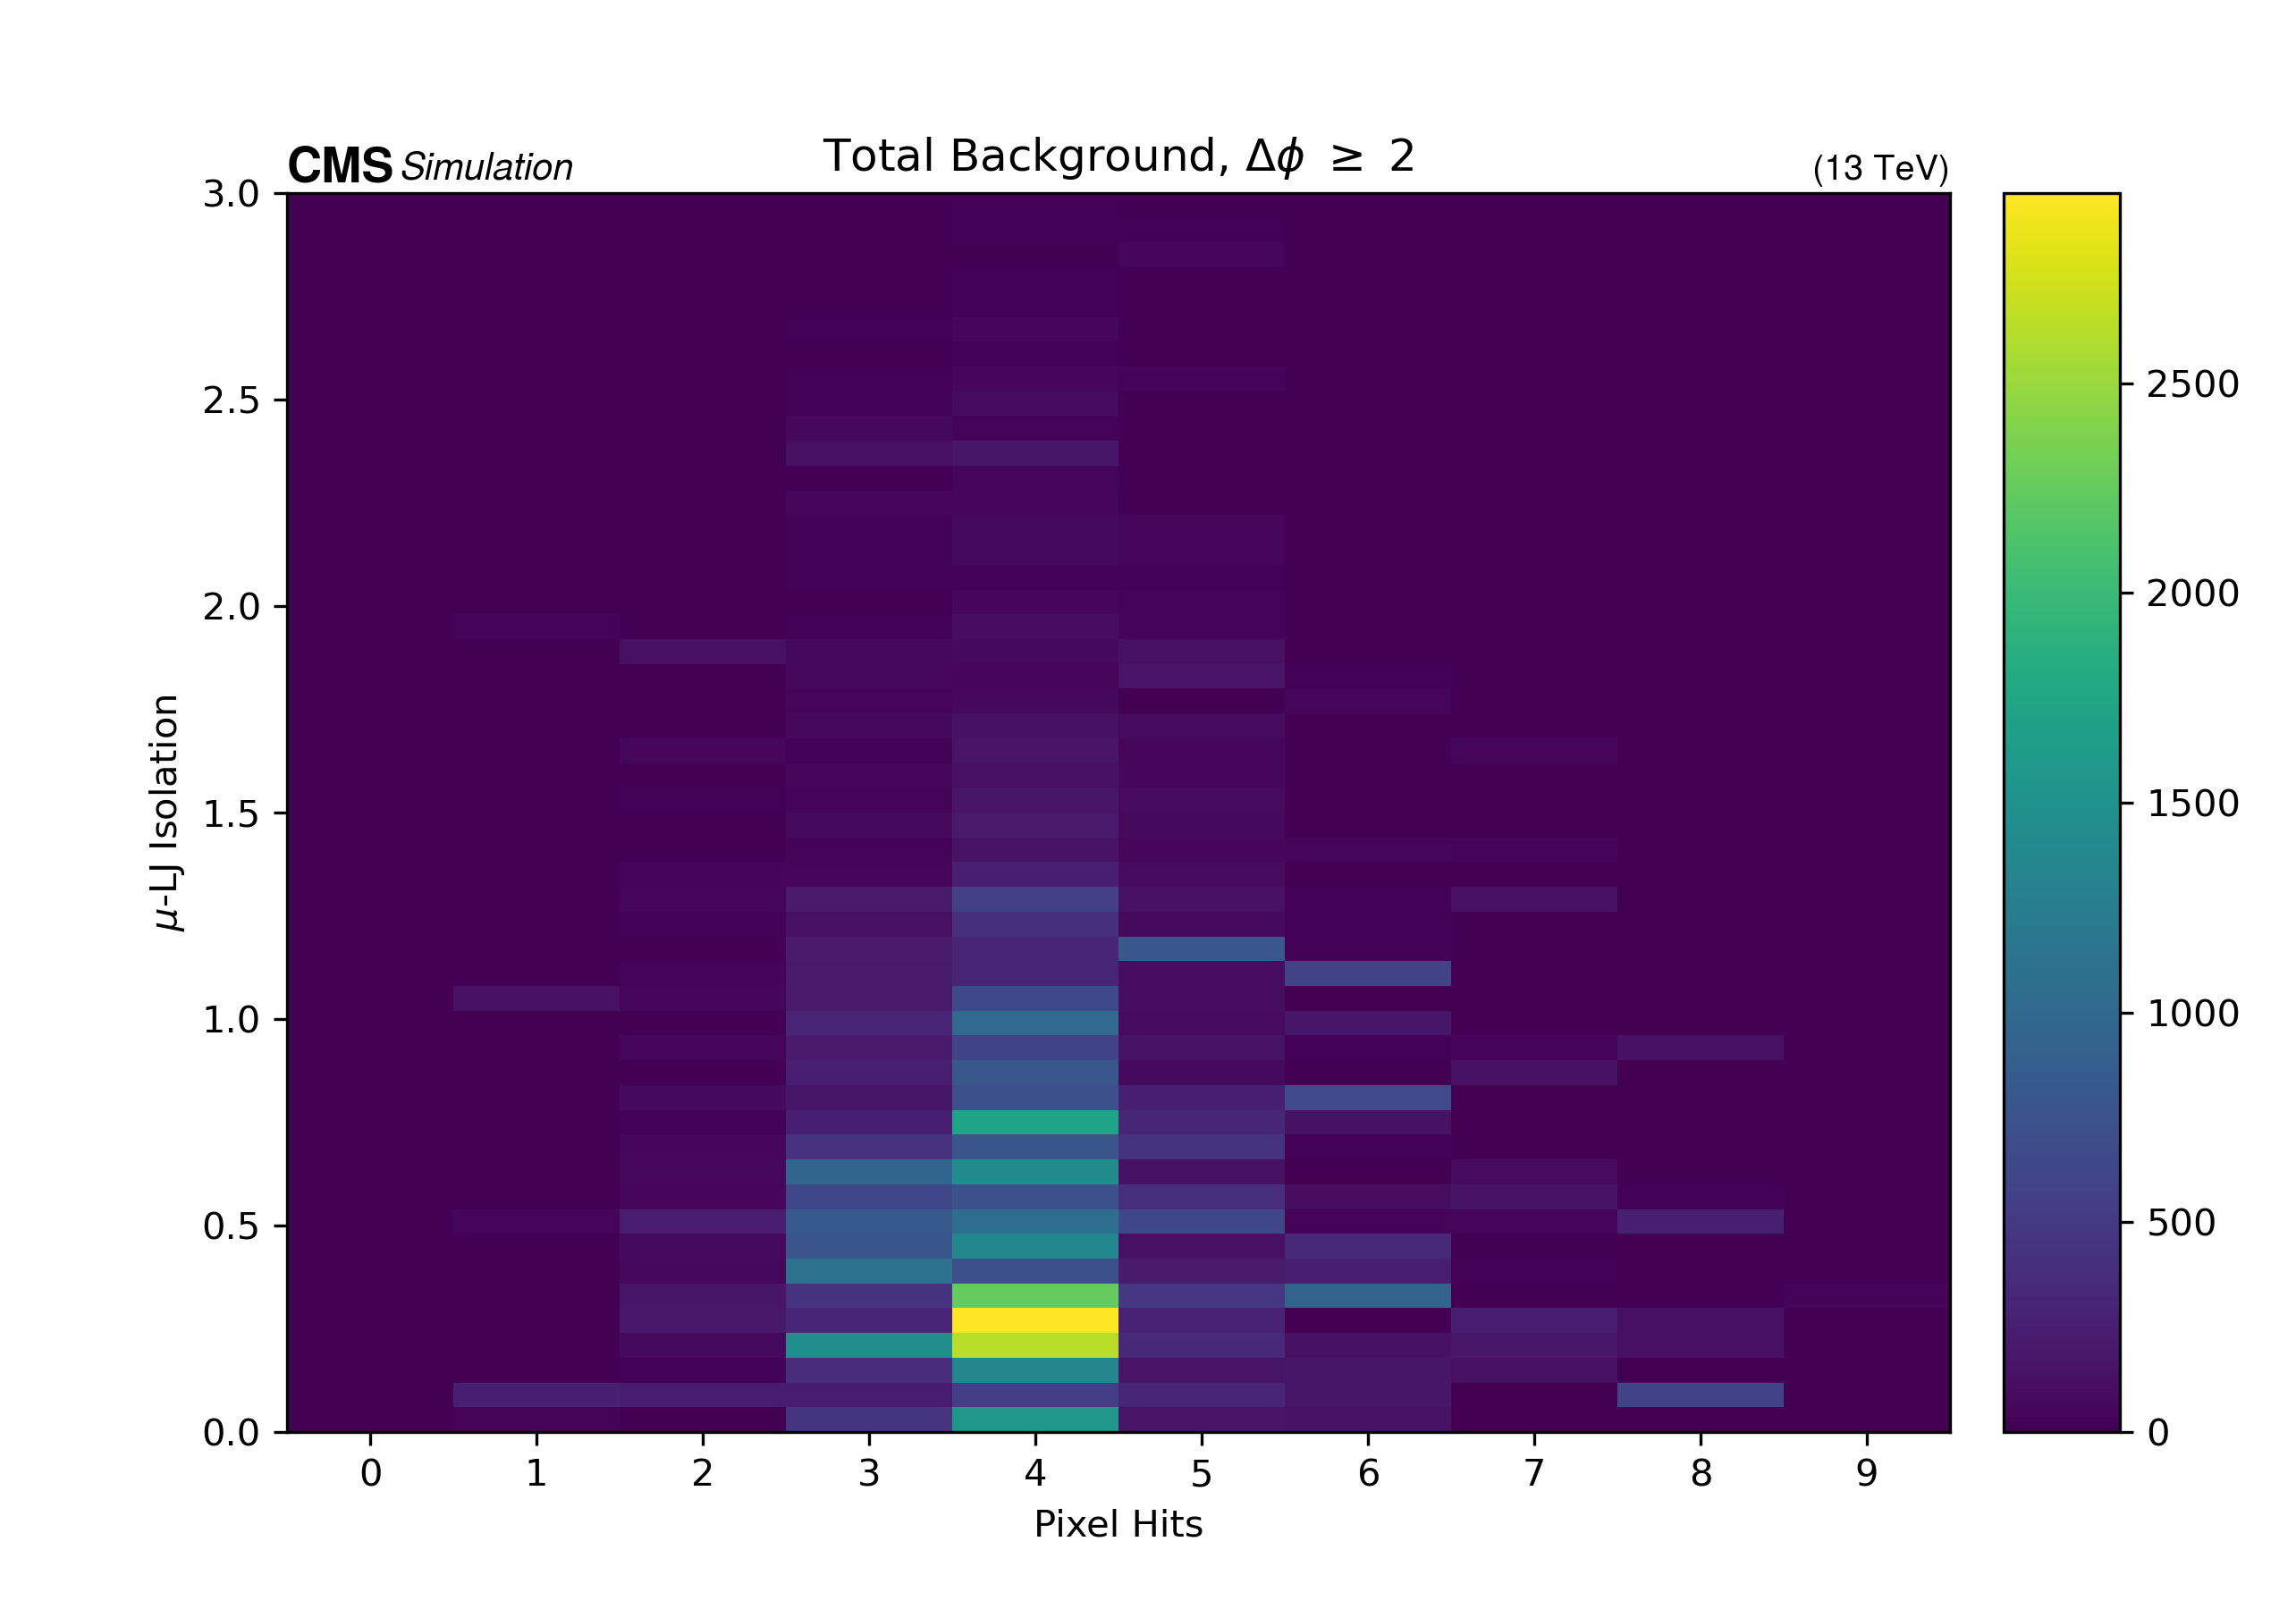
\includegraphics[width=\linewidth]{figures/2D_mJIso_vs_pixelHits_total_background.png}
        \end{column}
    \end{columns}
\end{frame}

\begin{frame}{200 GeV}
	\centering
	\begin{columns}
		\begin{column}{0.333\textwidth}
			\centering
			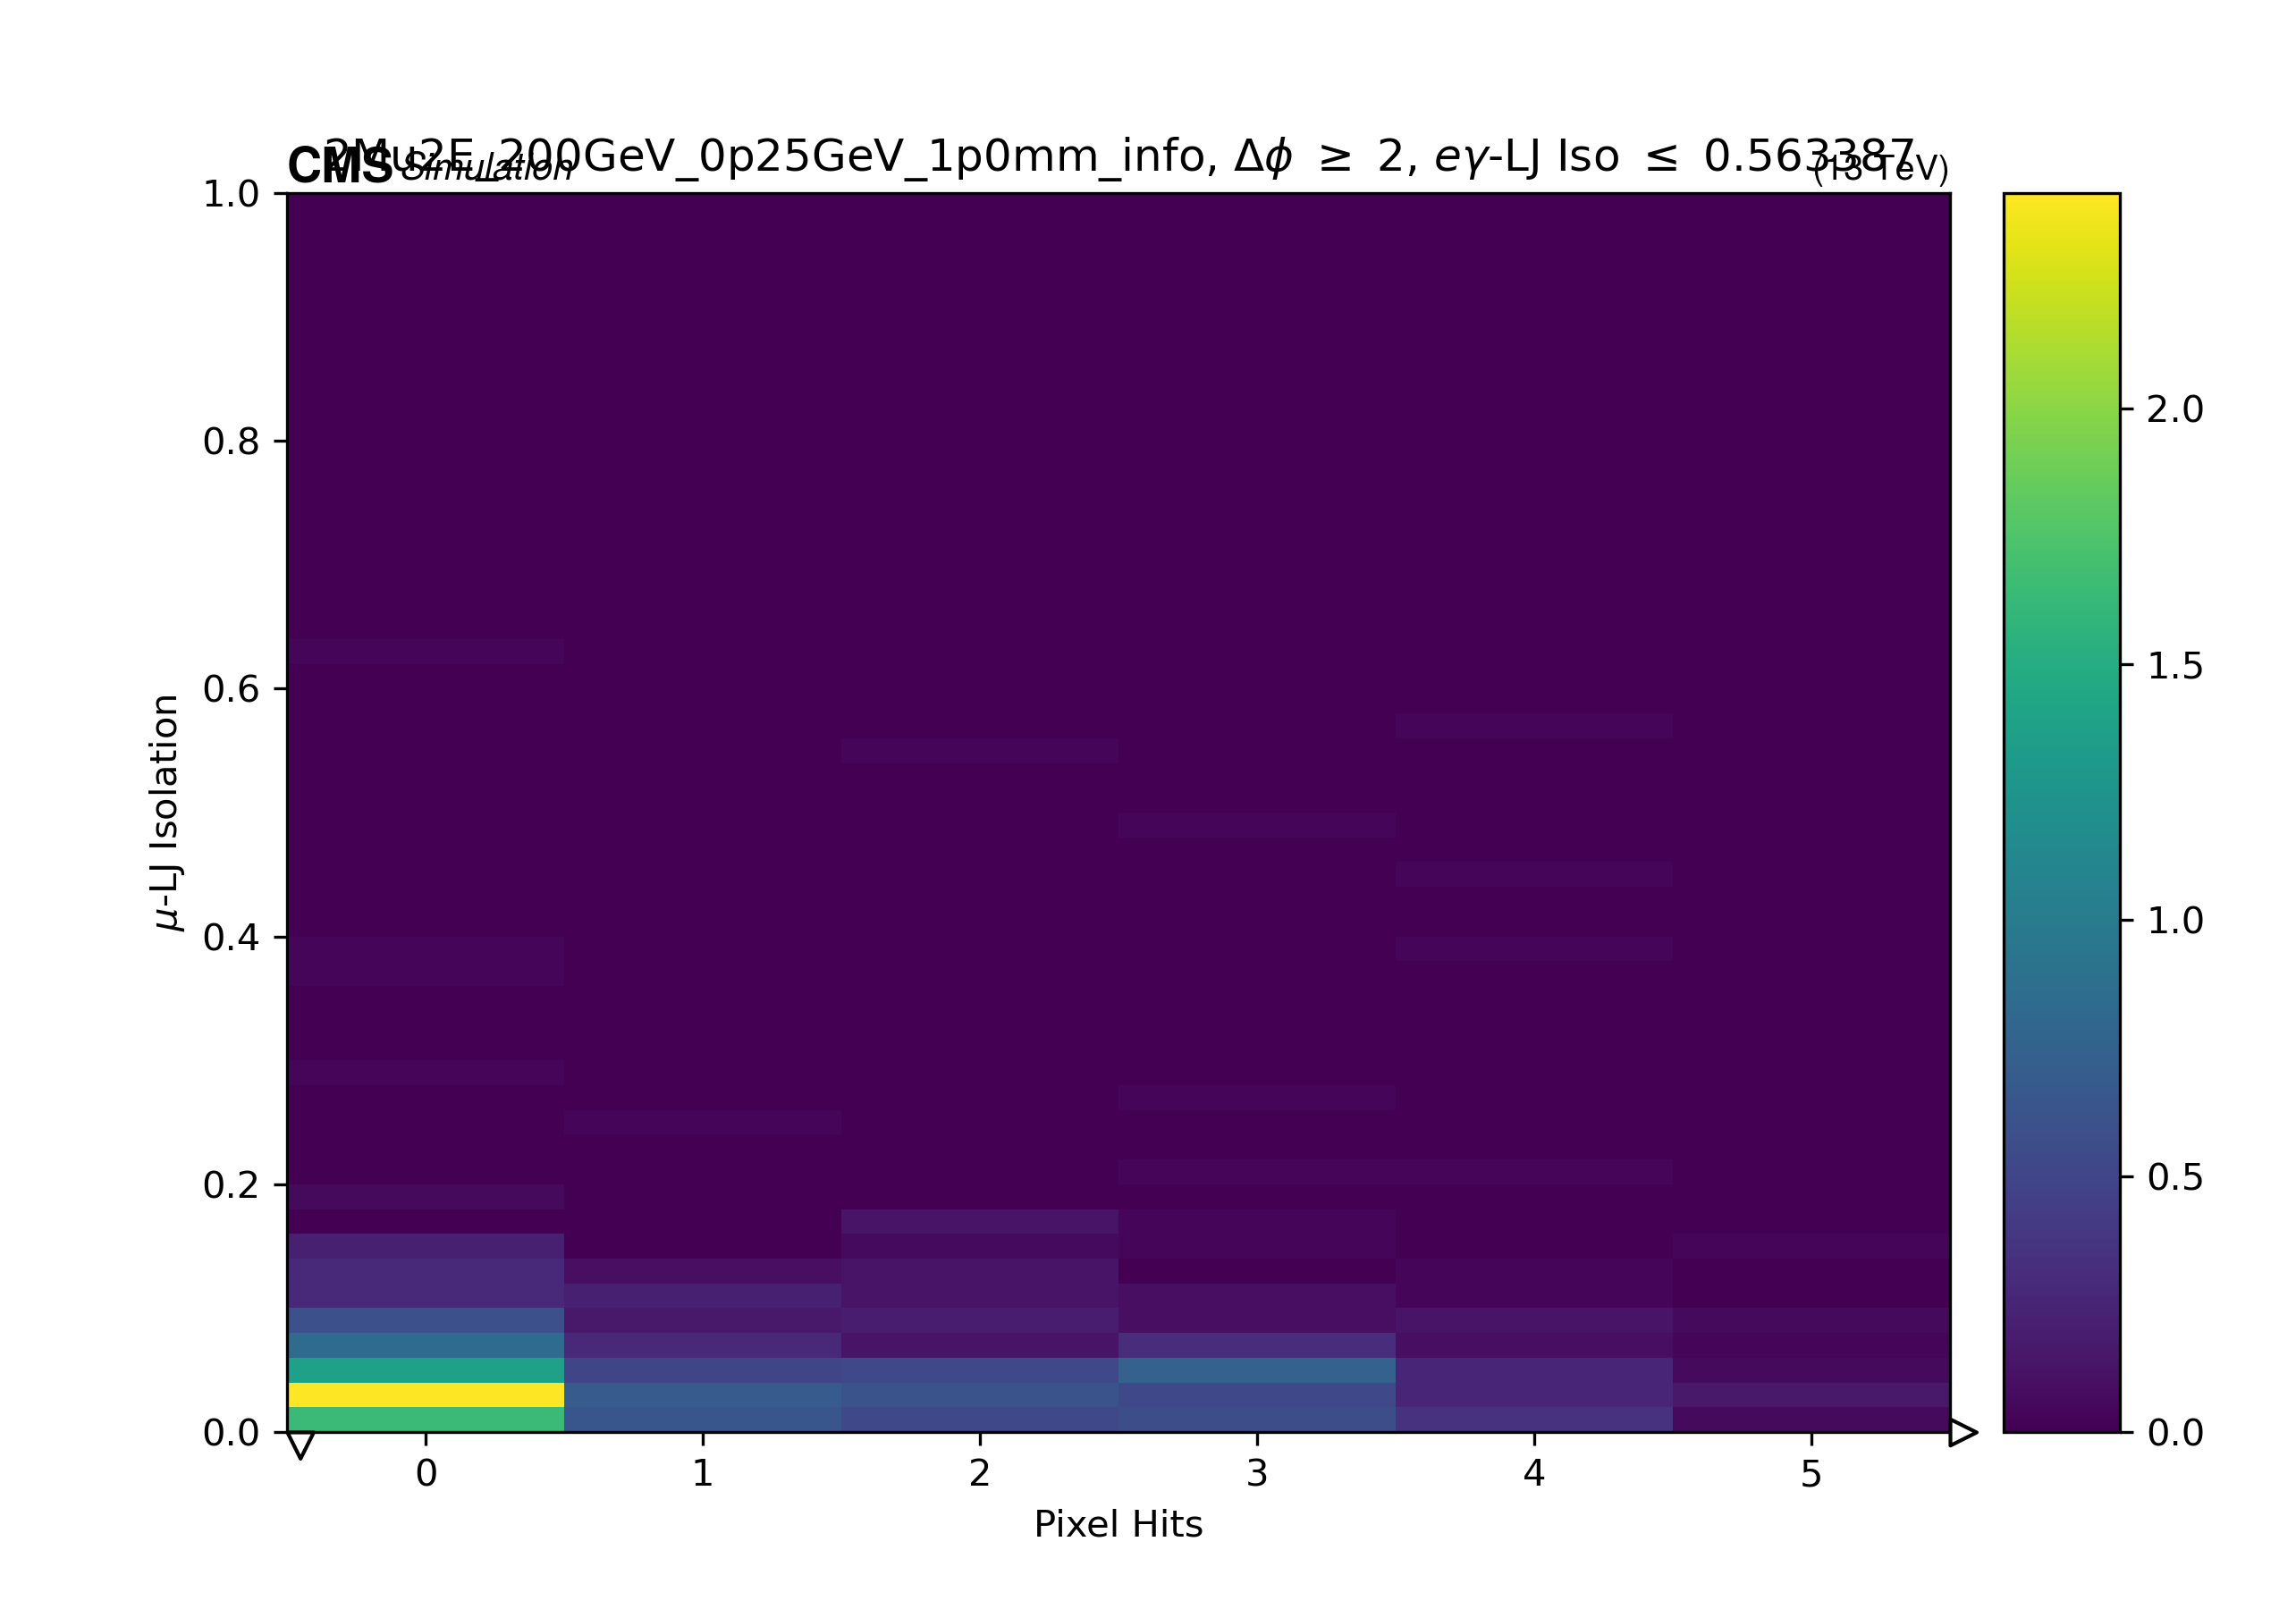
\includegraphics[width=\linewidth]{figures/2D_mJIso_vs_pixelHits_2Mu2E_200GeV_0p25GeV_1p0mm_info.png}
		\end{column}
		\begin{column}{0.333\textwidth}
			\centering
			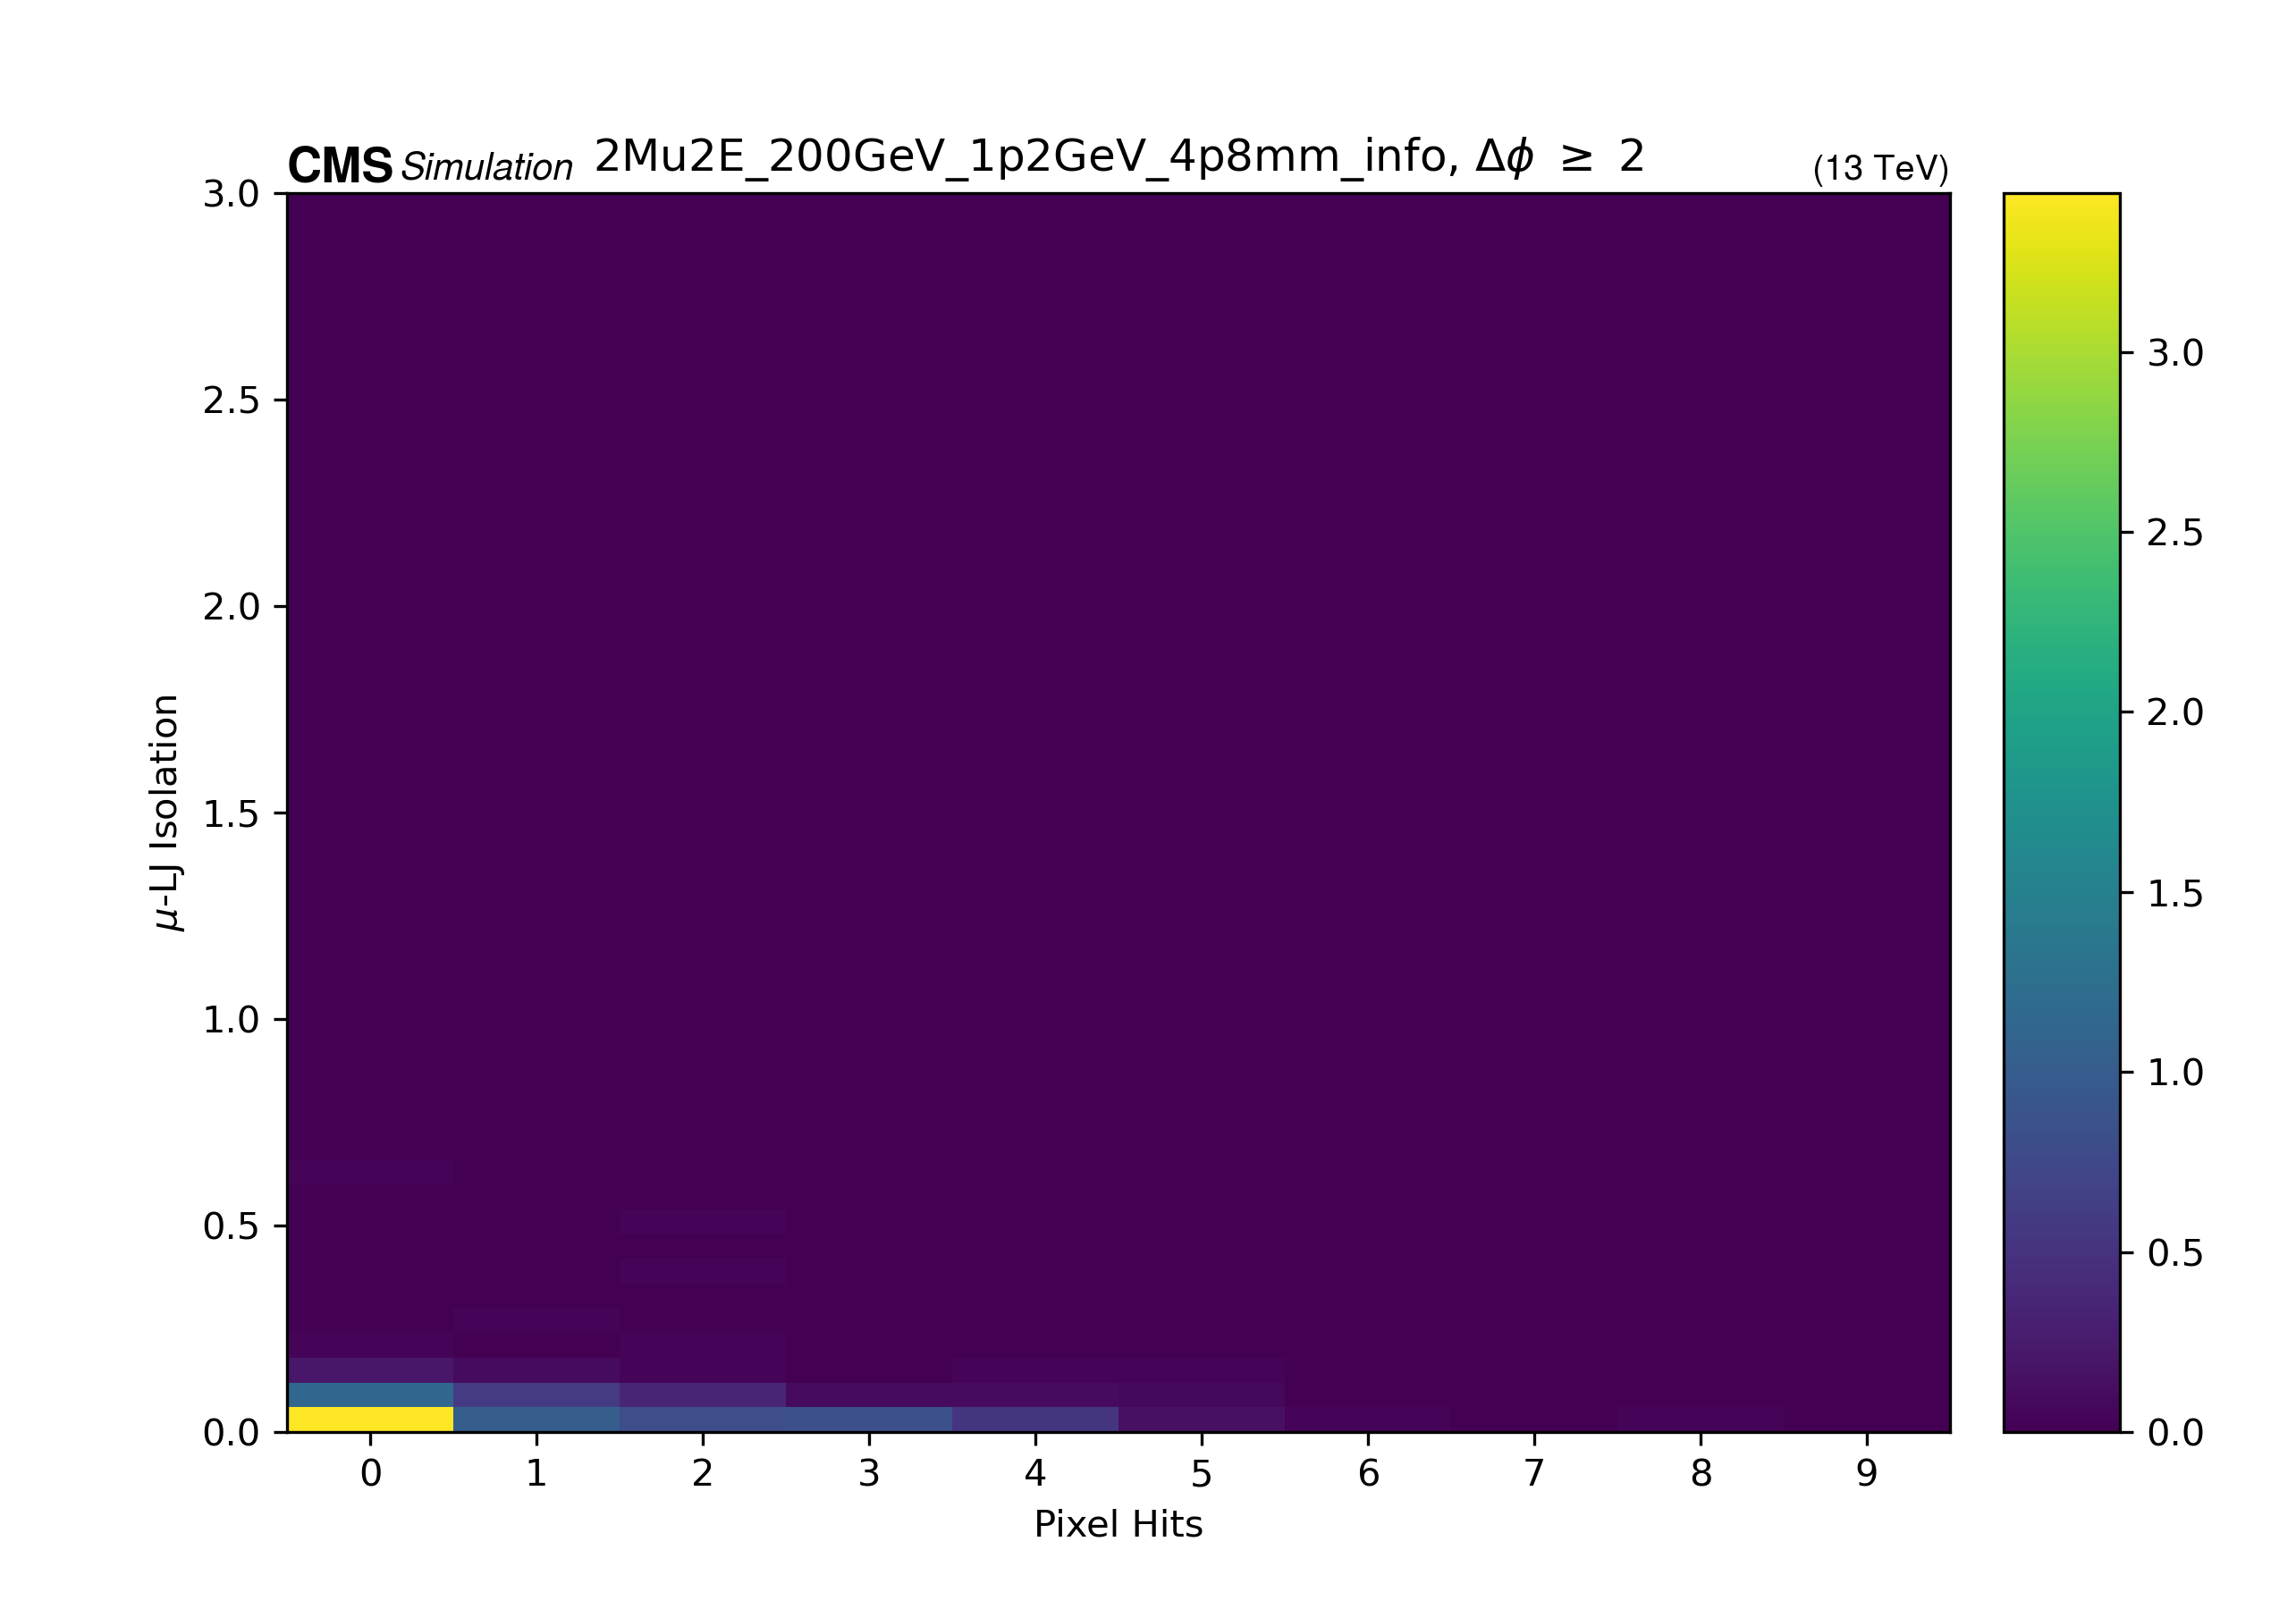
\includegraphics[width=\linewidth]{figures/2D_mJIso_vs_pixelHits_2Mu2E_200GeV_1p2GeV_4p8mm_info.png}
		\end{column}
		\begin{column}{0.333\textwidth}
			\centering
			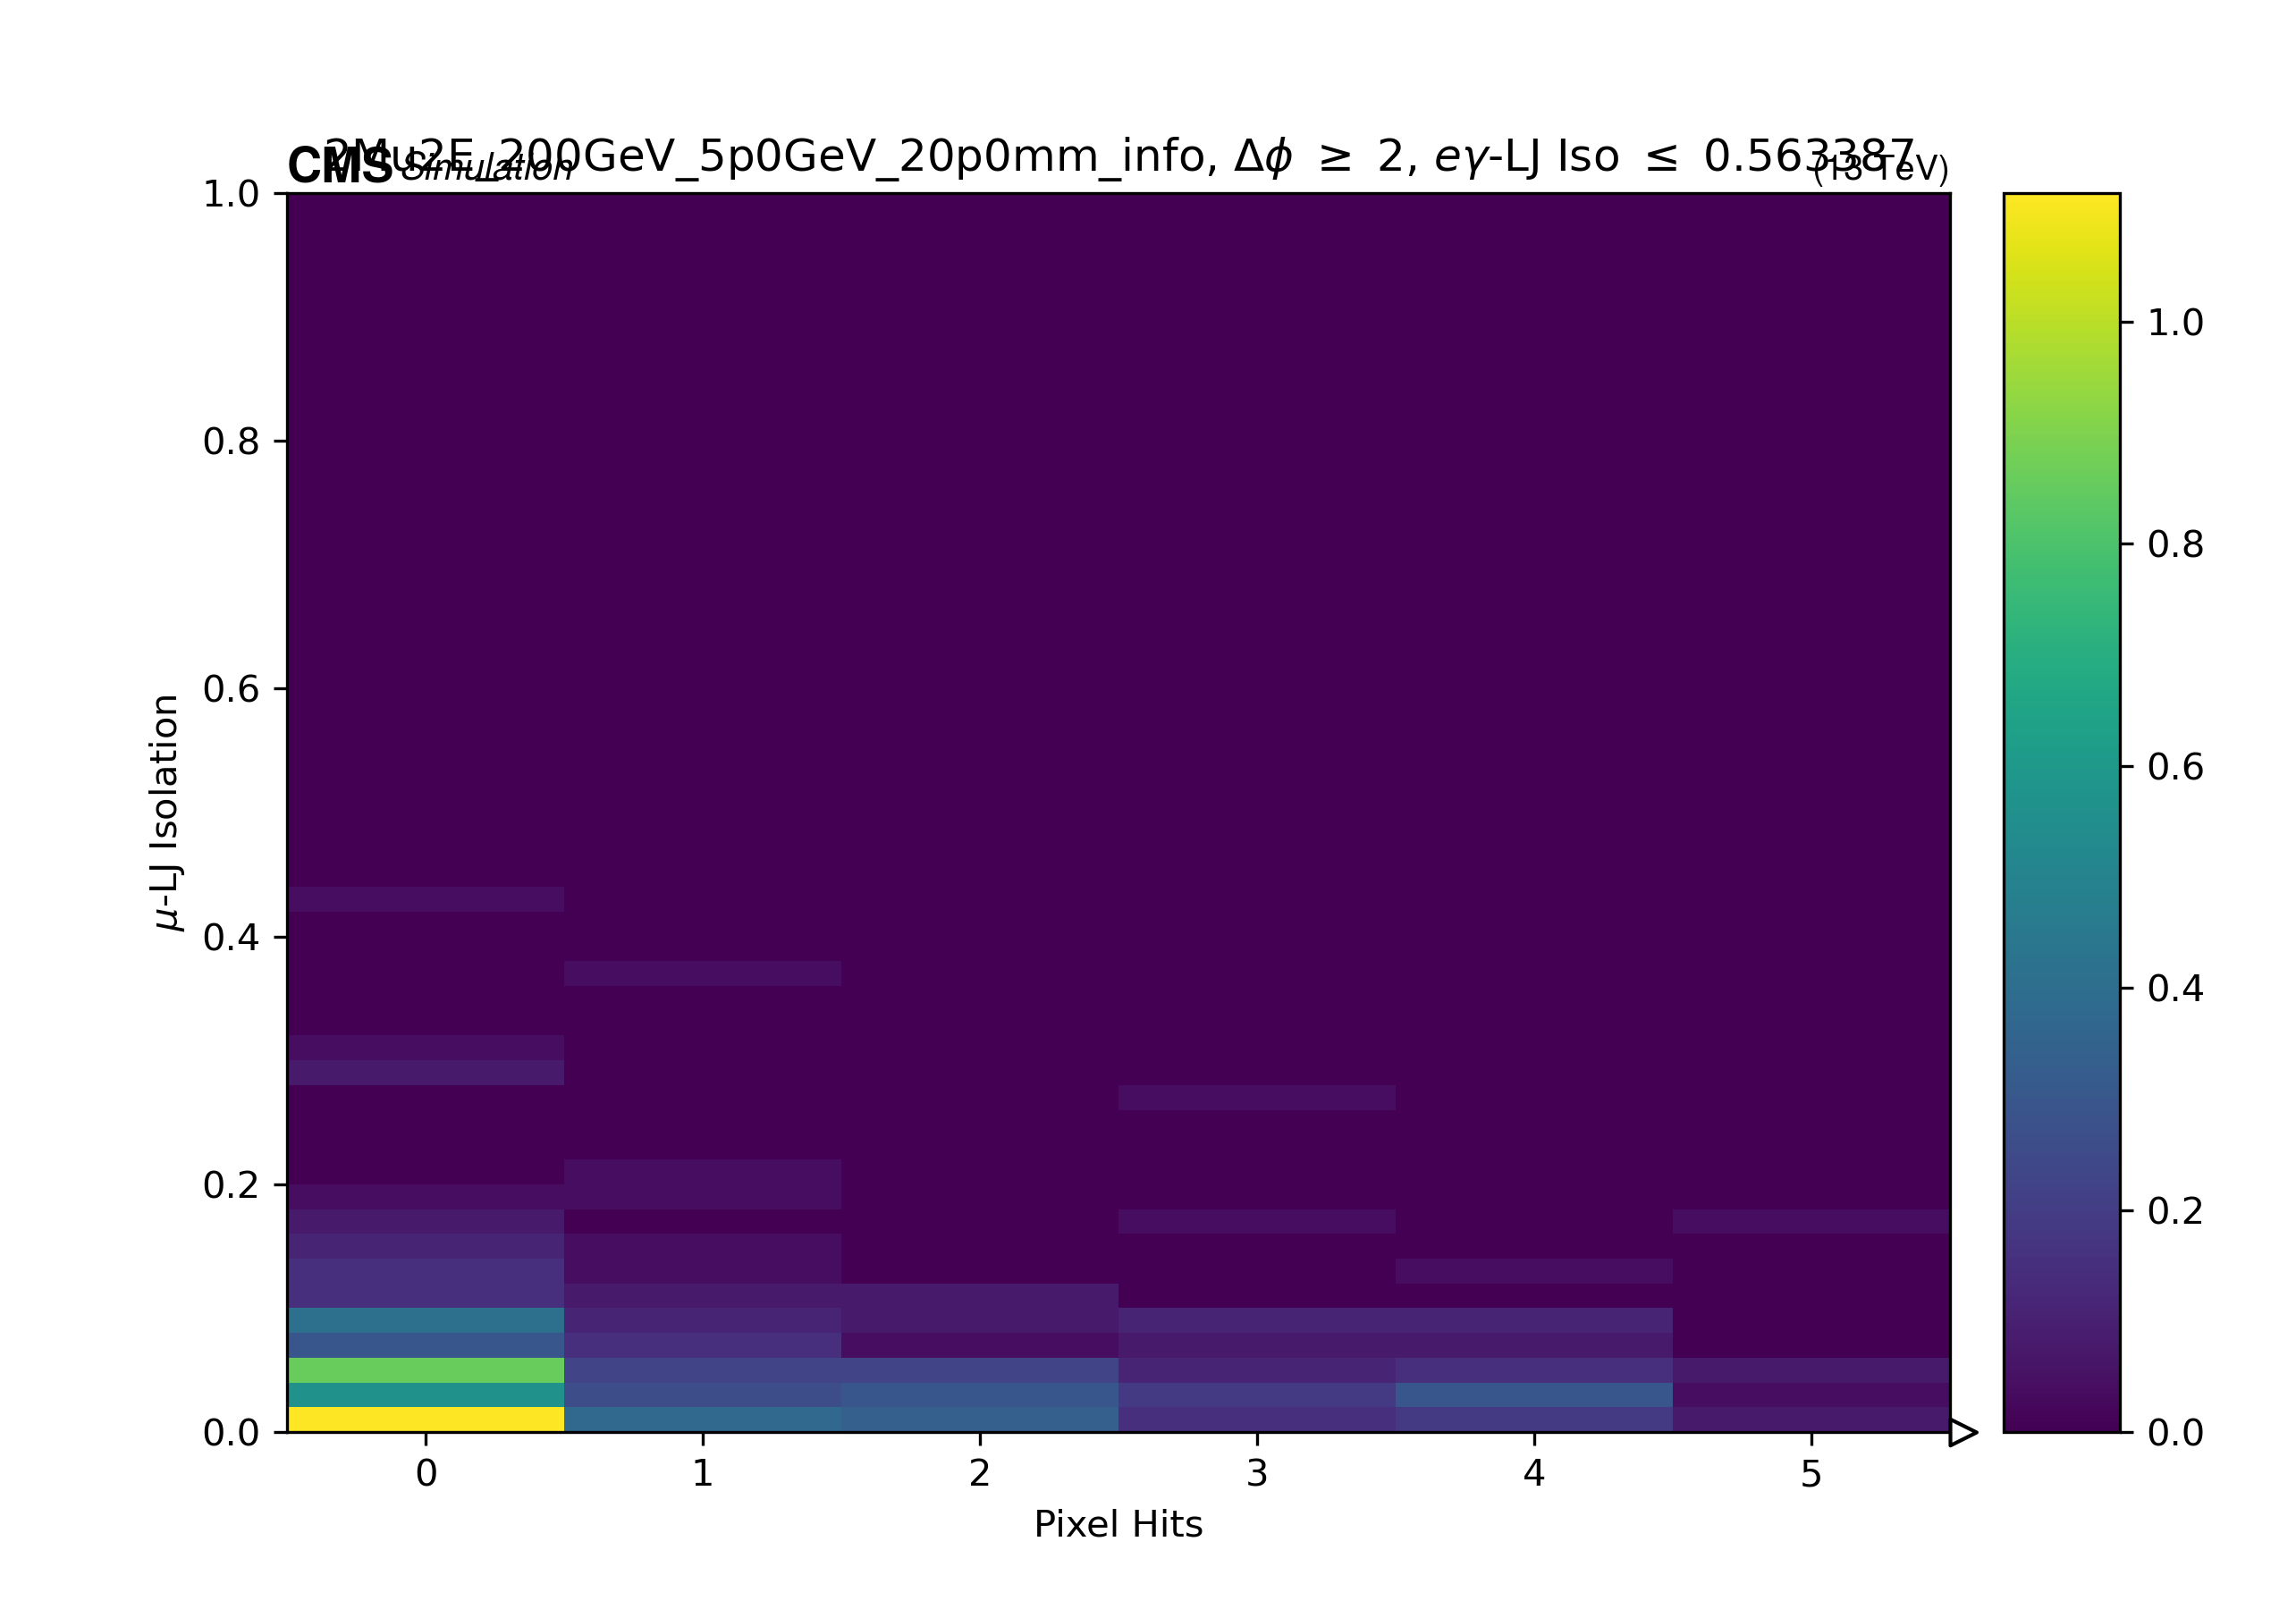
\includegraphics[width=\linewidth]{figures/2D_mJIso_vs_pixelHits_2Mu2E_200GeV_5p0GeV_20p0mm_info.png}
		\end{column}
	\end{columns}
\end{frame}

\begin{frame}{500 GeV}
	\centering
	\begin{columns}
		\begin{column}{0.333\textwidth}
			\centering
			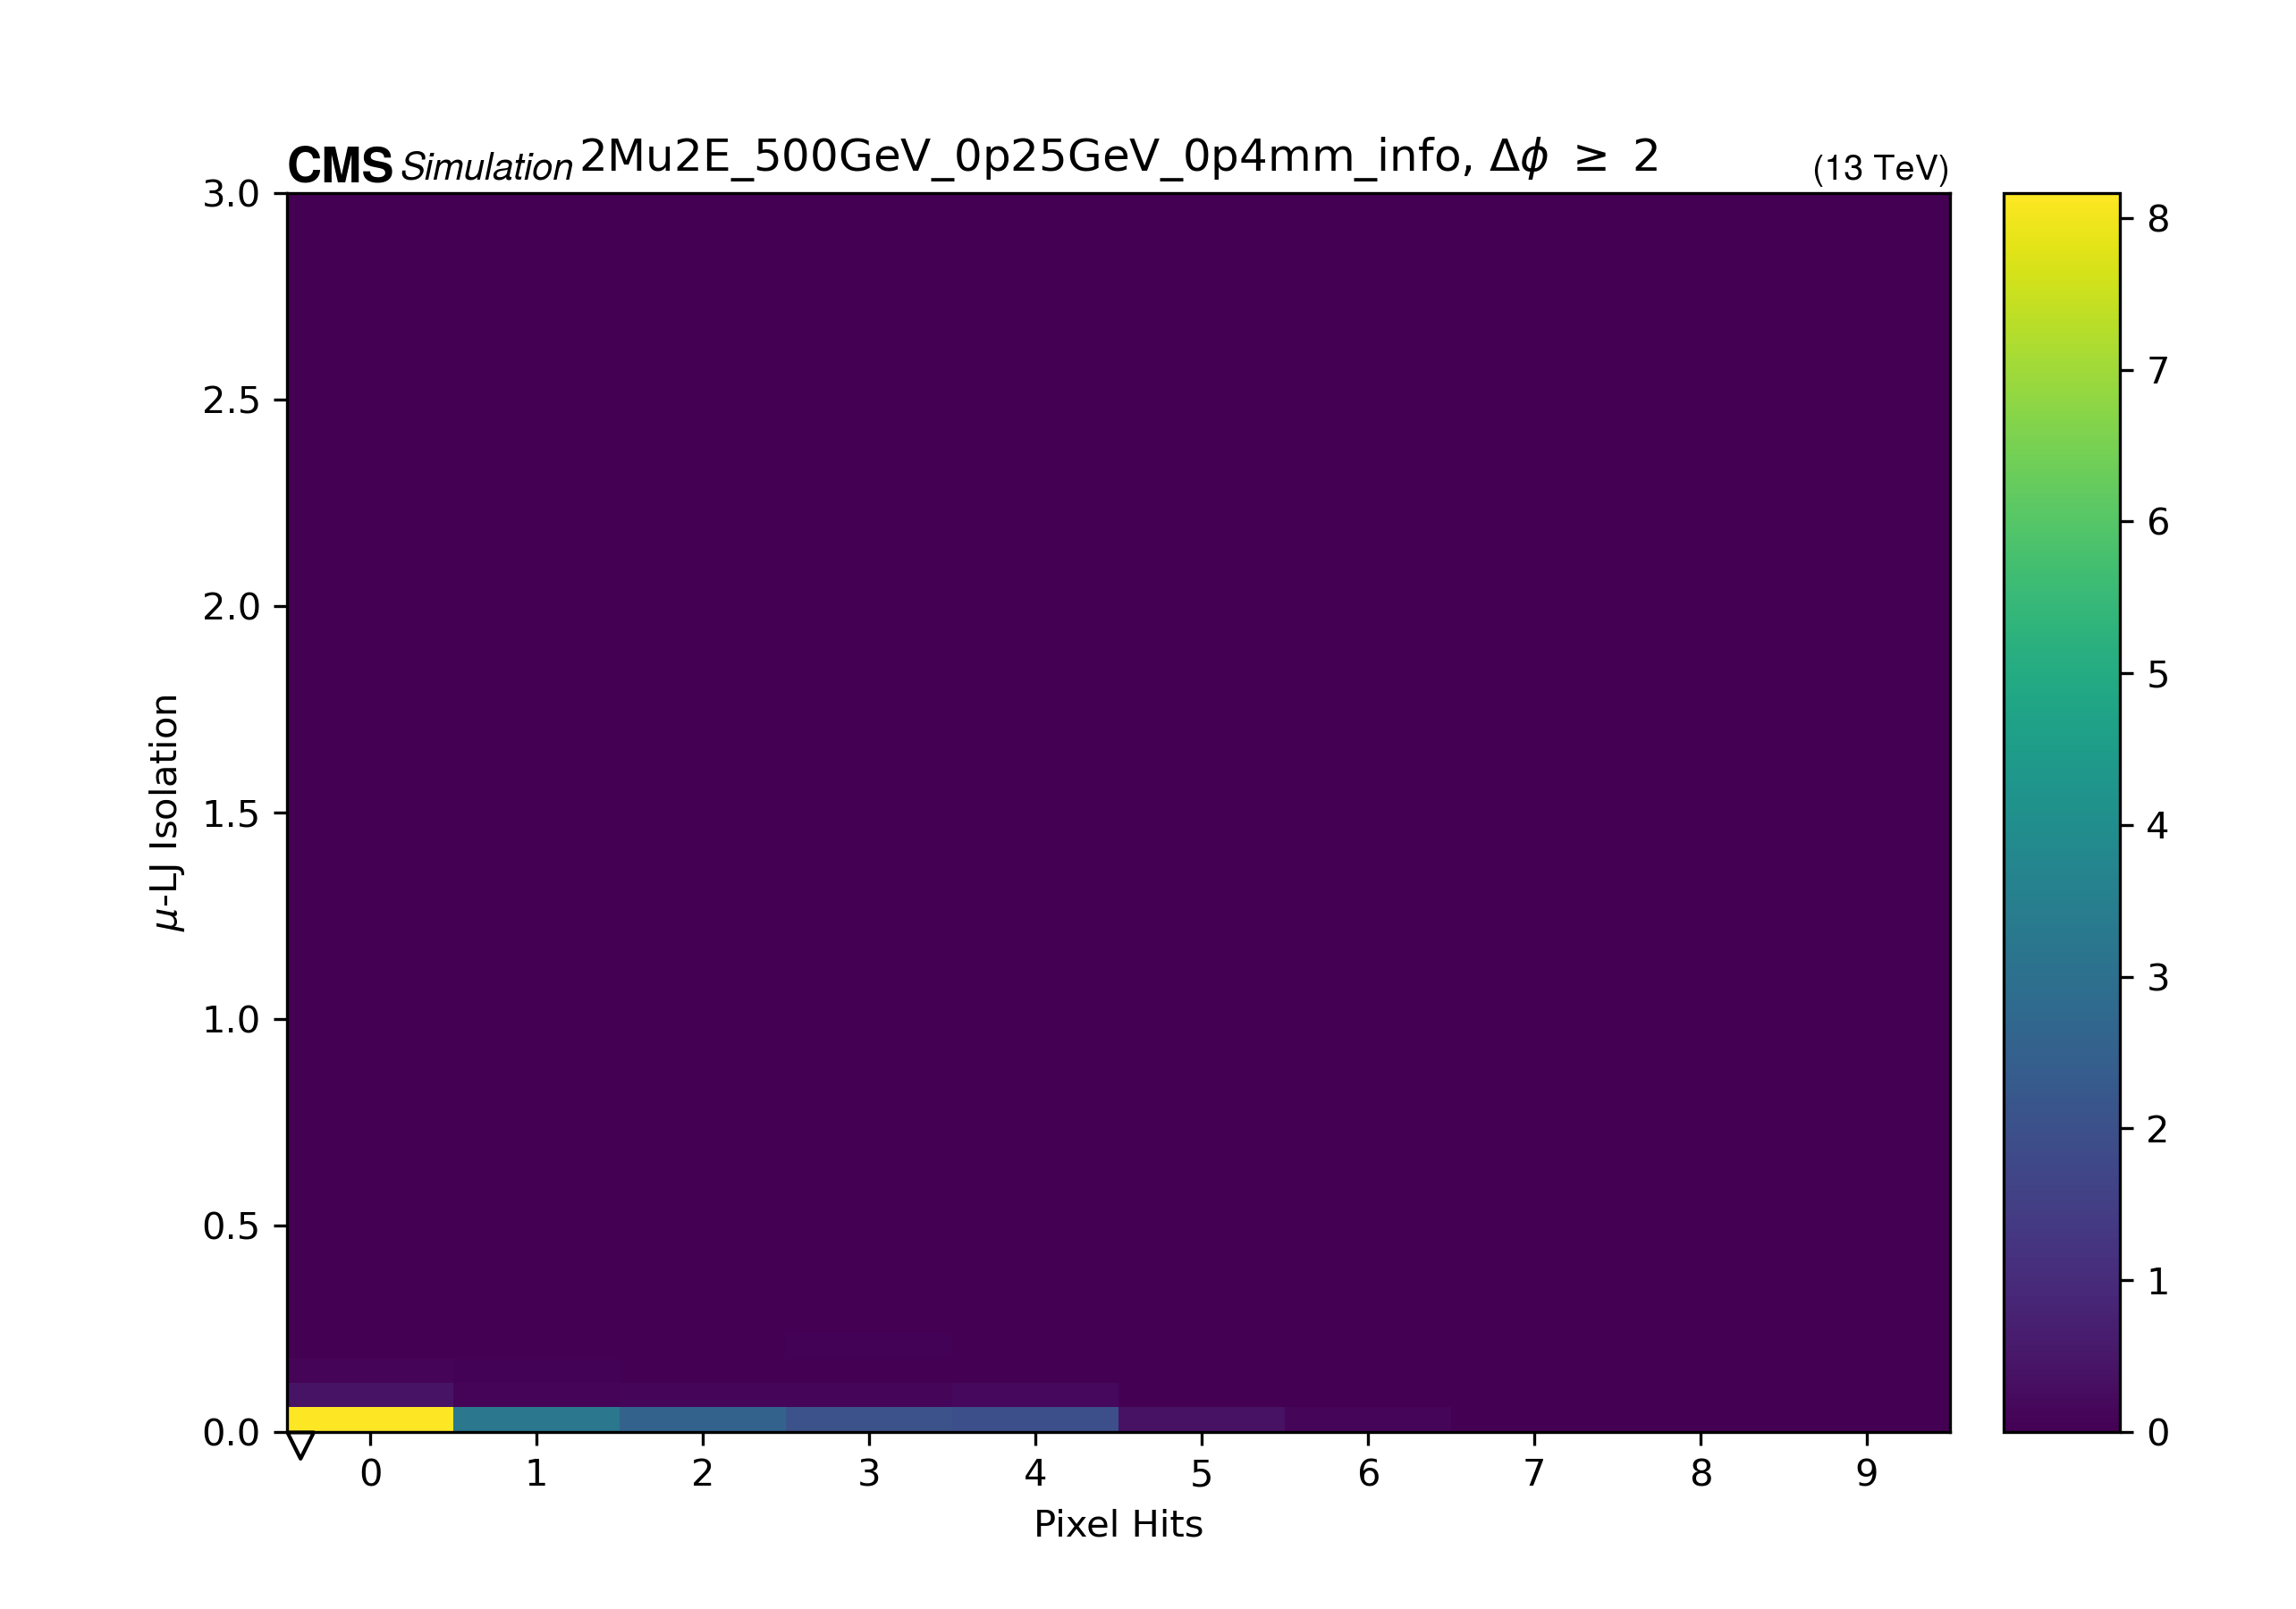
\includegraphics[width=\linewidth]{figures/2D_mJIso_vs_pixelHits_2Mu2E_500GeV_0p25GeV_0p4mm_info.png}
		\end{column}
		\begin{column}{0.333\textwidth}
			\centering
			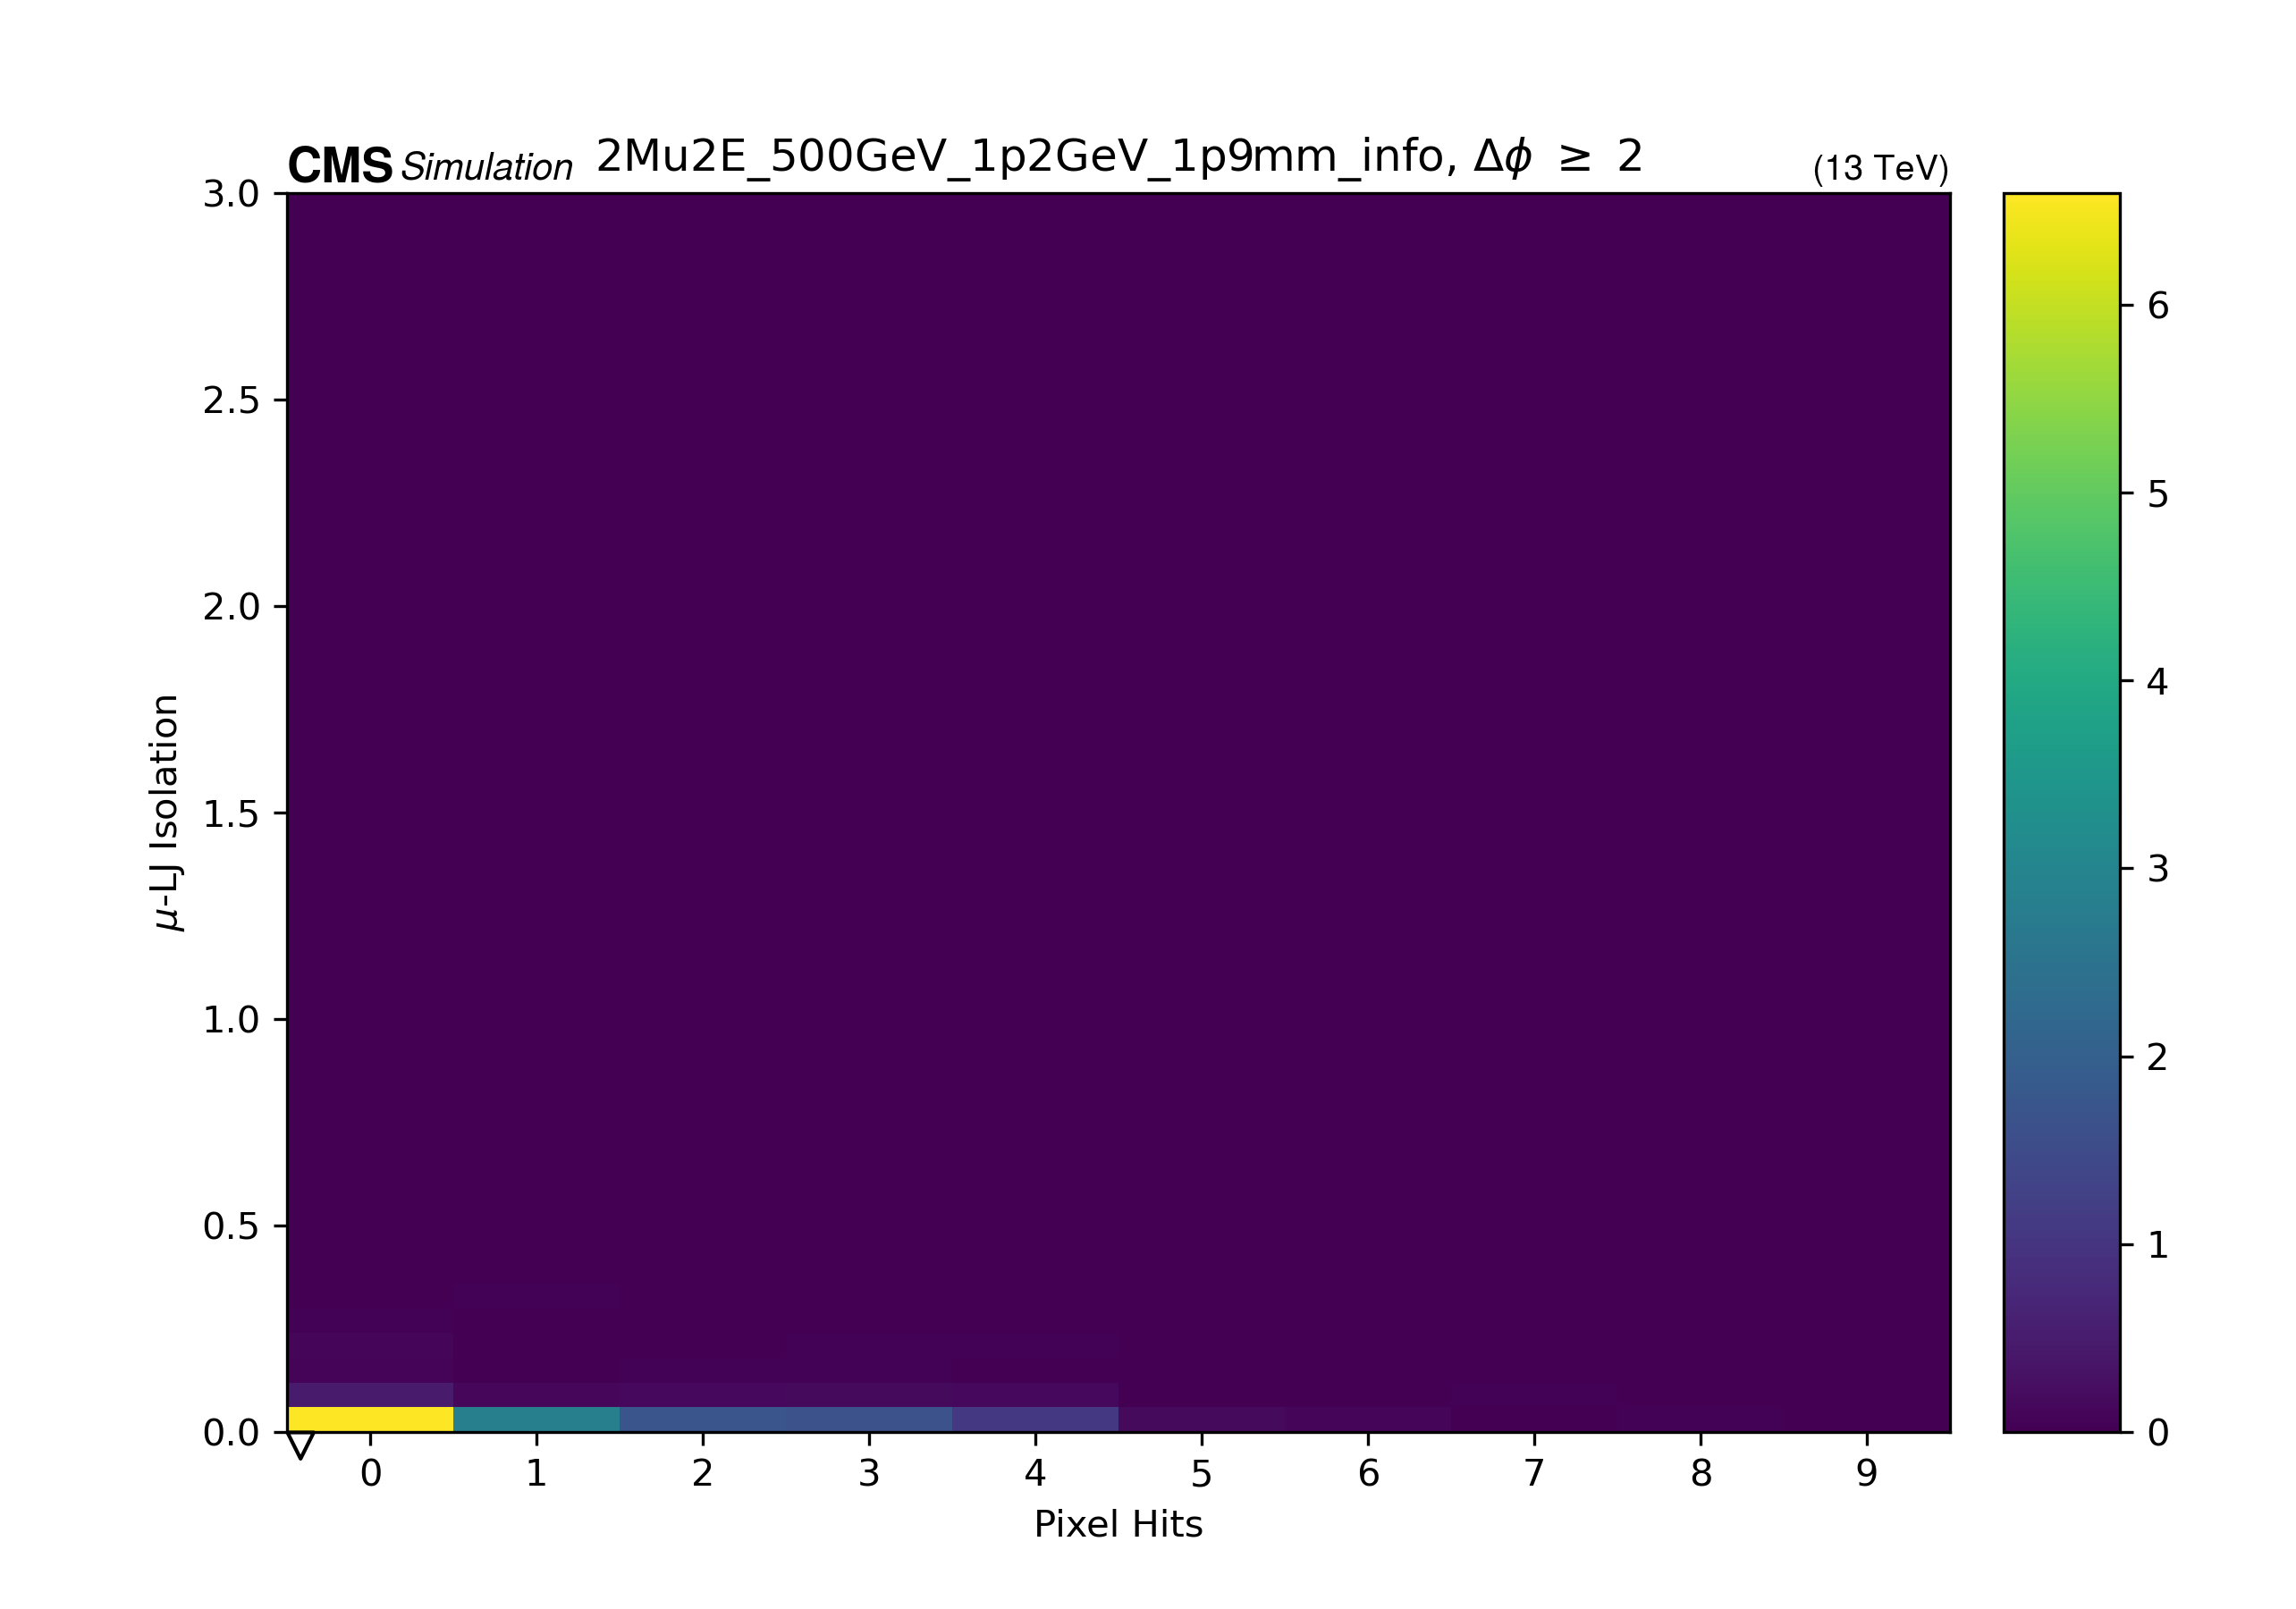
\includegraphics[width=\linewidth]{figures/2D_mJIso_vs_pixelHits_2Mu2E_500GeV_1p2GeV_1p9mm_info.png}
		\end{column}
		\begin{column}{0.333\textwidth}
			\centering
			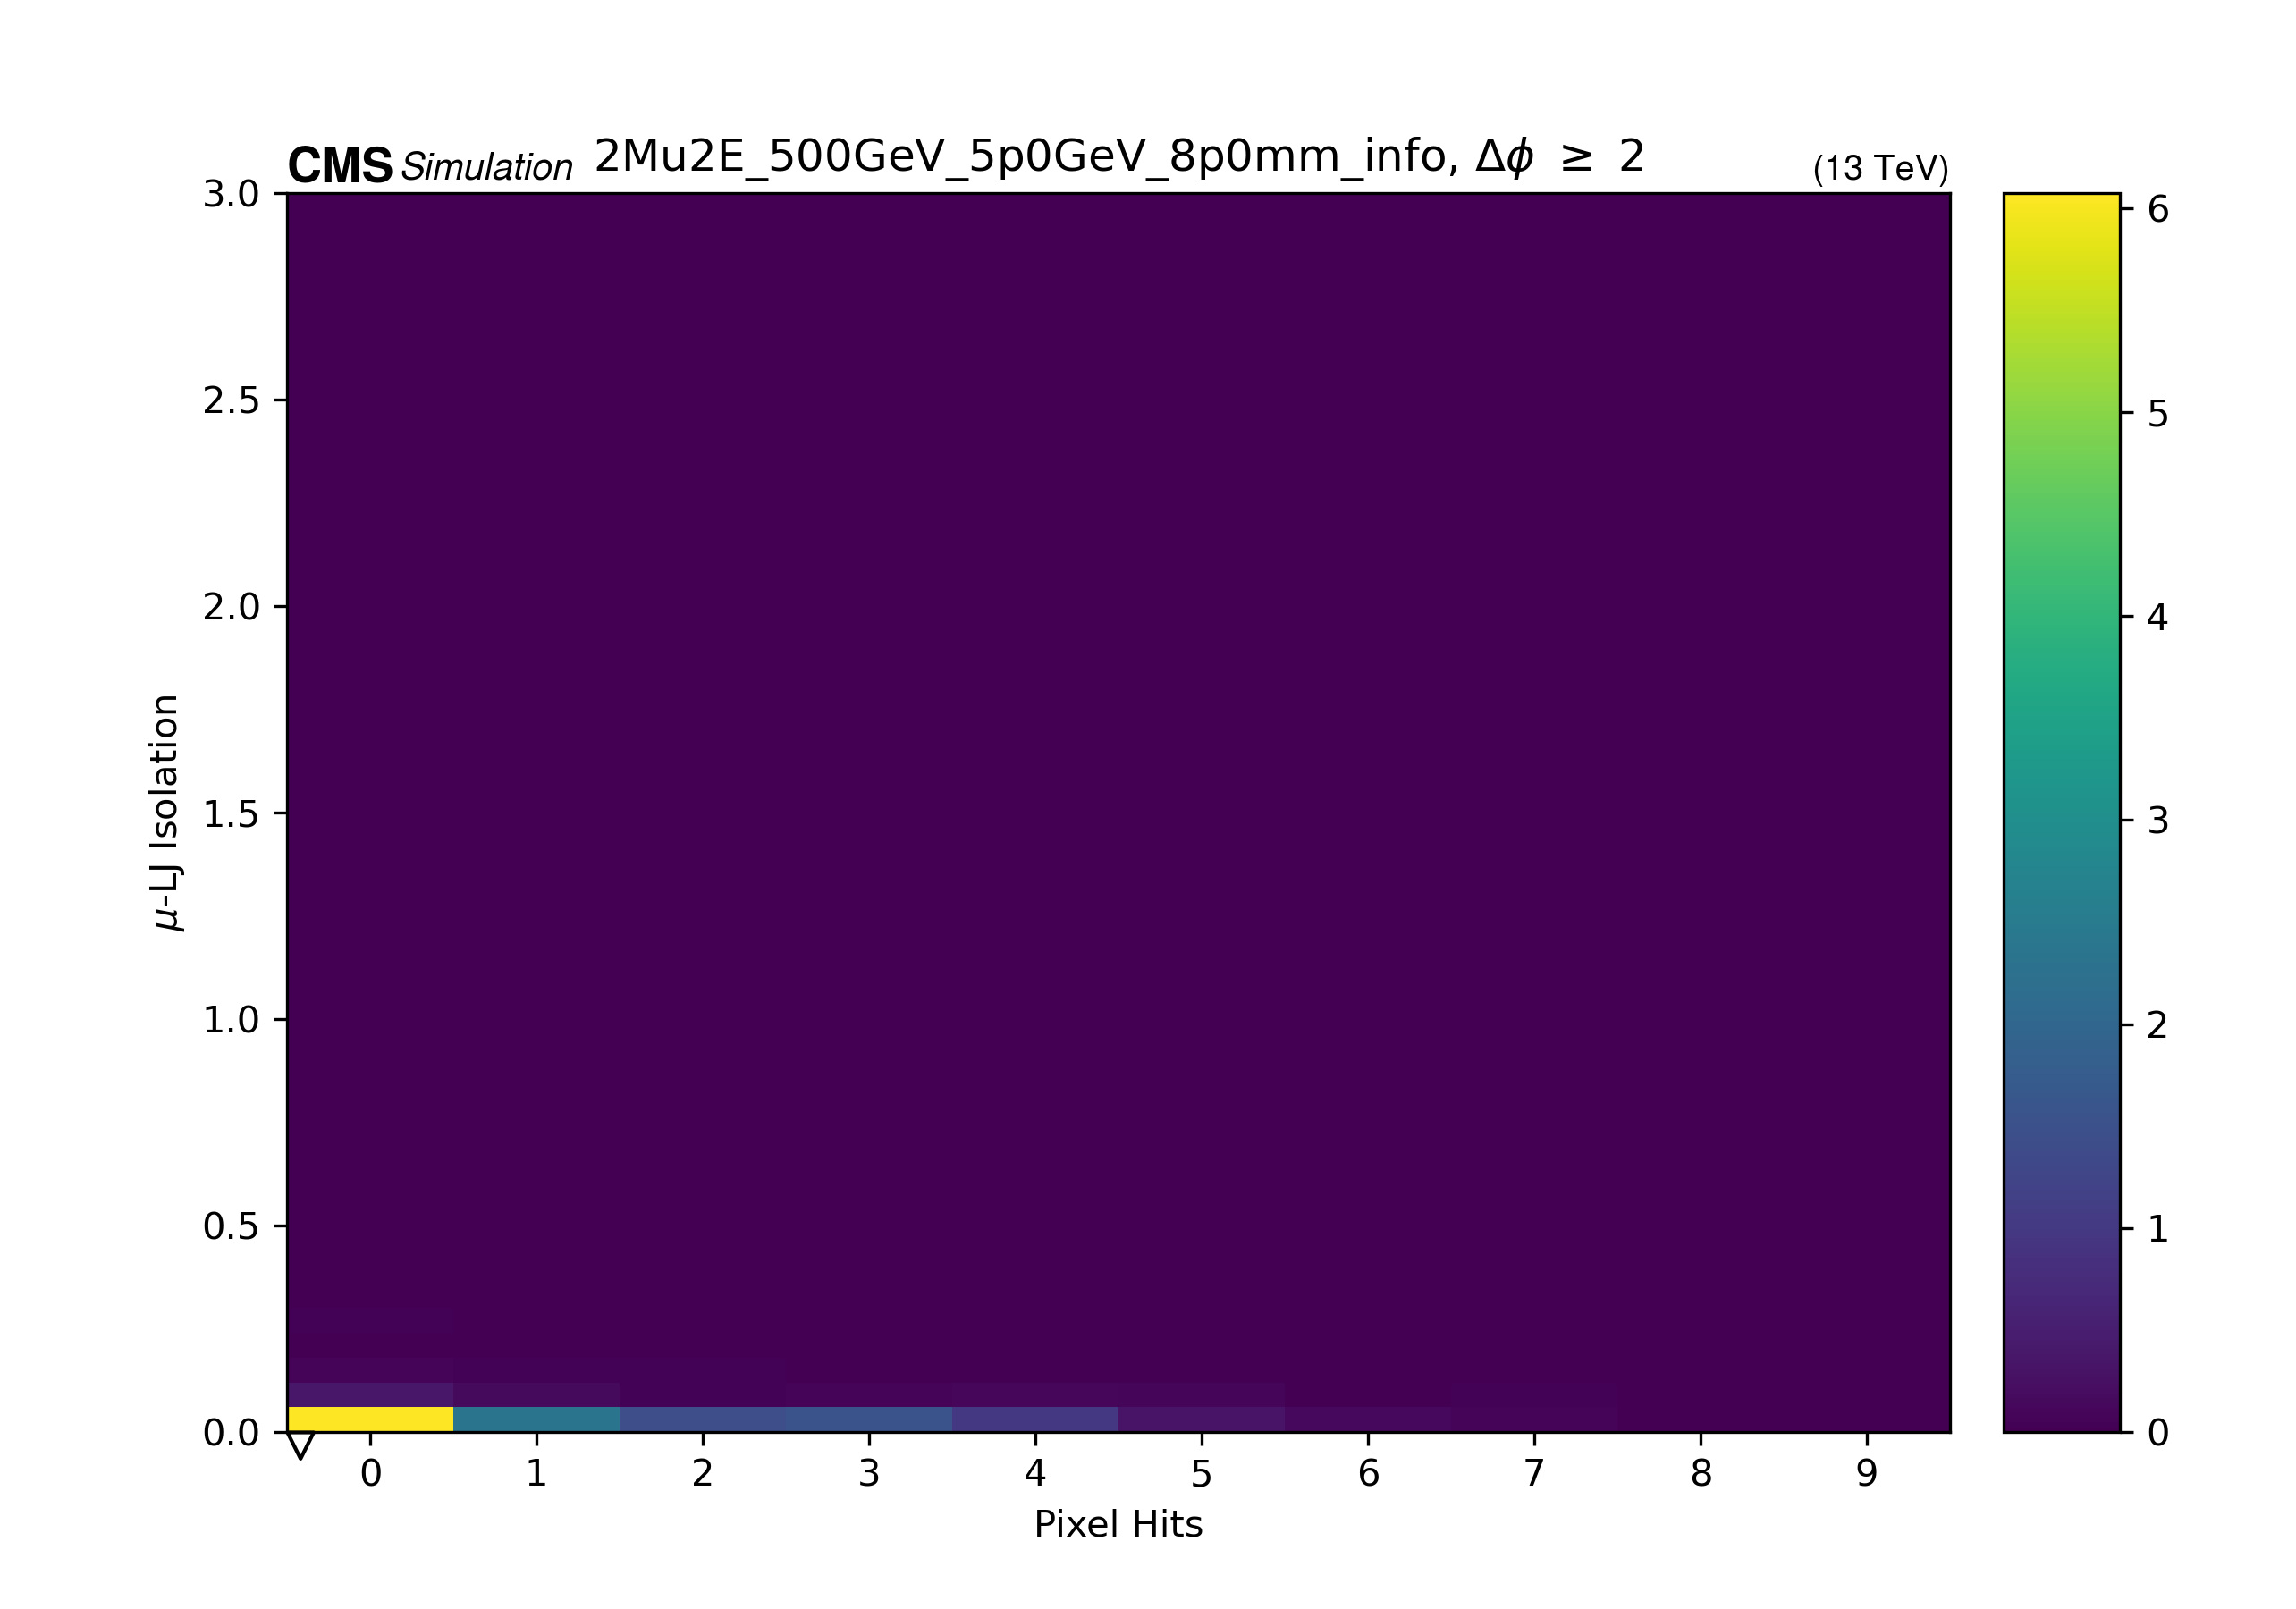
\includegraphics[width=\linewidth]{figures/2D_mJIso_vs_pixelHits_2Mu2E_500GeV_5p0GeV_8p0mm_info.png}
		\end{column}
	\end{columns}
\end{frame}

\begin{frame}{800 GeV}
	\centering
	\begin{columns}
		\begin{column}{0.333\textwidth}
			\centering
			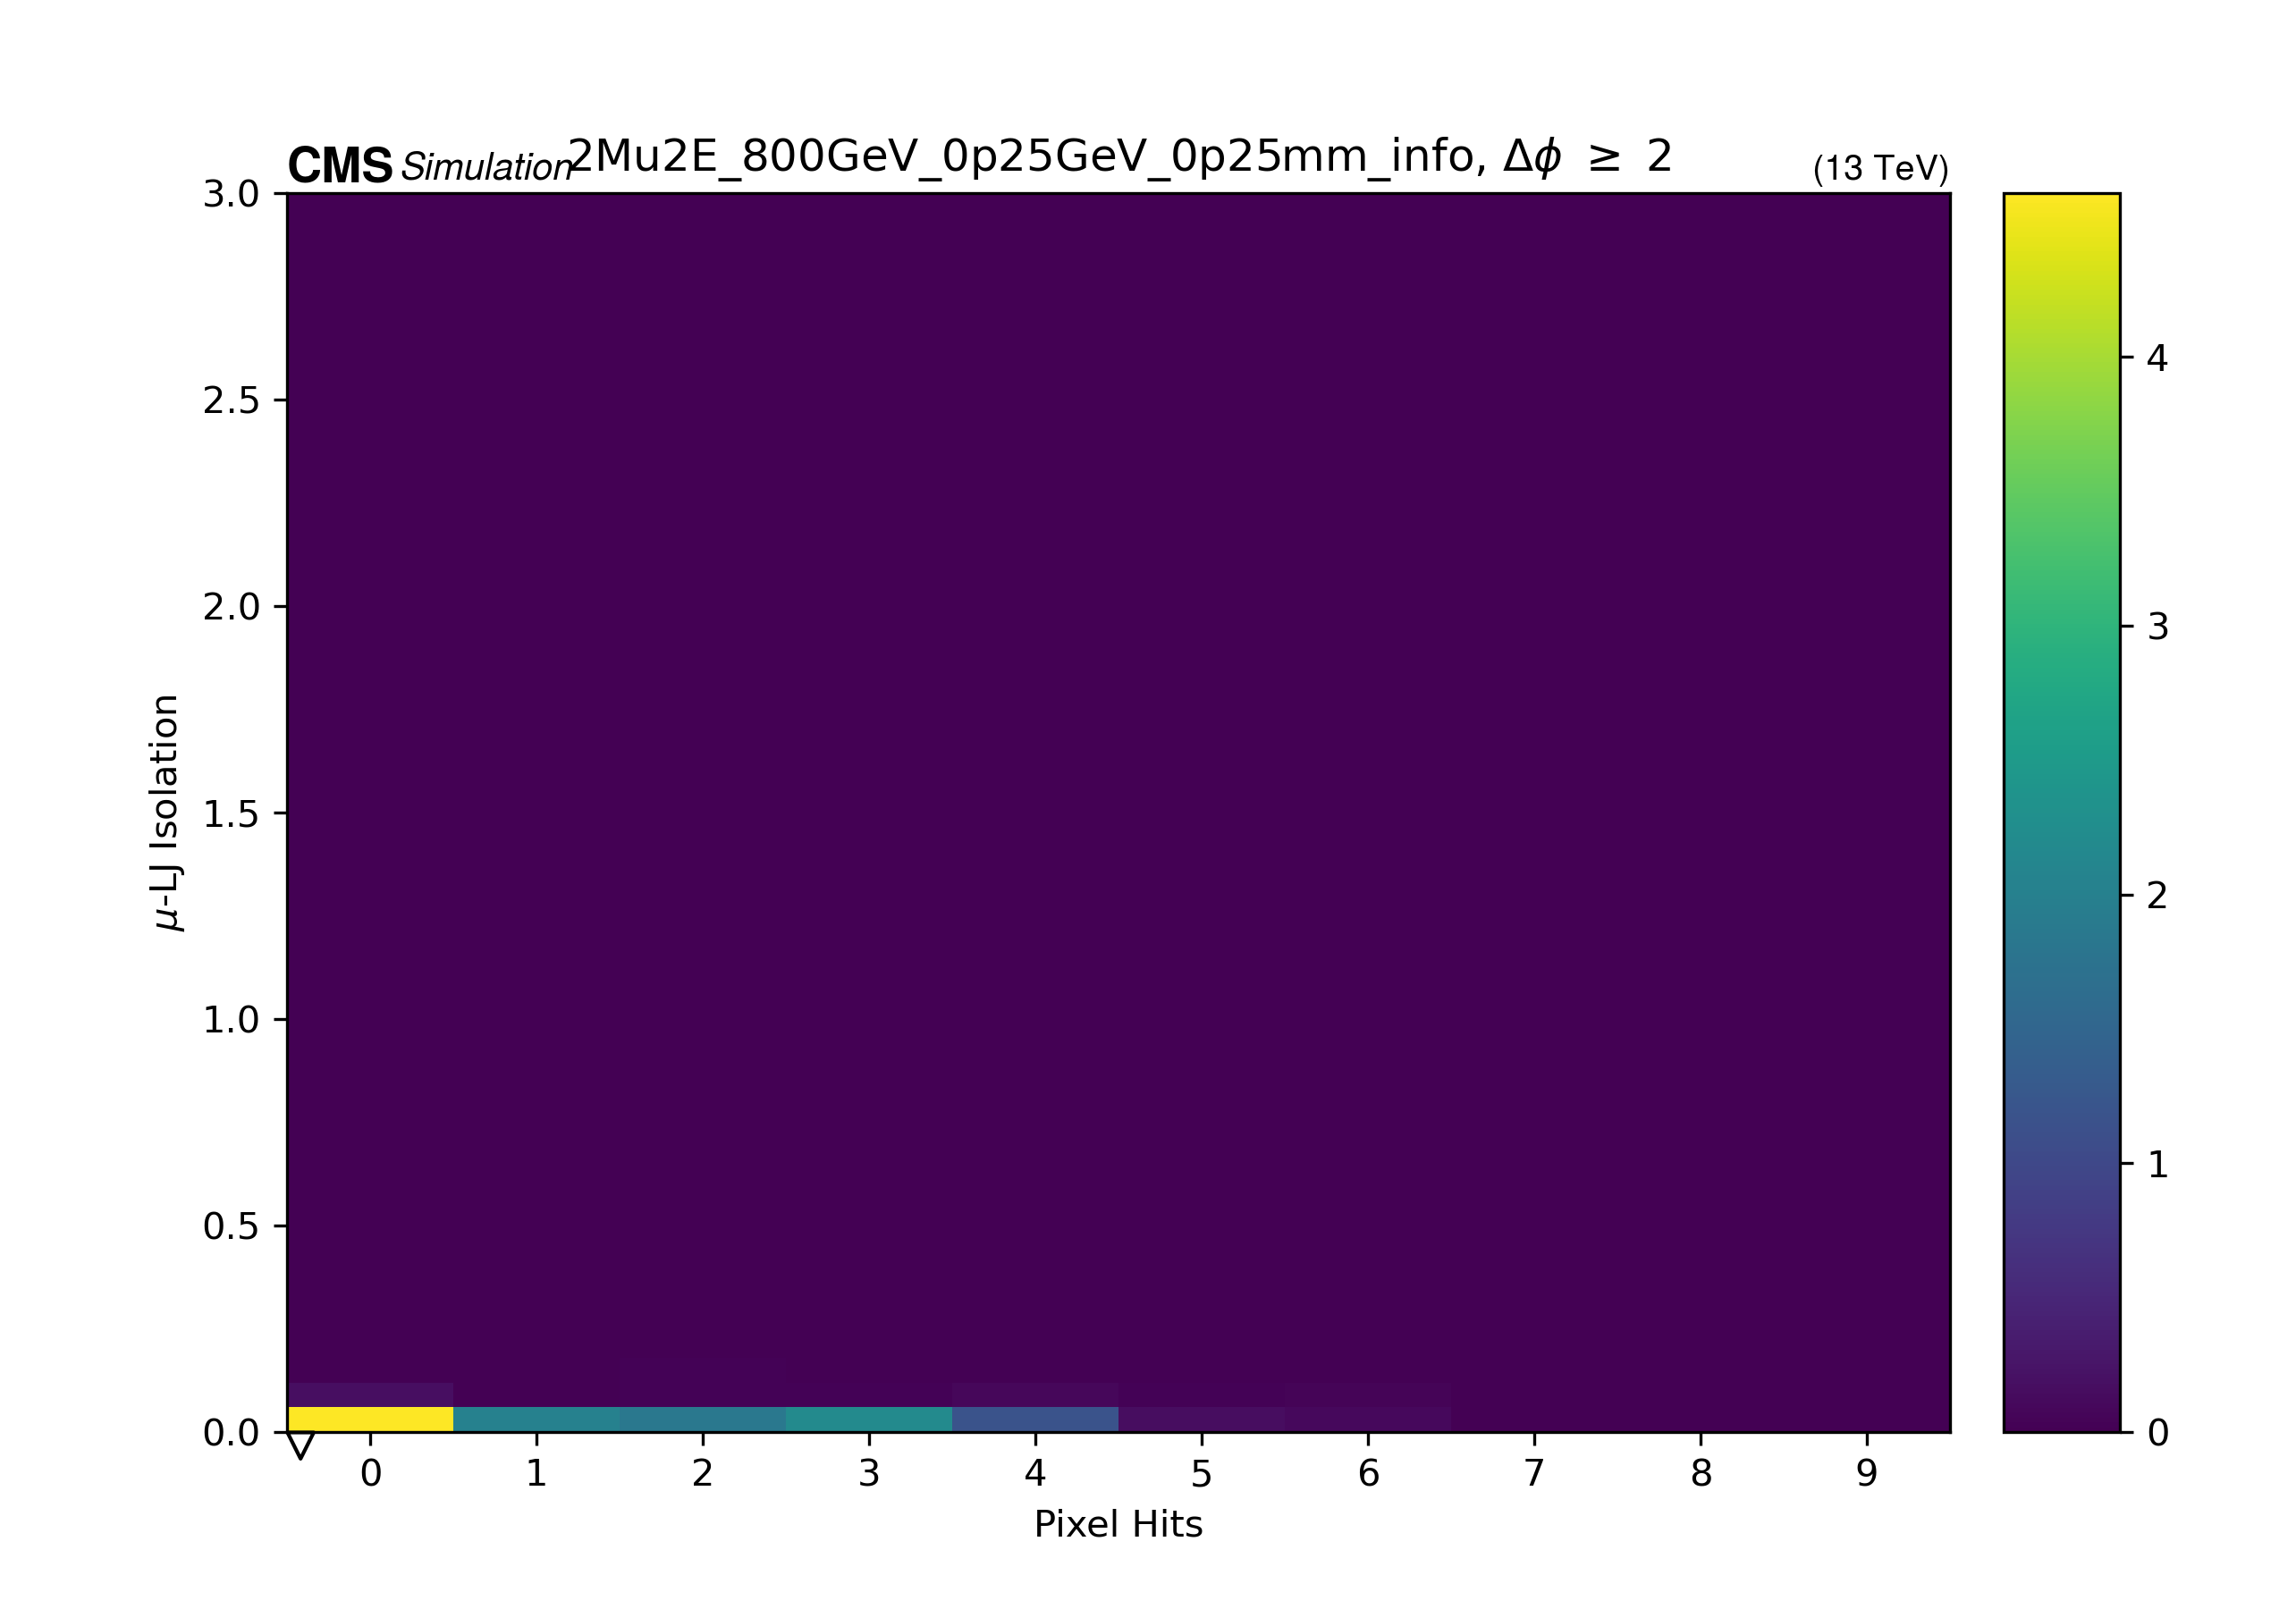
\includegraphics[width=\linewidth]{figures/2D_mJIso_vs_pixelHits_2Mu2E_800GeV_0p25GeV_0p25mm_info.png}
		\end{column}
		\begin{column}{0.333\textwidth}
			\centering
			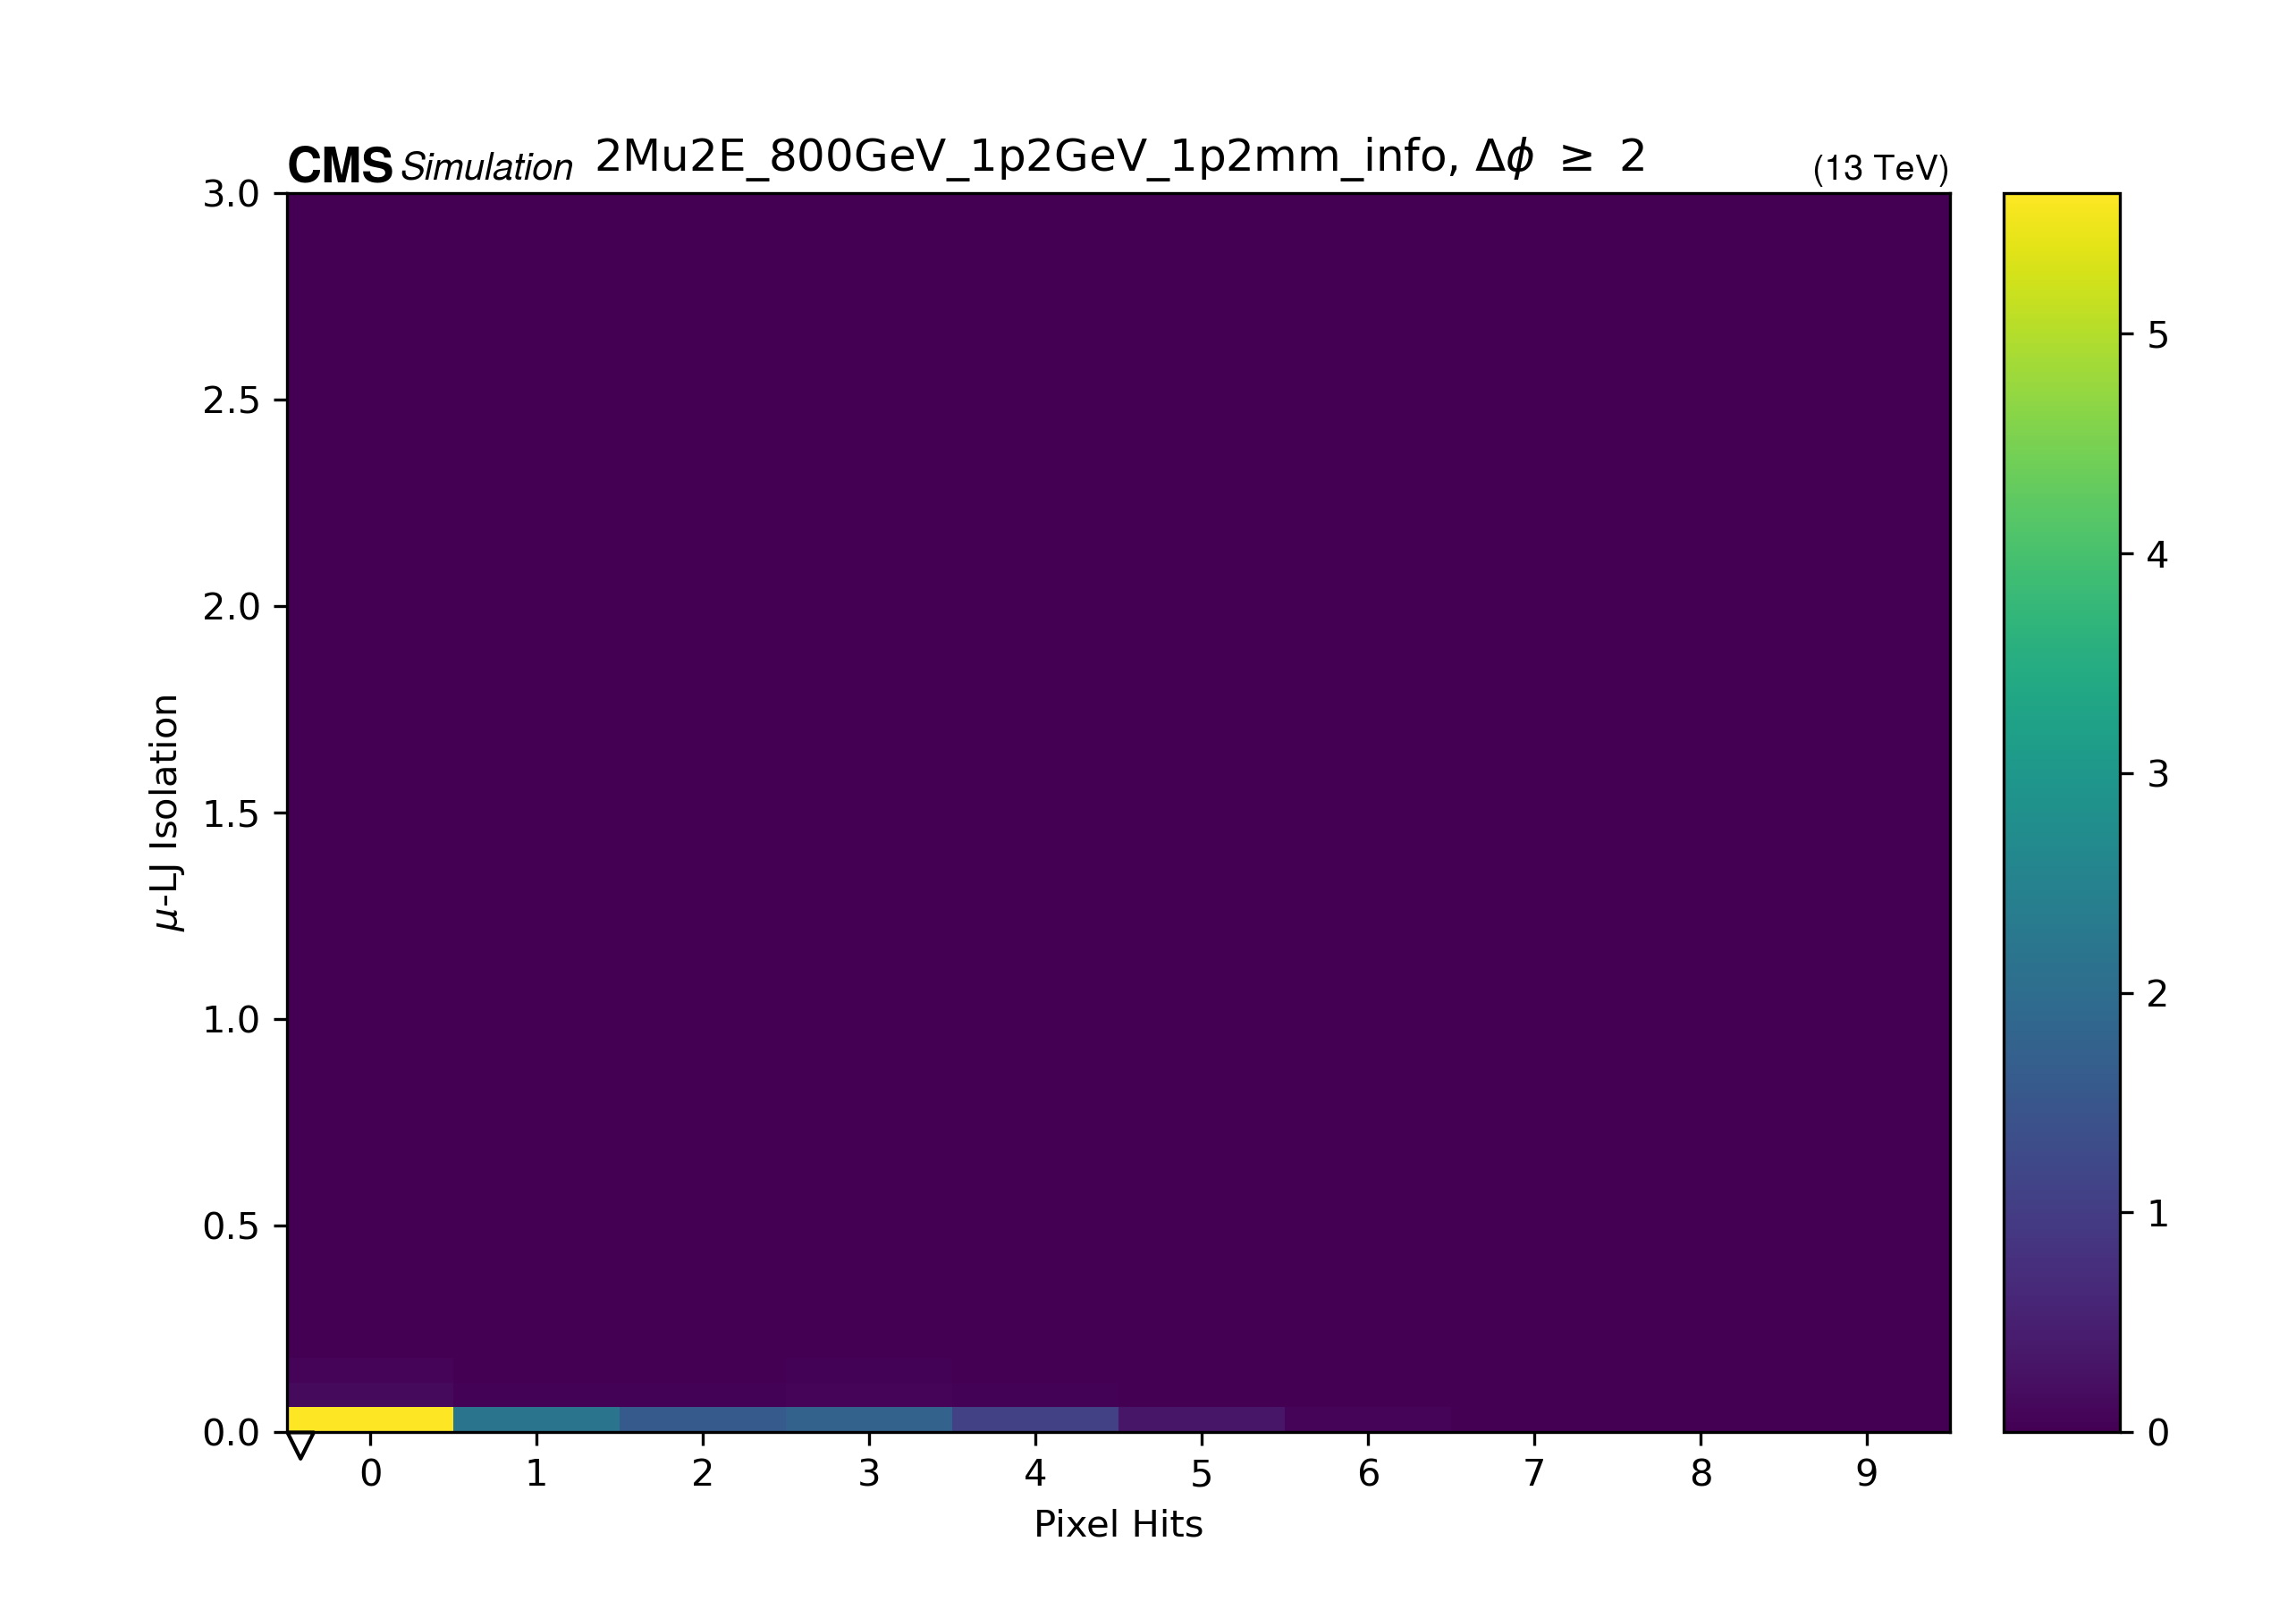
\includegraphics[width=\linewidth]{figures/2D_mJIso_vs_pixelHits_2Mu2E_800GeV_1p2GeV_1p2mm_info.png}
		\end{column}
		\begin{column}{0.333\textwidth}
			\centering
			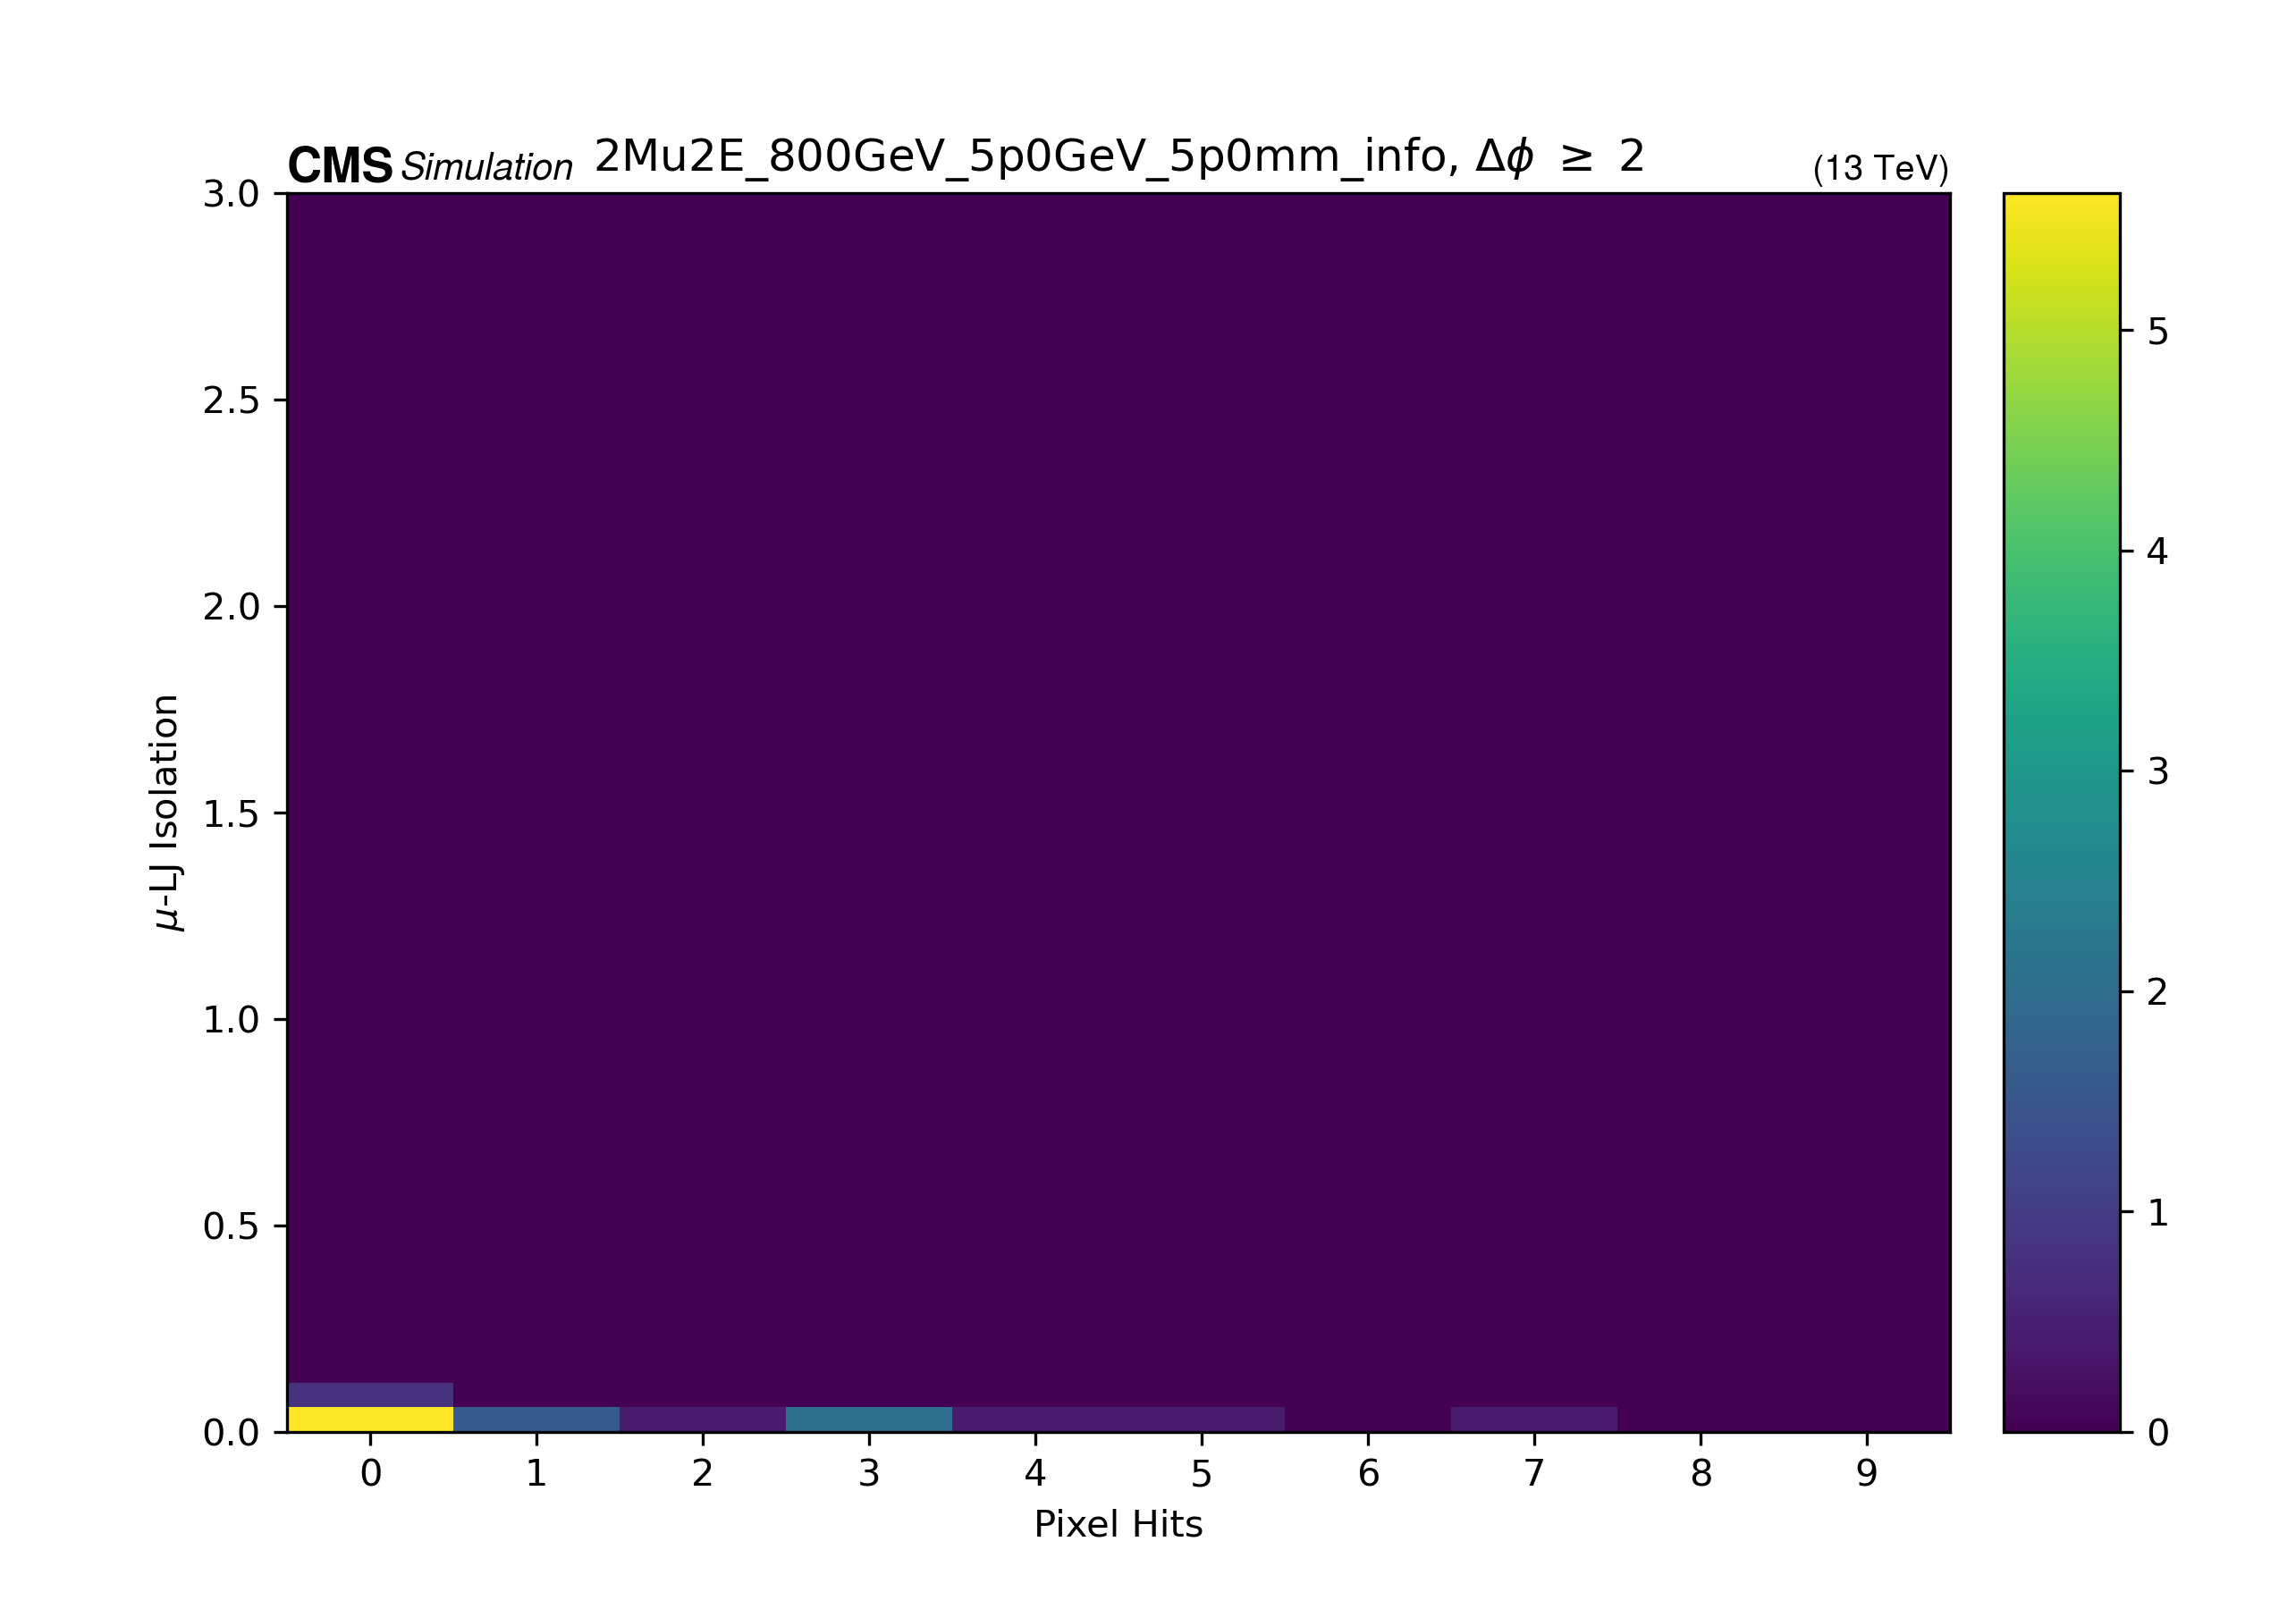
\includegraphics[width=\linewidth]{figures/2D_mJIso_vs_pixelHits_2Mu2E_800GeV_5p0GeV_5p0mm_info.png}
		\end{column}
	\end{columns}
\end{frame}

\begin{frame}{1000 GeV}
	\centering
	\begin{columns}
		\begin{column}{0.333\textwidth}
			\centering
			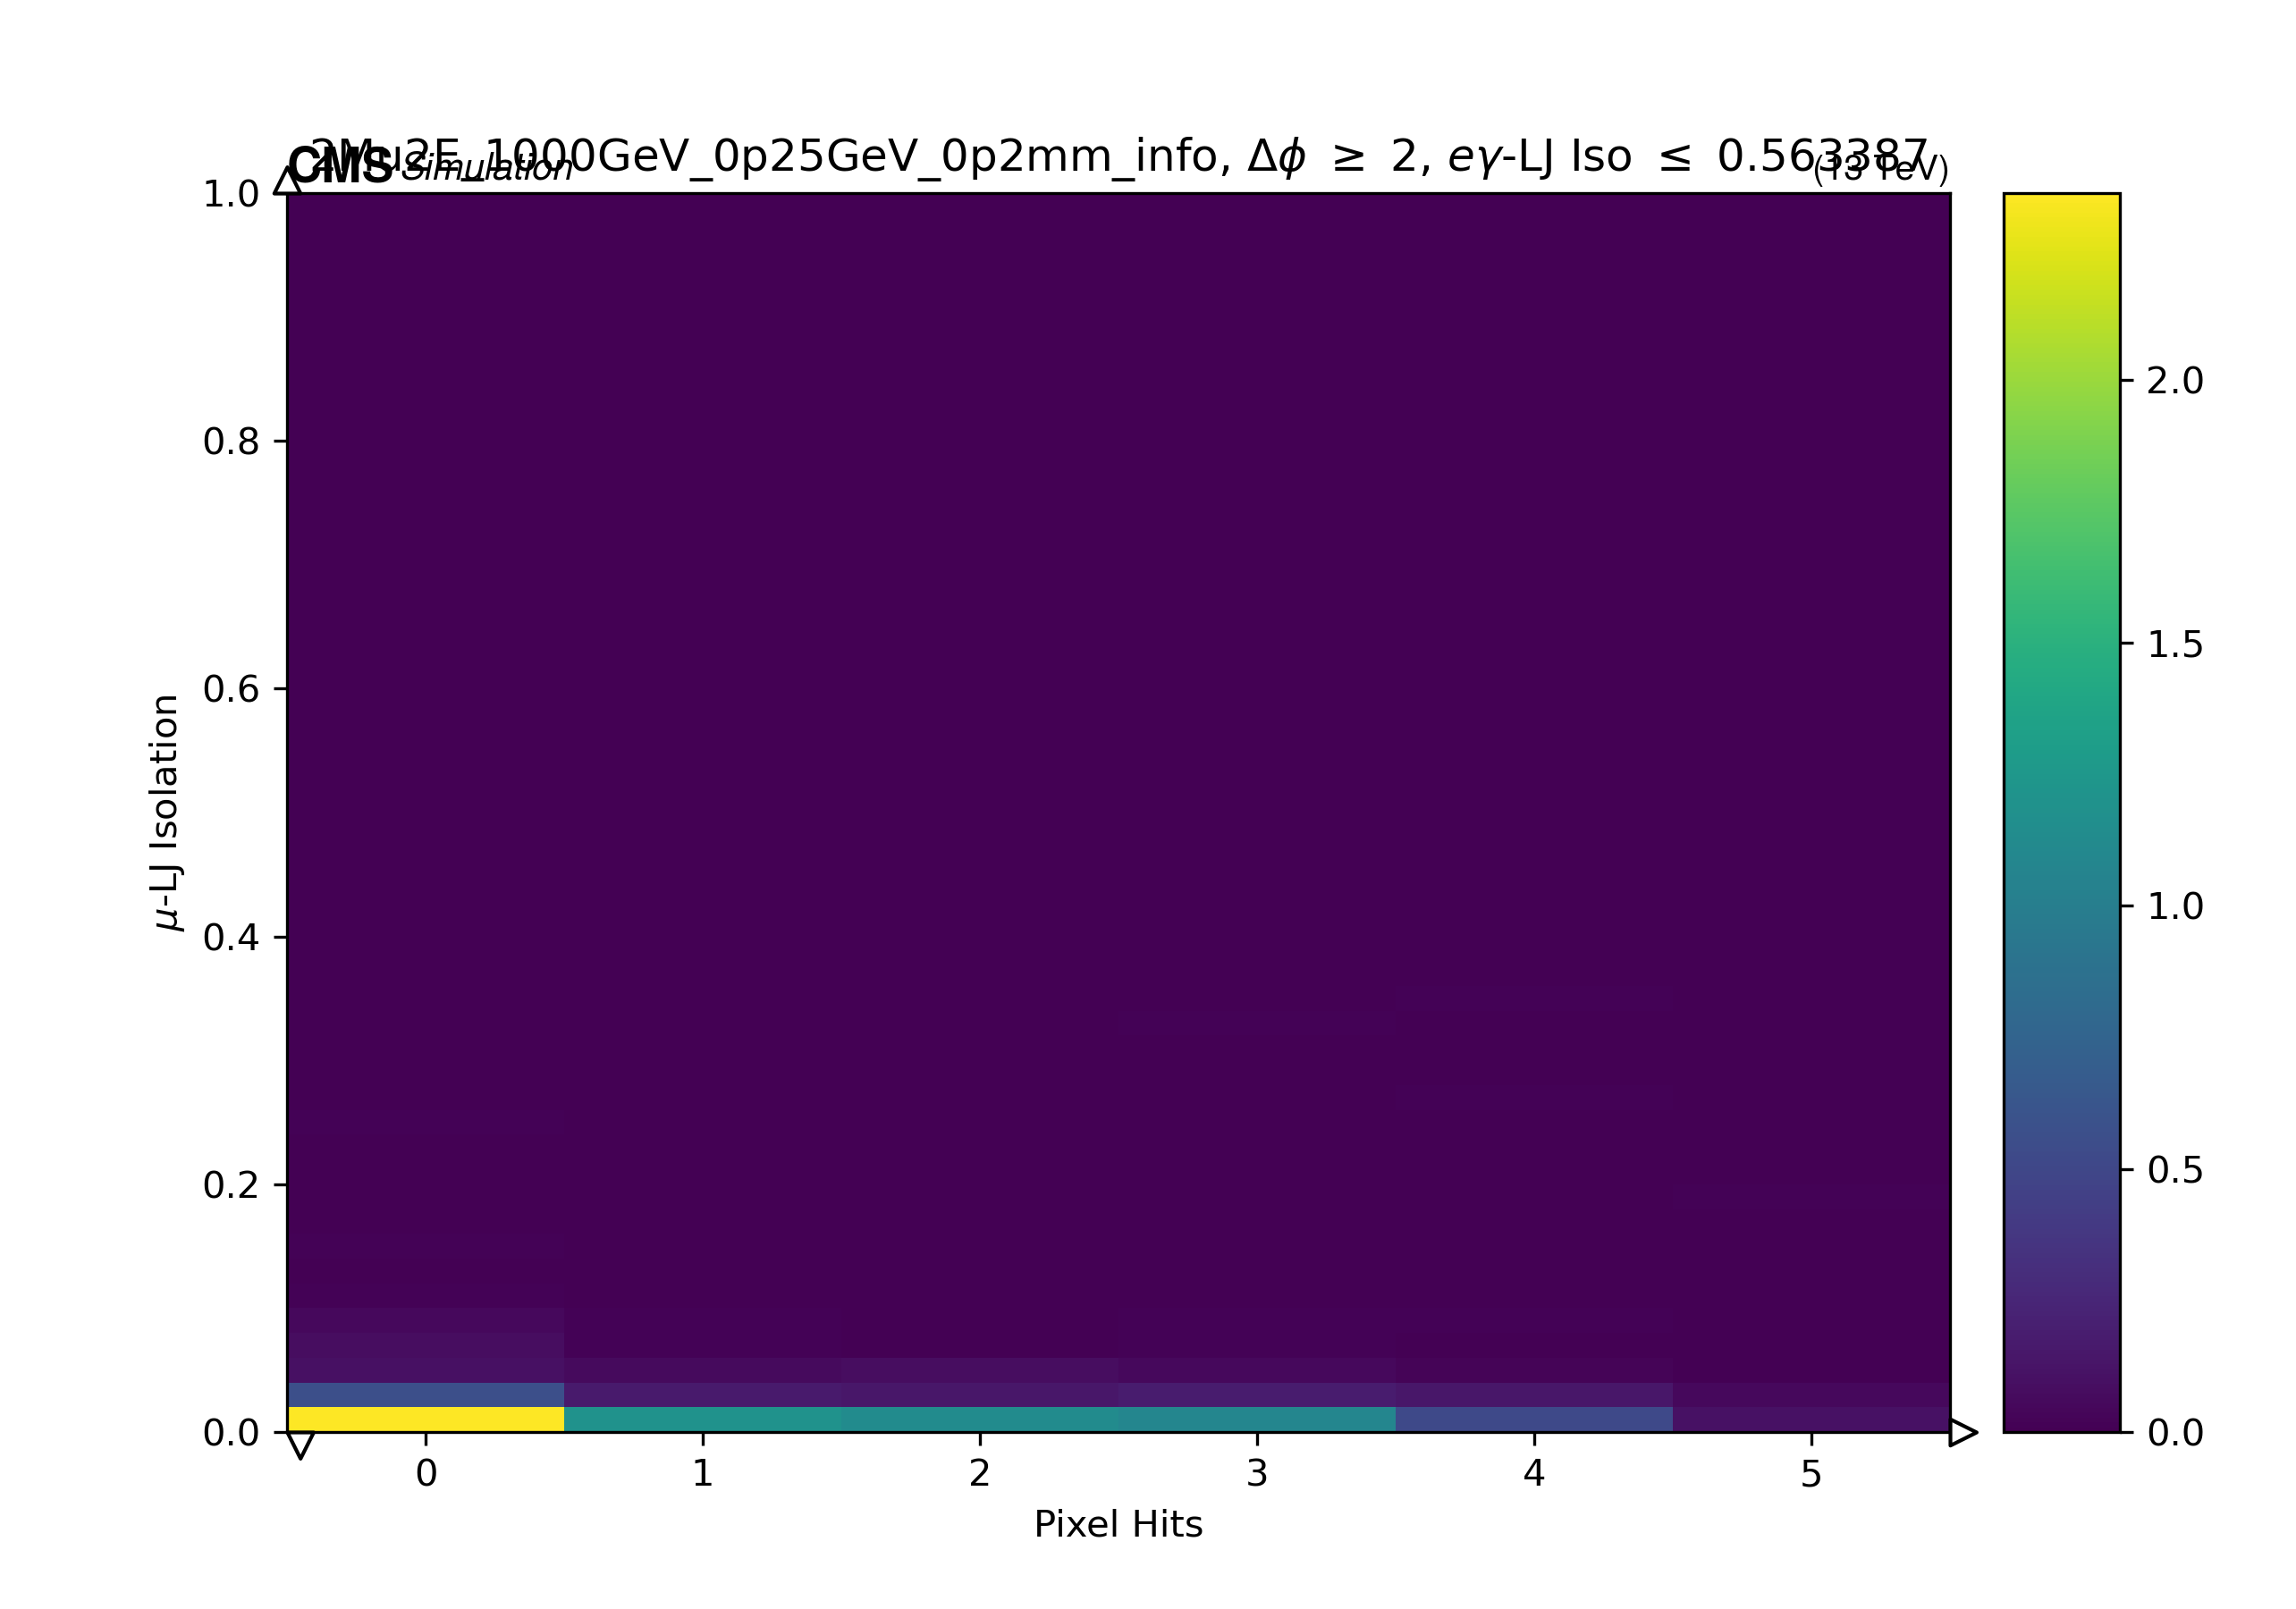
\includegraphics[width=\linewidth]{figures/2D_mJIso_vs_pixelHits_2Mu2E_1000GeV_0p25GeV_0p2mm_info.png}
		\end{column}
		\begin{column}{0.333\textwidth}
			\centering
			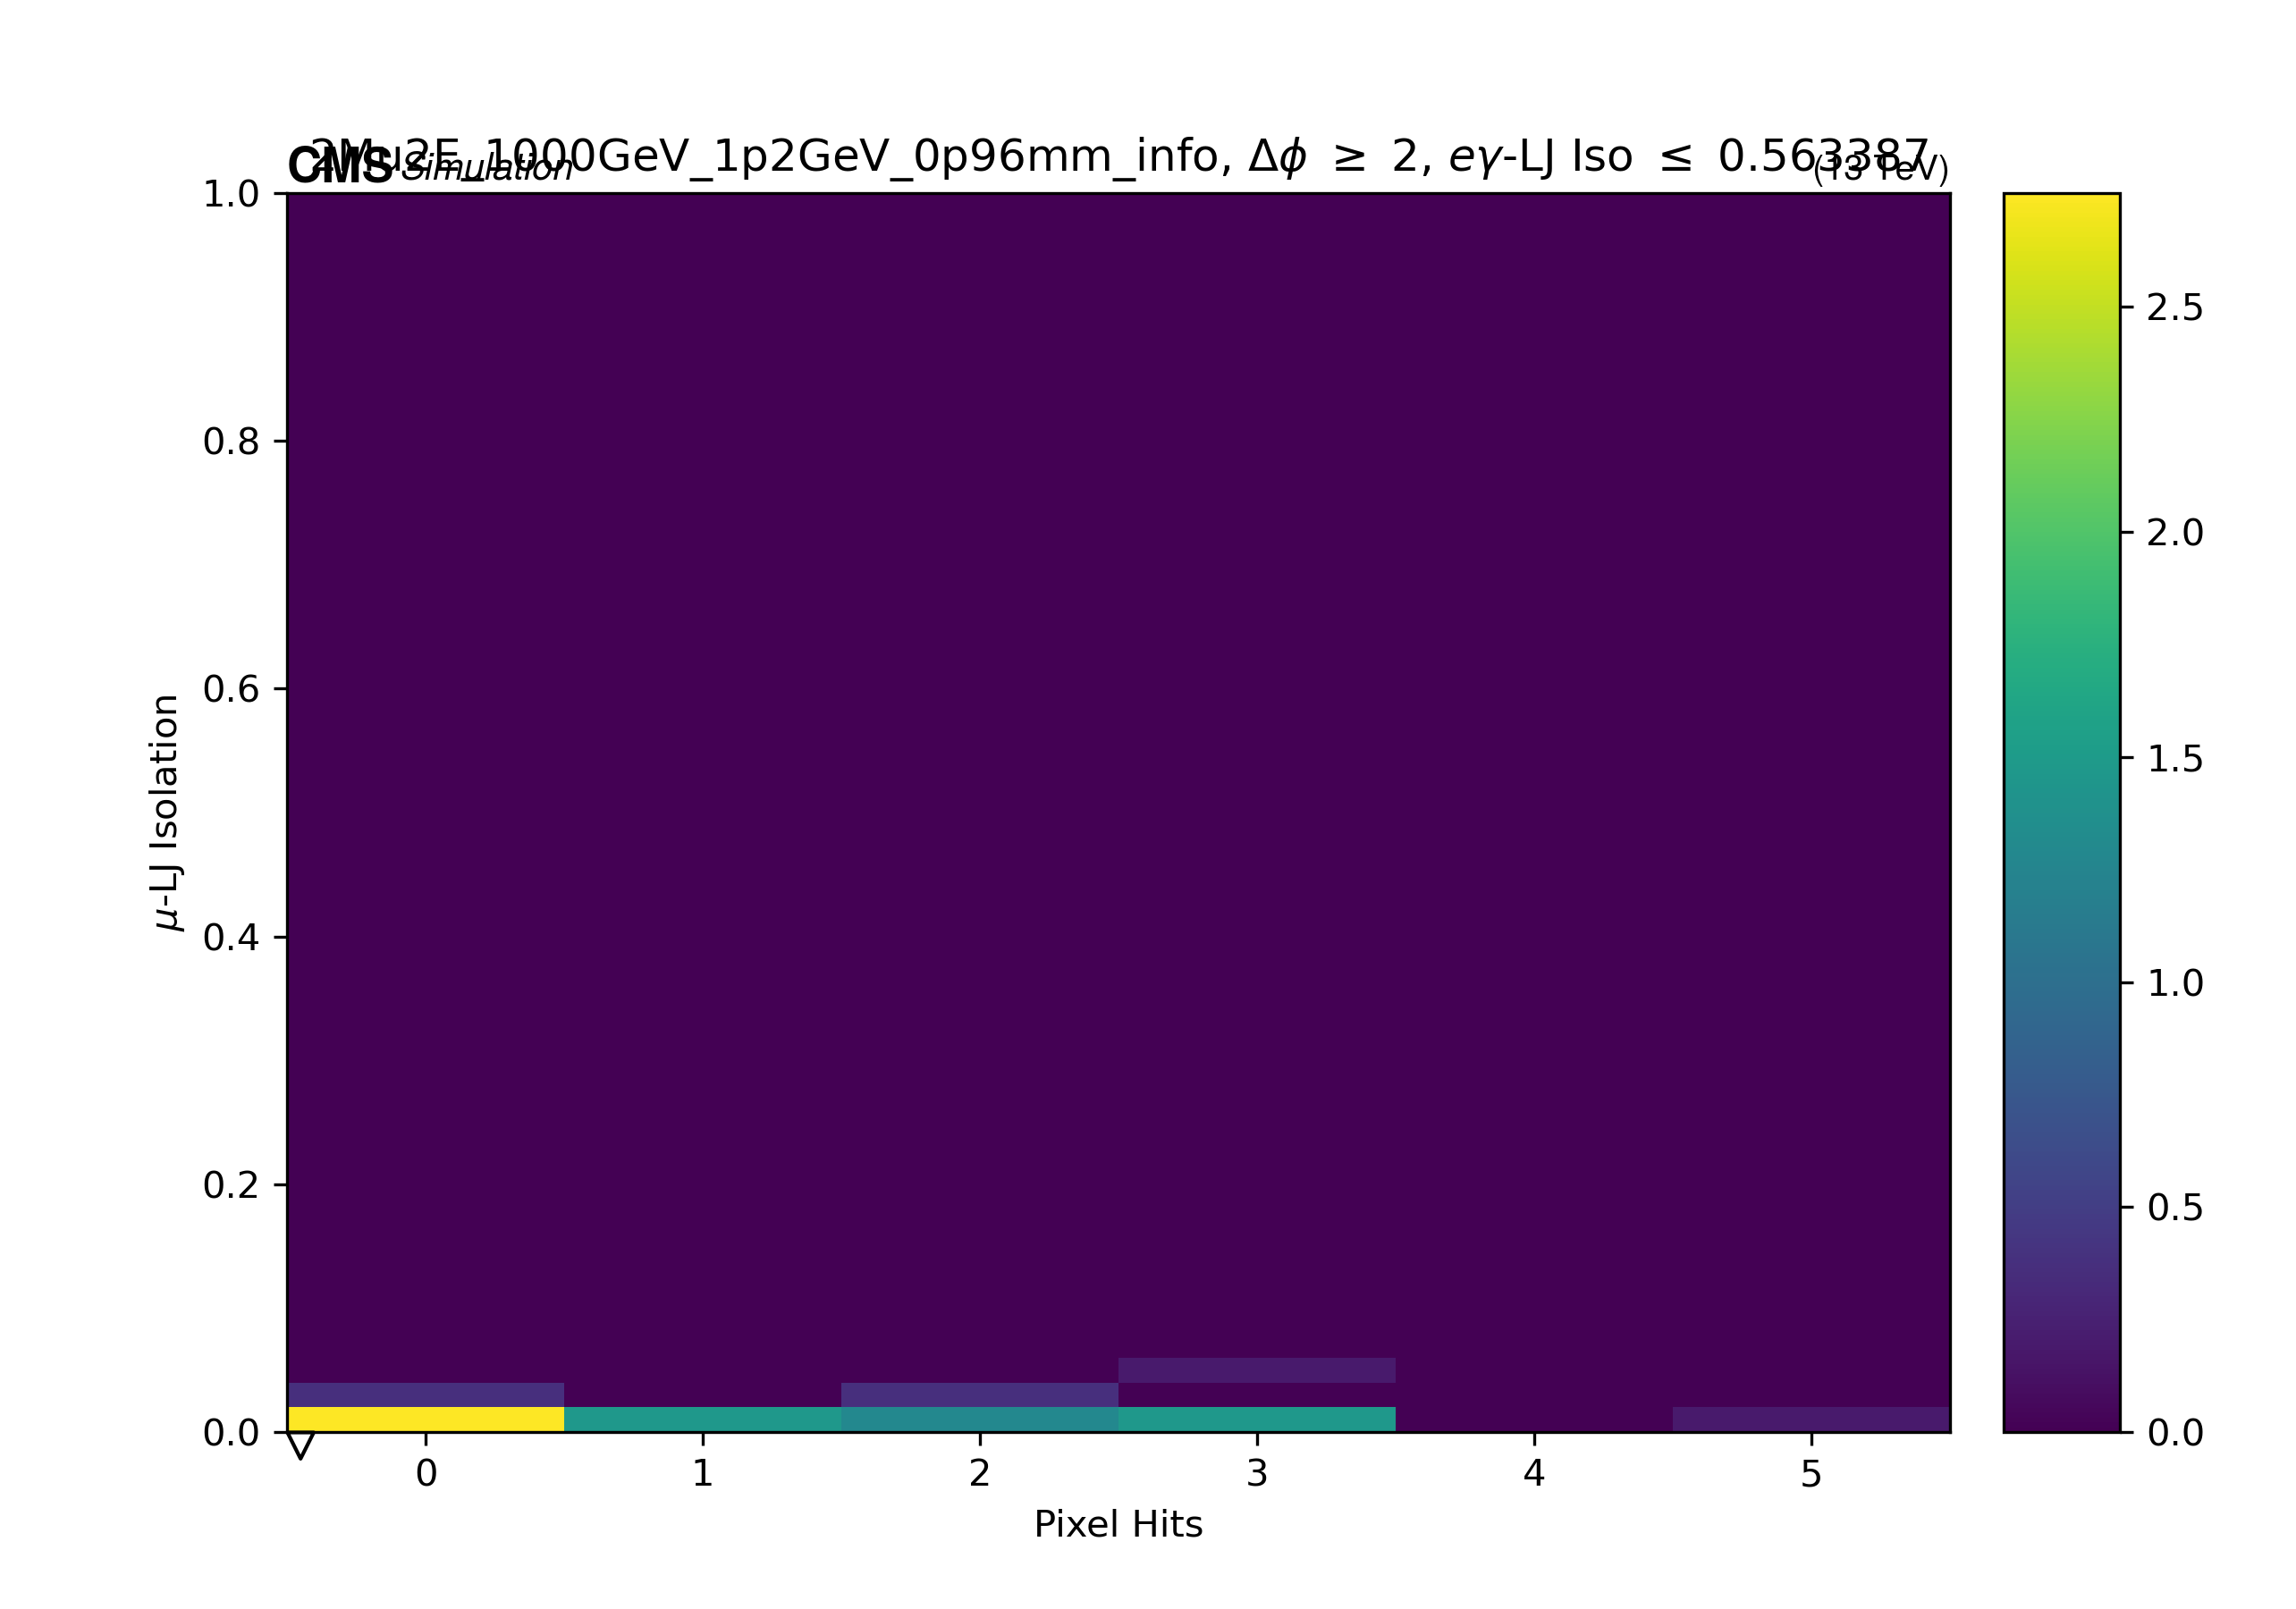
\includegraphics[width=\linewidth]{figures/2D_mJIso_vs_pixelHits_2Mu2E_1000GeV_1p2GeV_0p96mm_info.png}
		\end{column}
		\begin{column}{0.333\textwidth}
			\centering
			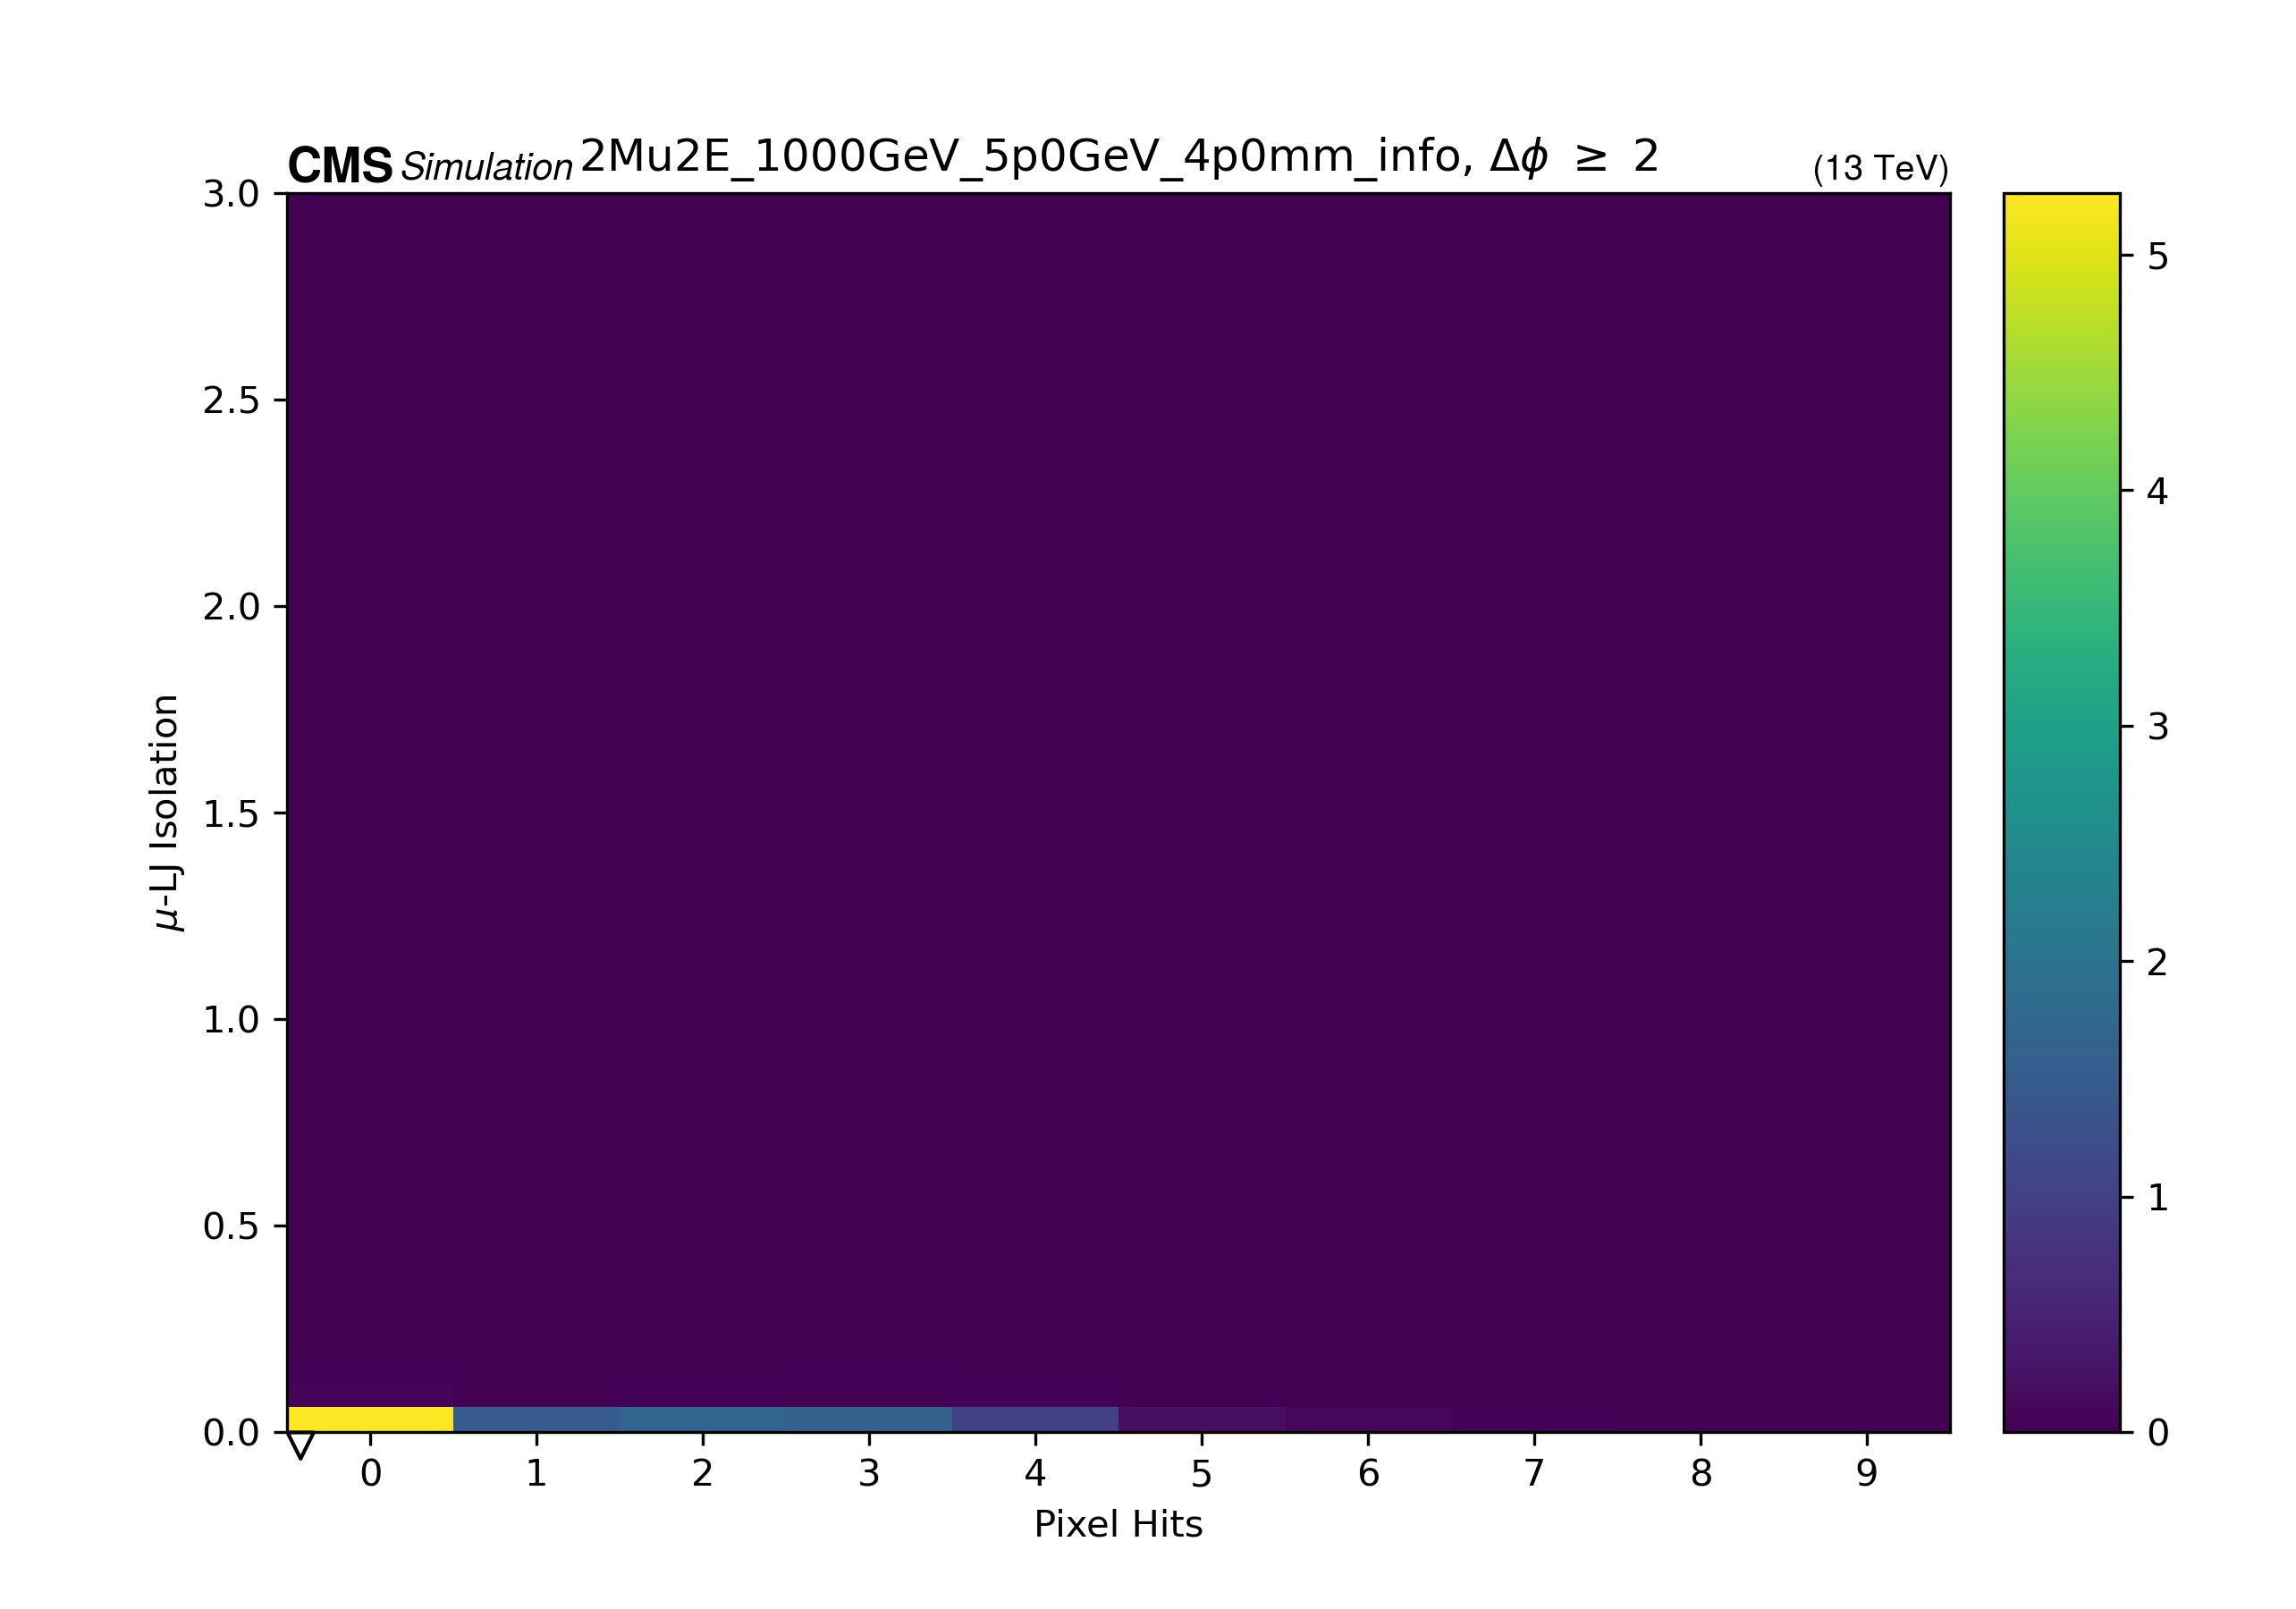
\includegraphics[width=\linewidth]{figures/2D_mJIso_vs_pixelHits_2Mu2E_1000GeV_5p0GeV_4p0mm_info.png}
		\end{column}
	\end{columns}
\end{frame}
% \section{Example Section} 
% \begin{frame}{single plot}
%             \centering
%             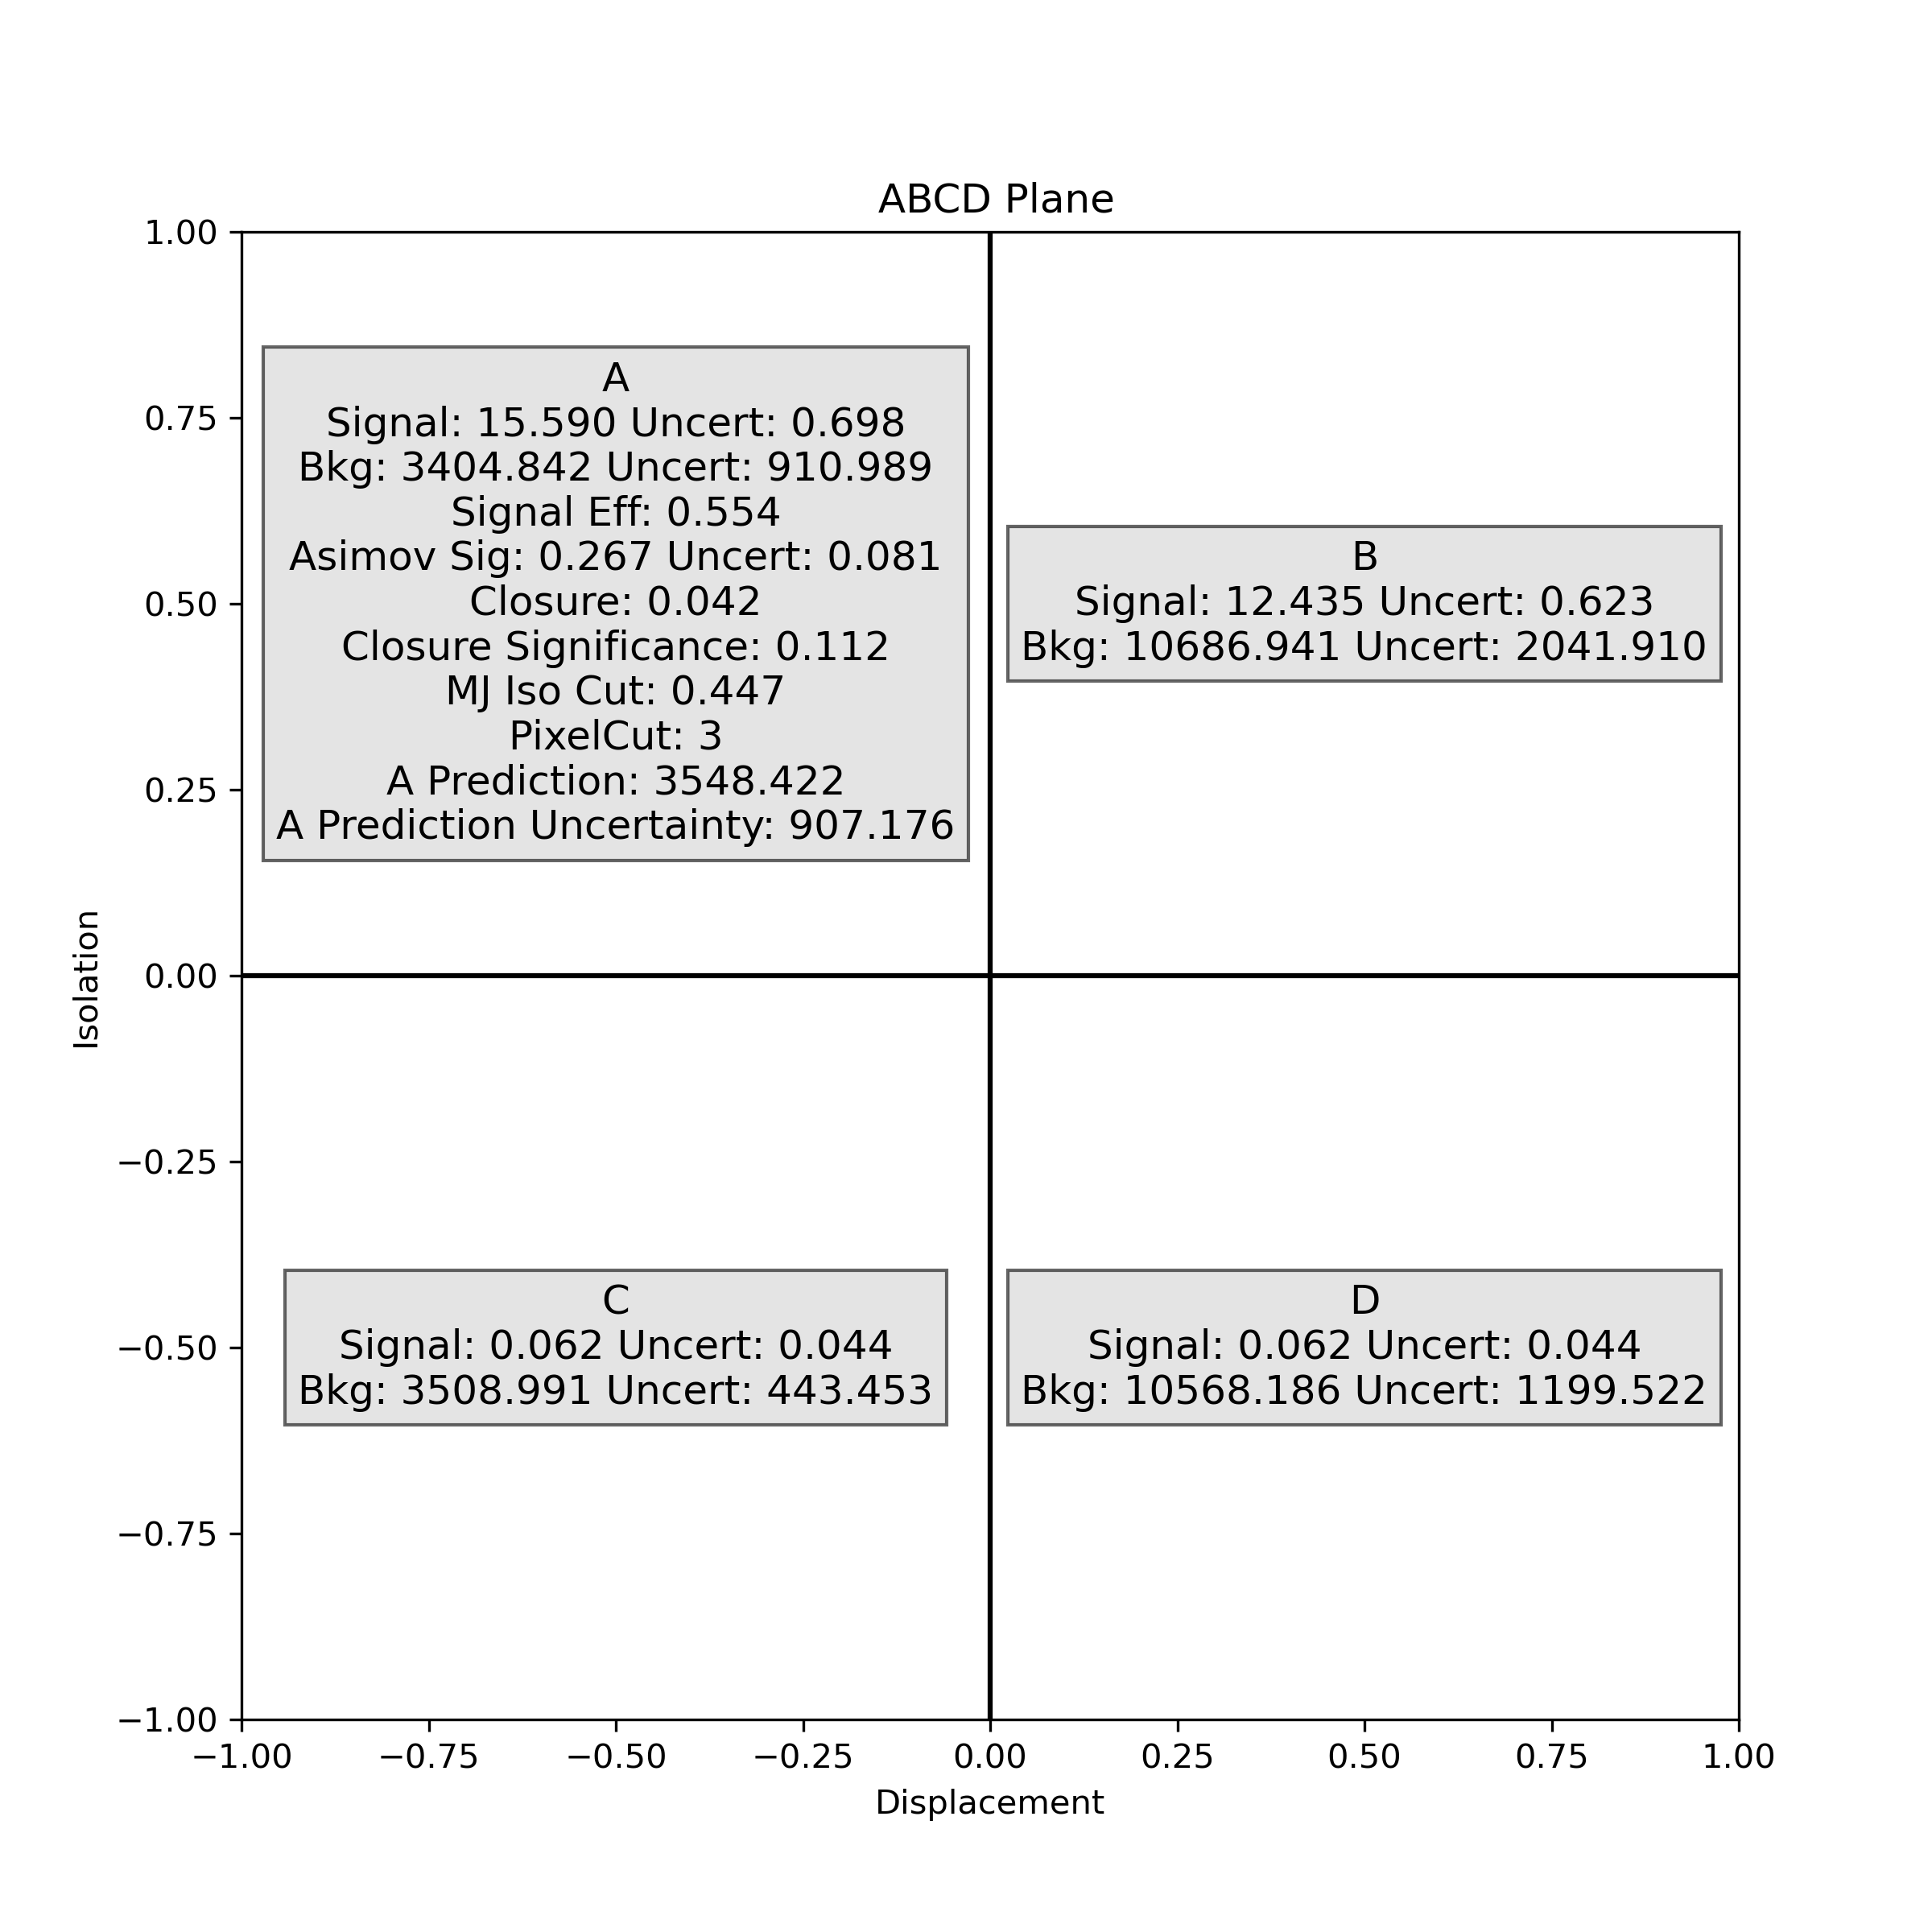
\includegraphics[width=0.5\linewidth]{figures/ABCDPlane_2Mu2E_200GeV_0p25GeV_0p1mm_info.png}
    
% \end{frame}

% \begin{frame}{multiple plots with text}
%     \begin{columns}
%         \begin{column}{0.5\textwidth}
%             \centering
%             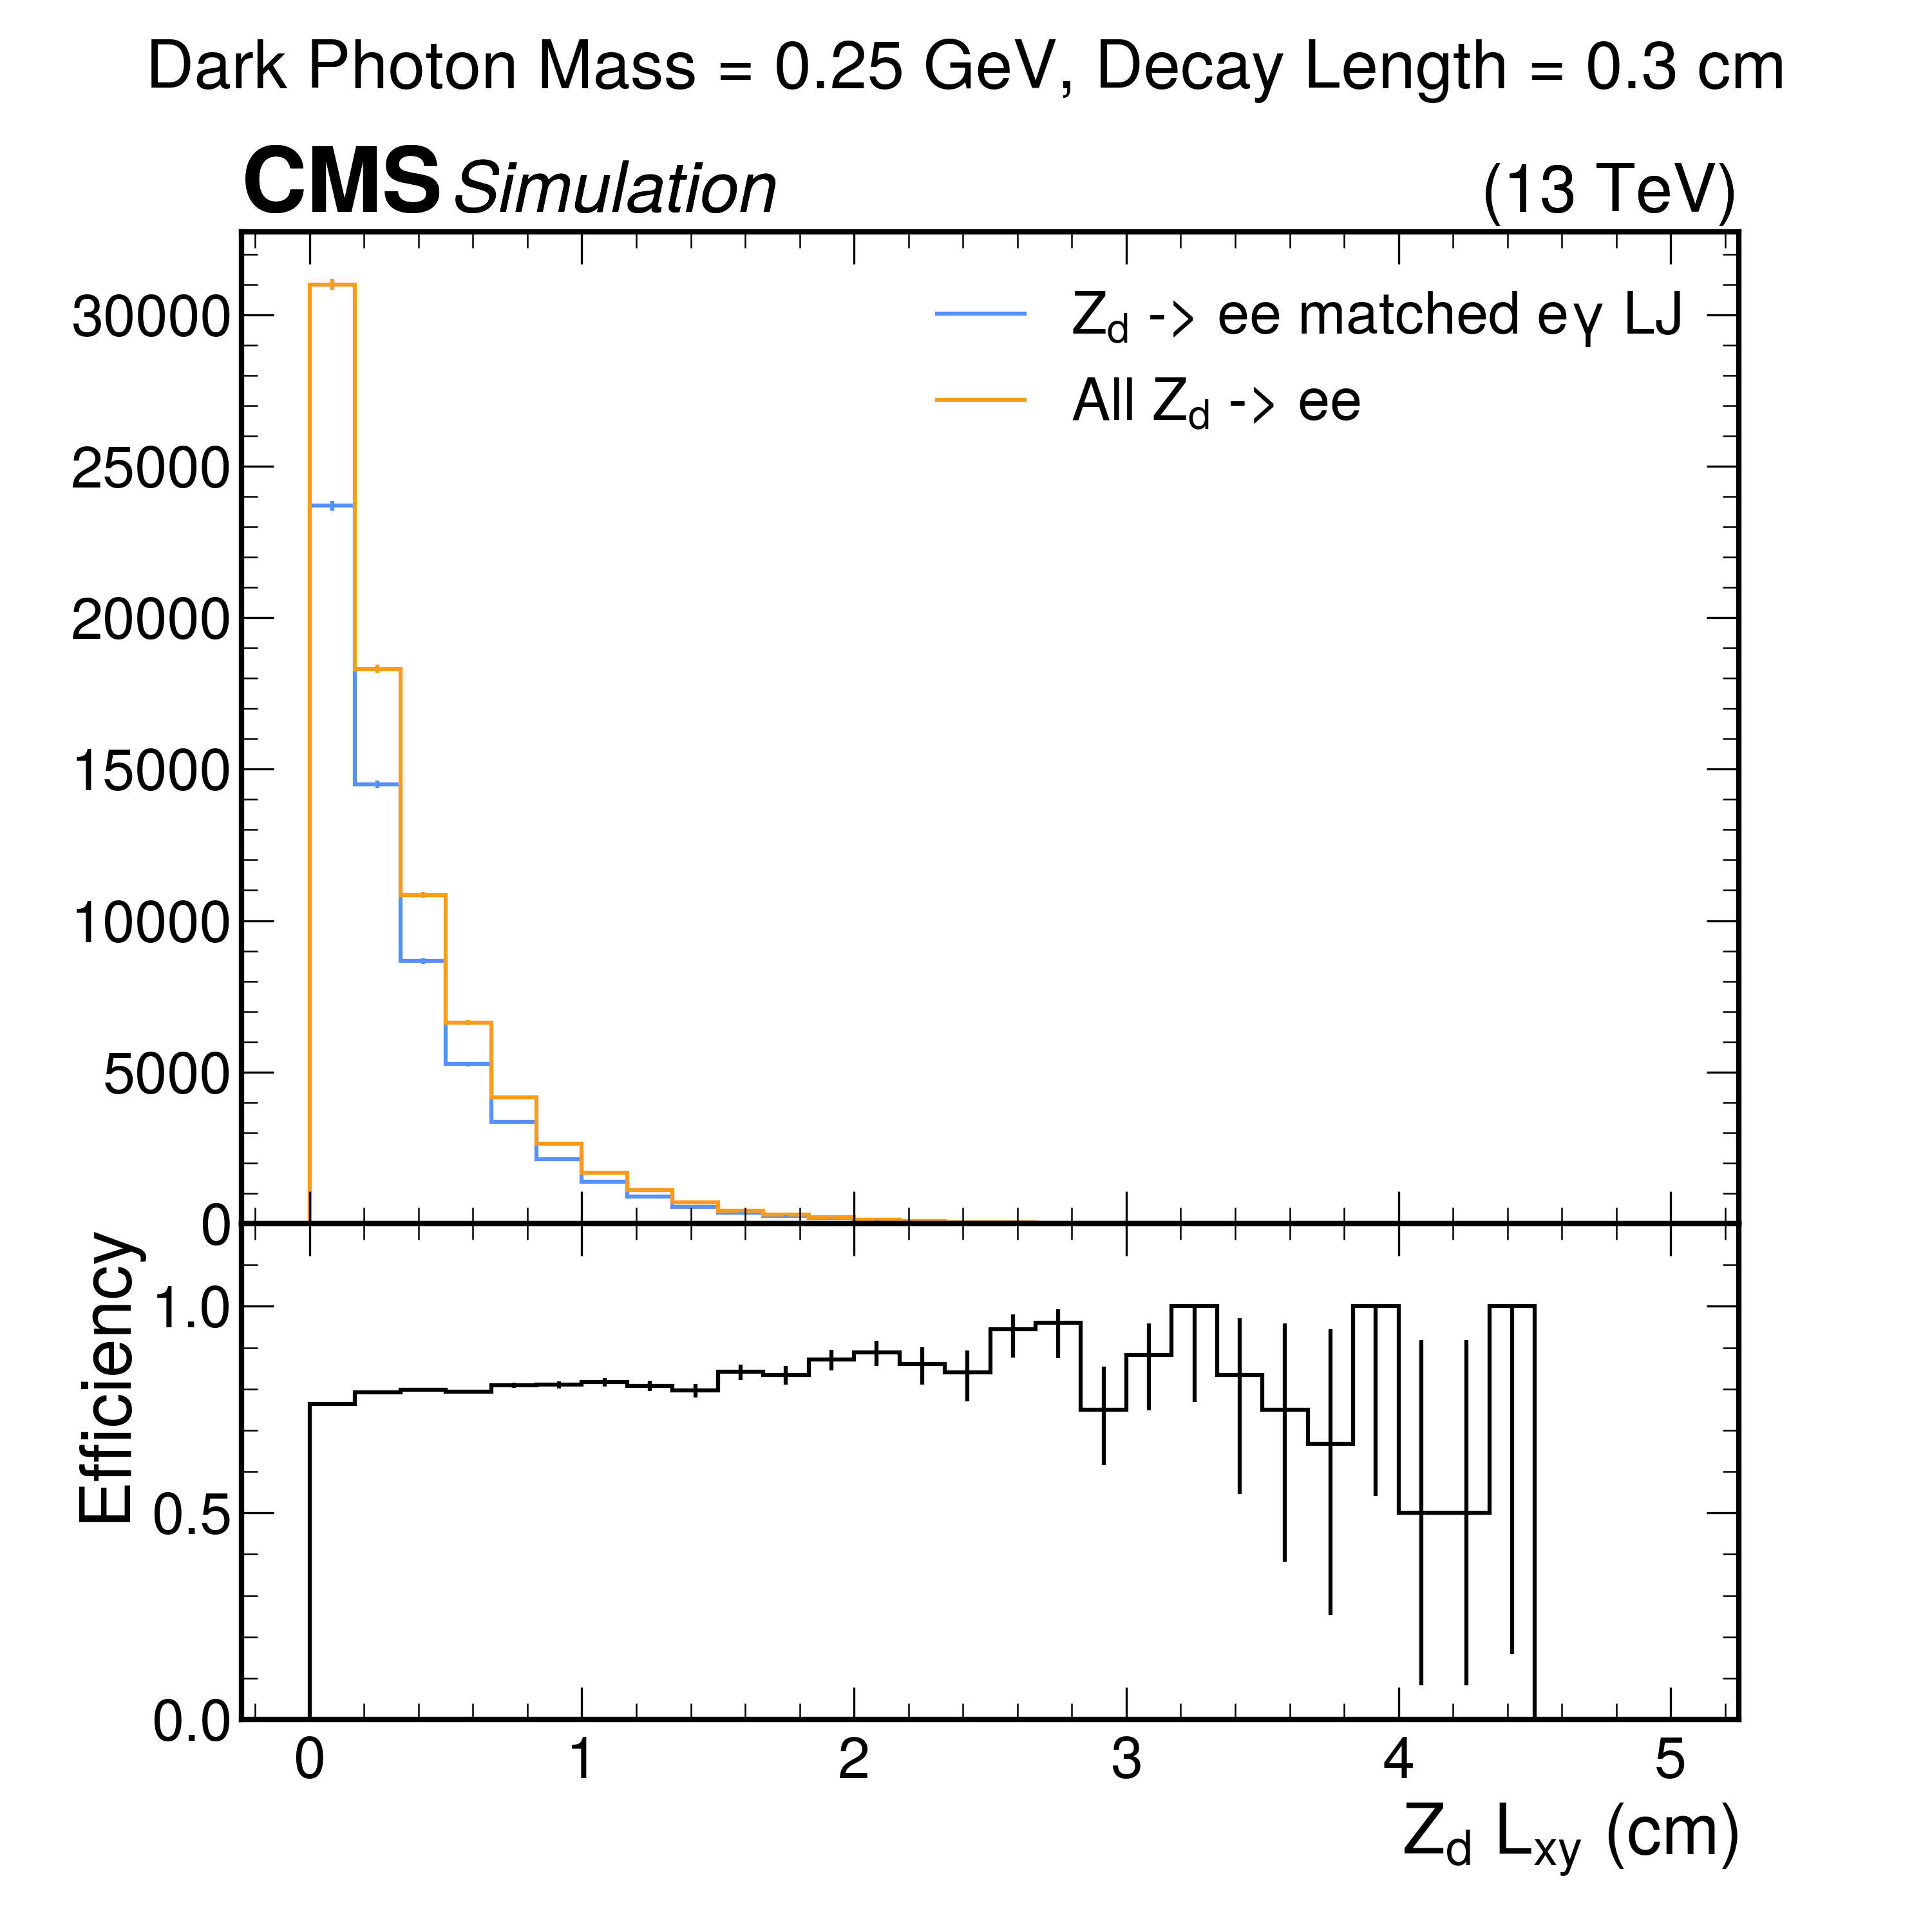
\includegraphics[width=0.65\linewidth]{figures/ratio_Lxy_2Mu2E_200GeV_0p25GeV_0p01mm_Loose-Loose.png}
%         \end{column}
%         \begin{column}{0.5\textwidth}
%             \centering 
%             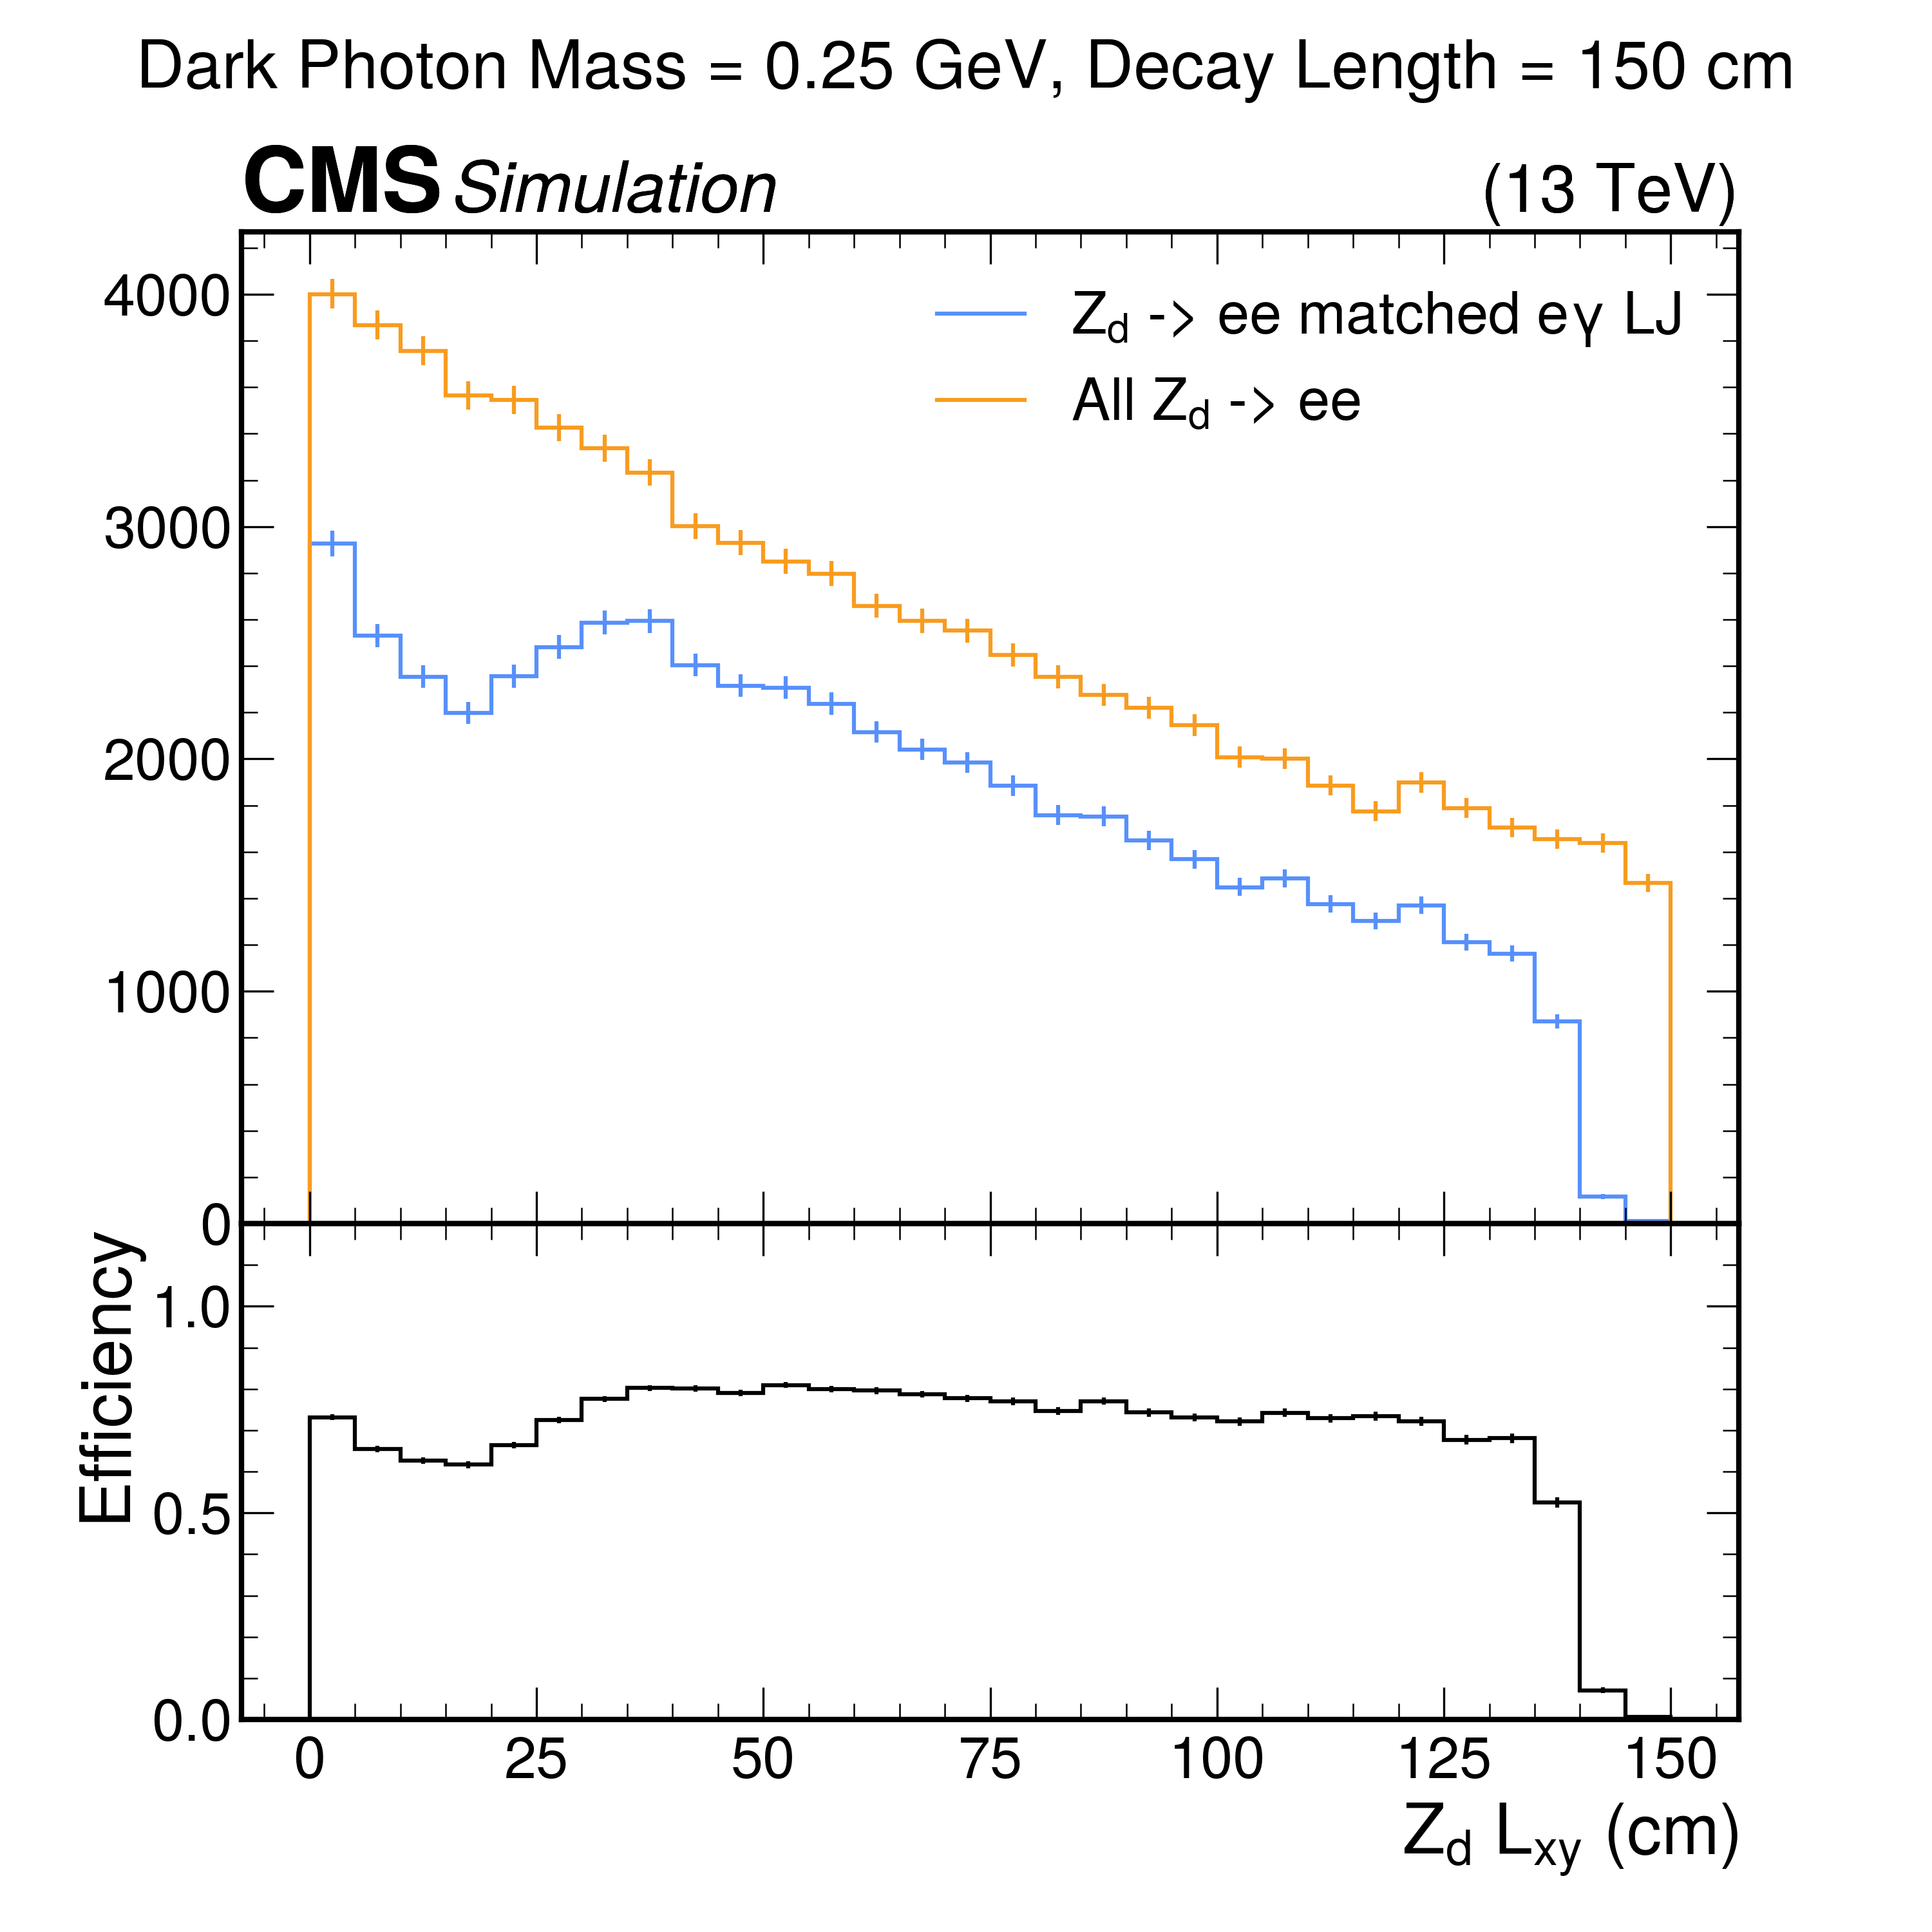
\includegraphics[width=0.65\linewidth]{figures/ratio_Lxy_2Mu2E_200GeV_0p25GeV_5p0mm_Loose-Loose.png}
%         \end{column}
%     \end{columns}
%     \textbf{Overall, not too many large changes in Reco Efficiency as a function of $L_{xy}$}
%     \begin{itemize}
%         \item At larger decay lengths ($L_{xy}$ > 0.3 cm), there seems to be a slight dip in reconstruction efficiency
%         \item The loss in efficiency points to an electron reconstruction issue
%         \begin{itemize}
%             \item The efficiency dips because our electron reconstruction suffers in the tracker, but we regain efficiency when electrons are reconstructed as photons in ECAL
%         \end{itemize}
%     \end{itemize}
% \end{frame}

\end{document}